\documentclass[blue,fullpaper]{ludusofficial}  % Theme: blue, red, green, purple, orange, cyan
                                              % Article type: fullpaper, letter, poster, survey, shortpaper, artpaper

%% Packages
\usepackage{amsmath}
\usepackage{tabularx}
\usepackage{graphicx} % Ecuaciones muy largas
\usepackage{amssymb}
\usepackage{placeins} %barreras moviles
\usepackage{cancel}
\usepackage{booktabs}

% Tipografia del informe: cuerpo de 10 pt, interlineado de 12 pt y titulos escalados por 10/8.5.
% Se aplica aqui porque la clase fija sus propios tamanos en \maketitle.
\makeatletter
\renewcommand{\normalsize}{\@setfontsize\normalsize{10}{12}}
\makeatother

% Fuentes matematicas: 8 pt; subindices de 6 pt y segundo nivel de 5 pt.
\DeclareMathSizes{10}{10}{8}{7}
\apptocmd{\maketitle}{\normalsize}{}{%
    \PackageError{informe}{No se pudo ajustar el cuerpo del informe}{}%
}
\patchcmd{\maketitle}{\fontsize{21}{35}}{\fontsize{24.7059}{41.1765}}{}{%
    \PackageError{informe}{No se pudo ajustar el titulo principal}{}%
}
\patchcmd{\maketitle}{\fontsize{11.5}{13.8}}{\fontsize{13.5294}{16.2353}}{}{%
    \PackageError{informe}{No se pudo ajustar el titulo del resumen}{}%
}
\patchcmd{\maketitle}{\fontsize{9}{10.35}}{\fontsize{10.5882}{12.1765}}{}{%
    \PackageError{informe}{No se pudo ajustar el texto del resumen}{}%
}
\titleformat{\section}
    {\fontsize{13.5294}{16.2353}\selectfont\sffamily\bfseries\color{themecolor}}
    {\thesection.}{0.5em}{}
\titleformat{\subsection}
    {\fontsize{12.3529}{14.8235}\selectfont\sffamily\bfseries\color{themecolor}}
    {\thesubsection.}{0.5em}{}
\titleformat{\subsubsection}
    {\fontsize{11.7647}{14.1176}\selectfont\sffamily\bfseries\color{darkgray}}
    {\thesubsubsection.}{0.5em}{}



%% Document metadata
\journalname{}
\journalsubtitle{}
\conferencename{}
\publicationyear{2026}
\institution{}  % This is now set by default in the class file
\journalurl{}  % This is now set by default in the class file
% \articletype{FULL PAPER}  % Set by document class option, or use \articletype{} to customize
%% DOI (optional - leave empty if not assigned yet)
% \articledoi{10.1234/ludus.2026.example}

%% Article information
\title{Proyecto Global Integrador: Control de Accionamiento de CA con Motor Sincrónico de Imanes Permanentes}
\shorttitle{Automática y Máquinas Eléctricas - Control de Accionamiento de CA con Motor Sincrónico de Imanes Permanentes}  % Short title for page headers
\shortauthor{Federico Barrios R. \& Lucia Muñiz}  % Short author names for page headers

\author{%
    \textbf{Federico Barrios R.}\textsuperscript{1}, \textbf{Lucia Muñiz}\textsuperscript{2}\\[0.2cm]
    \mdseries\small\textsuperscript{1}Facultad de Ingeniería, Universidad Nacional de Cuyo, Argentina\\
    \small\textsuperscript{2}Facultad de Ingeniería, Universidad Nacional de Cuyo, Argentina \\
    % \small Corresponding: john.smith@university.edu
}

\begin{document}


%% Abstract and keywords must be defined BEFORE \maketitle
\begin{abstract}
El presente informe corresponde al material obligatorio a entregar para acreditar el espacio curricular 311 "Automática y Máquinas Eléctricas". En el mismo, se desarrolla el estudio de un motor \textbf{Síncrono de Imanes Permanentes con control de accionamiento de C.A.} el cual es utilizado en una aplicación mecánica simplificada: el control de movimiento de un eje para la articulación de un brazo manipulador robótico elemental con \textbf{un solo grado de libertad} con un eje de rotación horizontal fijo a una base en el sistema de referencia inercial.

Las simulaciones son realizadas con el software propietario Simulink, de la empresa MathWorks, el actual estándar de la industria. En dichas simulaciones, se tienen en cuenta fenómenos de naturaleza mecánica, electromecánica, electromagnética y térmica para desarrollar un modelo físico y matemático que pueda representar fielmente los fenómenos que ocurren en la realidad. Además, se consideran casos en los cuales se utilizan coeficientes descriptivos promediados y casos en los cuales dichos variables tienen cierto grado de variación.

\end{abstract}


%% Maketitle creates full-width header with abstract and keywords, then starts two-column layout
\maketitle

\onecolumn
\tableofcontents
\clearpage
%%\twocolumn

\newpage

\section{Introducción}

Como se mencionó en el abstract, la aplicación de estudio es "el control de movimiento de un eje para la articulación de un brazo manipulador robótico elemental con \textbf{un solo grado de libertad} con un eje de rotación horizontal fijo a una base en el sistema de referencia inercial".

Con la intención de disminuir la complejidad, el sistema completo puede ser segmentado en un grupo de sistemas menores acoplados, los cuales se reconoce que son:

\begin{enumerate}
    \item \textbf{La carga.}\\Es el sistema del brazo robot, el cual responde unicamente a fenómenos mecánicos que pueden ser estudiado mediante herramientas de análisis de fuerzas (Ley de masa).
    \item \textbf{Tren de Transmisión.}\\Este sistema es el mediador entre el sistema de la carga y el sistema del motor (principal objeto de estudio). 
    \item \textbf{Máquina Eléctrica PMSM (motor).}\\Es el principal objeto de estudio y el más complejo. Puede ser descompuesto en 3 subsistemas:
    \begin{enumerate}
        \item \textbf{Subsistema Mecánico}: tomándose en cuenta al rotor referido a Estator estacionario, lo cual permite fijar al sistema inercial de referencia.
        \item \textbf{Subsistema Electromagnético}: El estudio de este subsistema se realizara con el uso de coordenadas electromagnéticas de rotor $dq0$ "fijas" al rotor, haciendo uso de \textit{la Transformada de Park}. Además, se considera valores de resistencias variables con la \textbf{temperatura}.
        \item \textbf{Subsistema Térmico}: modelo simplificado equivalente de primer orden que considera las pérdidas por calor.
    \end{enumerate}
    \item \textbf{Inversor Trifásico de Alimentación.}\\Inversor trifásico de 4 cuadrantes, consistente en un puente trifásico con llaves electrónicas semiconductoras, alimentado desde fuente de CC de tensión constante, conmutado con modulación de ancho de pulso, PWM 
    \item \textbf{Sensores de Retroalimentación.}\\El sistema global cuenta con los siguientes dispositivos físicos y sus canales de medición y acondicionamiento:
    \begin{enumerate}
        \item Un \textbf{(1)} sensor de \textbf{posición angular} montado en el \textbf{eje motor}.
        \item Tres \textbf{(3)} sensores de \textbf{corriente instantánea de fase}, montados en salida trifásica del inversor hacia bornes del estator.
        \item Un \textbf{(1)} sensor de \textbf{temperatura} en el bobinado del estator.
    \end{enumerate}
\end{enumerate}


% [Gráfico Ilustrativo (Tipo Mermaid)]
% Carga <-> Trasmición
% Trasmisión <-> Motor
% Motor <-> Alimentación
% Carga -> Sensores
% Motor -> Sensores
% Sensores -> Alimentación


La división del sistema global en estos subsistemas permite diferenciar y apreciar los fenómenos particulares de la aplicación, lo cual facilita el estudio al transformar el problema de un bloque complejo con varios fenómenos simultaneo a un sistema de varios bloques con fenómenos particulares acoplados entre ellos.

Con el afán de realizar un estudio completo, se analiza de manera concisa cada uno de los sistemas y sus modelos físicos, los cuales serán las bases para la modelación del sistema global y las diferentes solicitaciones pedidas.

% ---------------------------------------------------------------------------- %
\begin{figure}[htbp]
    \centering
    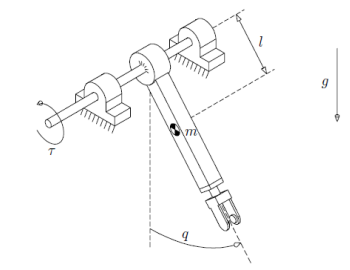
\includegraphics[width=0.5\linewidth]{attachments/image.png}
\end{figure}
\subsection{Carga}
El sistema de la carga responde a un modelo simplificado equivalente (No Lineal con parámetros variables) referido al eje de salida del tren de transmisión. La coordenada articular del eje de la articulación $q(t) \equiv \theta_l(t)$ referida a la vertical hacia abajo — lo que sería el punto de equilibrio estable. Las ecuaciones que describen este sistema son:

\begin{align}
    J_l \frac{d\omega_l(t)}{dt} & = T_q(t) - b_l \omega_l(t) - T_l(t) \label{eq:carga1} \\
    \frac{d\theta_l(t)}{dt}  & \equiv \omega_l(t)  \label{eq:Carga2}
\end{align}

donde, a su vez, los parámetros $T_l(t)$ y $\theta_l(t)$ cumplen también a las siguientes ecuaciones:
\begin{align*}
    T_{l}(t) & = gk_{l}\sin\big(\theta_{l}(t)\big) + T_{dl}(t)  \\
    \theta_{l}(t) & = \int_{0}^{t} \omega_{l}(\xi) \, d\xi + \theta_{l}(0)
\end{align*}

Los valores numéricos de las magnitudes físicas son como se menciona a continuación:

\begin{table}[htbp]
    \centering
    \caption{Coeficientes y datos del modelo base de la carga.}
    \label{tab:parametros_carga}
    % \small
    \begin{tabular}{lcc}
        \hline
        \textbf{Parámetro} & \textbf{Valor} & \textbf{Magnitud (Unidad)} \\
        \hline
        $b_l$ & $\approx 0.1 \pm 0.03$ & $\mathrm{Nm / (rad/s)}$ \\
        $m$ & $1.0$ & $\mathrm{kg}$ \\
        $l_{cm}$ & $0.25$ & $\mathrm{m}$ \\
        $J_{cm}$ & $0.0208$ & $\mathrm{kg \cdot m^{2}}$ \\
        $l_l$ & $0.50$ & $\mathrm{m}$ \\
        $m_l$ & $[0 \dots 1.5]$ & $\mathrm{kg}$ \\
        $J_l$ & $0.0833 + [0 \dots 0.375]$ & $\mathrm{kg \cdot m^{2}}$ \\
        $k_l$ & $0.25 + [0 \dots 0.75]$ & $\mathrm{kg \cdot m}$ \\
        $g$ & $9.80665$ & $\mathrm{m/s^2}$ \\
        \hline
    \end{tabular}
\end{table}

\begin{table}[htbp]
    \centering
    \caption{Especificaciones de operación de la carga.}
    \label{tab:parametros_carga}
    % \small
    \begin{tabular}{lcc}
        \hline
        \textbf{Parámetro} & \textbf{Valor} & \textbf{Magnitud (Unidad)} \\
        \hline
        $T_{ld}$ & $\approx 0 \pm 5.0$ & $\mathrm{Nm}$ \\
        \hline
    \end{tabular}
\end{table}


% ---------------------------------------------------------------------------- %
\subsection{Tren de Trasmisión}

El sistema del Tren de Trasmisión consta en una caja reductora reversible con sistema de engranajes planetarios, asumiendo acoplamiento rígido (sin elasticidad torsional y sin juego, holgura o “backlash”); momento de inercia equivalente y pérdidas de energía por fricción interna, reflejados al eje de entrada y considerados junto con el sistema de la PMSM (Máquina Eléctrica).

La ecuación que rige al sistema es:

\begin{align}
    \omega_{l}(t)  & = \frac{1}{r} \omega_{m}(t) \label{Transmision1}\\
    T_{q}(t)  & = r \cdot T_{d}(t)  \label{Transmision2}
\end{align}

Luego, los coeficientes del sistema y las especificaciones de operación del tren de transmisión tienen los siguientes valores:
\begin{table}[htbp]
    \centering
    \caption{Coeficientes y datos del modelo base del tren de transmisión.}
    \label{tab:parametros_carga}
    % \small
    \begin{tabular}{lcc}
        \hline
        \textbf{Parámetro} & \textbf{Valor} & \textbf{Magnitud (Unidad)} \\
        \hline
        $r$ & $120.0:1.0$ & $\mathrm{adim}$ \\
        \hline
    \end{tabular}
\end{table}

\begin{table}[htbp]
    \centering
    \caption{Especificaciones de operación del tren de trasmisión.}
    \label{tab:parametros_carga}
    % \small
    \begin{tabular}{lcc}
        \hline
        \textbf{Parámetro} & \textbf{Valor} & \textbf{Magnitud (Unidad)} \\
        \hline
        $n_{l \; \mathrm{nom}}$ & $60$ & $\mathrm{rpm}$ \\
        $T_{q \; \mathrm{nom}}$ & $17.0$ & $\mathrm{Nm}$ \\
        $T_{q \; \mathrm{max}}$ & $45.0$ & $\mathrm{Nm}$ \\
        \hline
    \end{tabular}
\end{table}


Estos parámetros no deberán ser superados durante el periodo de trabajo.

% ---------------------------------------------------------------------------- %
\subsection{PMSM (Máquina Eléctrica)}
La Máquina Síncrona de Imanes Permanentes (PMSM) cuenta con estátor simétrico y equilibrado, con bornes de fase $abc$ conectadas externamente en estrella (Y), con centro O flotante (no accesible) y bornes de línea $ABC$ accesibles desde el inversor electrónico trifásico.

Las especificaciones de operación de este sistema son:

\begin{table}[htbp]
    \centering
    \caption{Especificaciones de operación del motor en bornes de fases $abcs$ de estator (valores límite, no sobrepasar).}
    \label{tab:parametros_carga}
  %   \small
    \begin{tabular}{lcc}
        \hline
        \textbf{Parámetro} & \textbf{Valor} & \textbf{Magnitud (Unidad)} \\
        \hline
        $n_{m \; \mathrm{nom}}$ & $6600$ & $\mathrm{rpm}$ \\
        $V_{sl \; \mathrm{nom}}$ & $30.0$ & $\mathrm{V_{ca \; RMS}}$ \\
        $I_{s \; \mathrm{nom}}$ & $0.4$ & $\mathrm{A_{ca \; RMS}}$ \\
        $I_{s \; \mathrm{max}}$ & $2.0$ & $\mathrm{A_{ca \; RMS}}$ \\
        $T_{s \; \mathrm{max}}^{\circ}$ & $115.0$ & $\mathrm{{}^{\circ}C}$ \\
        $T_{\mathrm{amb}}$ & $[-15 ... 40]$ & $\mathrm{{}^{\circ}C}$ \\
        \hline
    \end{tabular}
\end{table}

Recordando, este sistema se desacopla en 3 subsistemas, a decir:




\subsubsection{Subsistema Mecánico}
Las ecuaciones que de este sistema son similares a las del sistema de la carga:

\begin{align}
    J_m \frac{d\omega_m(t)}{dt} &= T_m(t) - b_m \omega_m(t) - T_d(t) \label{SubMec1}\\
    \frac{d\theta_m(t)}{dt} &\equiv \omega_m(t)  \label{SubMec2}
\end{align}

donde $\theta_m$ también puede calcularse como:
\[
\theta_{m}(t) = \int_{0}^{t} \omega_{m}(\xi) \, d\xi + \theta_{m}(0) 
\]

Los valores de los coeficientes de este subsistema son:
\begin{table}[htbp]
    \centering
    \caption{Coeficientes y datos del subsistema mecánico.}
    \label{tab:parametros_carga}
%    \small
    \begin{tabular}{lcc}
        \hline
        \textbf{Parámetro} & \textbf{Valor} & \textbf{Magnitud (Unidad)} \\
        \hline
        $J_m$ & $\approx 14.0 \times 10^{-6}$ & $\mathrm{\mathrm{kg \; m}}$ \\
        $b_m$ & $\approx 15.0 \times 10^{-6}$ & $\mathrm{\mathrm{\frac{Nm}{rad/s}}}$ \\
        \hline
    \end{tabular}
\end{table}

\subsubsection{Subsistema electromagnético}
El subsistema electromagnético responde a un modelo idealizado equivalente en coordenadas de roto $dq0^r$ "fijas" al rotor. Para el estudio de este subsistema se utiliza la Transformación de Park en el circuito del estator estacionario. Teniendo en cuenta que las siguientes ecuaciones trabajan en el espacio de Park, el subsistema electromagnético puede ser modelado con las siguientes expresiones matemáticas:

\begin{itemize}
    \item Relación entre el espacio inercial y el espacio de Park
    \begin{align}
    \frac{d\theta_{r}(t)}{dt}  & \equiv \omega_{r}(t) \label{SubElec1}\\
    \theta_{r}(t)  & \equiv P_{p} \theta_{m}(t)  \label{SubElec2}
    \end{align}
    \item Balance de tensiones eléctricas equivalentes de estator y cálculo del torque electromagnético producido por el motor
    \begin{align}
        T_{m}(t) &  = \frac{3}{2}P_{p} \lambda_{m}^{'r} i_{qs}^{r}(t) + \frac{3}{2} P_{p} \Big( L_{d} - L_{q} \Big) i_{qs}^{r}(t) i_{ds}^{r}(t) \label{SubElec3} \\
        v_{qs}^{r}(t) & = R_{s} \Big( T_{s}^{\circ} (t) \Big) i_{qs}^{r}(t) + L_{q} \frac{di_{qs}^{r}(t)}{dt}  + \Big[ \lambda_{m}^{'r} + L_{d} i_{ds}^{r}(t) \Big] \omega_{r}(t)\label{SubElec4} \\
        v_{ds}^{r}(t) & = R_{s} \Big( T_{s}^{\circ} (t) \Big) i_{ds}^{r}(t) + L_{d} \frac{di_{ds}^{r}(t)}{dt} - L_{q}i_{qs}^{r}(t) \omega_{r}(t)   \label{SubElec5}\\
        v_{0s}^{r}(t) & = R_{s} \Big( T_{s}^{\circ} (t) \Big) i_{0s}^{r}(t) + L_{ls} \frac{di_{0s}^{r}(t)}{dt} \label{SubElec6}
    \end{align}
\end{itemize}

Los valores de los coeficientes de este subsistema son:

\begin{table}[htbp]
    \centering
    \caption{Coeficientes y datos del subsistema electromagnético.}
    \label{tab:parametros_carga}
 %   \small
    \begin{tabular}{lcc}
        \hline
        \textbf{Parámetro} & \textbf{Valor} & \textbf{Magnitud (Unidad)} \\
        \hline
        $P_p$ & $3$ & Pares de Polos \\
        $\lambda_{m}^{'r}$ & $0.016$ & $\mathrm{\frac{V}{rad/s}}$ \\
        $L_q$ & $5.8$ & $\mathrm{mH}$ \\
        $L_s$ & $6.6$ & $\mathrm{mH}$ \\
        $L_{ls}$ & $0.8$ & $\mathrm{mH}$ \\
        \hline
    \end{tabular}
\end{table}

\subsubsection{Subsistema Térmico}
El subsistema térmico consta de un modelo simplificado equivalente de primer orden, considerando sólo pérdidas eléctricas resistivas por efecto Joule (calor) en bobinado de estator, despreciando pérdidas magnéticas en el núcleo; transferencia de calor al ambiente solo por conducción y convección natural y sin ventilación forzada.

Las ecuaciones que representan la variación del valor de las resistencias de bobinado y las pérdidas por calor se expresan como:

\begin{align}
    R_{s}(T_{s}^{\circ}(t)) & = R_{sREF} \Big(1 + \alpha_{Cu} (T_{s}^{\circ}(t) - T_{sREF}^{\circ}) \Big) \label{SubTerm1}\\
    P_{s \; \text{perdida}}(t)  & = R_{s}(T_{s}^{\circ}(t)) \Big( i_{as}^{2}(t) + i_{bs}^{2}(t) + i_{cs}^{2}(t) \Big) \\
     & = R_{s}(T_{s}^{\circ}(t)) \frac{3}{2} \Big( i_{qs}^{r\;2}(t) + i_{ds}^{r\;2}(t) + 2i_{0s}^{r\;2}(t) \Big) \\
     & = C_{ts} \frac{dT_{s}^{\circ}(t)}{dt} +  \frac{T_{s}^{\circ}(t) - T_{amb}^{\circ}(t)}{R_{ts-amb}}
\end{align}

Como se puede ver, las ecuaciones (\ref{SubTerm2}) y (\ref{SubTerm3}) son las formas de calcular las pérdidas de potencia por calor debido a efecto Jouls — ya sea teniendo en cuenta las corrientes de bornes o las corrientes virtuales del espacio de Park — y también son equivalentes a la perdida de potencia deducida por el balance térmico de la PMSM. Más adelante se hablará de la Transformada de Park, pero resulta coherente que el cambio variables de tensión de bornes (tensiones abc) y tensiones virtuales (tensiones $dq0$) expresen la misma potencia, puesto que ambos representan el mismo fenómeno (no se crea ni destruye energía).

Los valores de los coeficiente son:

\begin{table}[htbp]
    \centering
    \caption{Coeficientes y datos del subsistema térmico.}
    \label{tab:parametros_carga}
  %  \small
    \begin{tabular}{lcc}
        \hline
        \textbf{Parámetro} & \textbf{Valor} & \textbf{Magnitud (Unidad)} \\
        \hline
        $R_s$ & $\approx 1.02$ & $\Omega$ \\
        $\alpha_{Cu}$ & $3.9 \times 10^{-3}$ & $\mathrm{\frac{1}{{}^\circ C}}$ \\
        $C_{ts}$ & $0.818$ & $\mathrm{\frac{W}{{}^\circ C/s}}$ \\
        $R_{ts-amb}$ & $146.7$ & $\mathrm{\frac{{}^\circ C}{W}}$ \\
        \hline
    \end{tabular}
\end{table}

Cabe la pena destacar que la resistencia de bobinados $R_s \approx 1.02 \Omega$ es el valor de referencia de la resistencia a temperatura de $20^{\circ}C$, es decir: $R_s \approx 1.02 \Omega = R_{s \; REF} \Big( @ \; T_{s \; REF}=25^\circ C \Big)$

% ---------------------------------------------------------------------------- %
\subsection{Inversor Trifásico de Alimentación}
El sistema del Inversor trifásico de 4 cuadrantes (regenerativo), consiste en un puente trifásico con llaves electrónicas semiconductoras  alimentado desde fuente de CC de tensión constante, conmutado con modulación de ancho de pulso, PWM.

Se asume inicialmente el Modulador de tensión trifásico (vectorial) sin límite de tensión, con respuesta ideal $G(s) \equiv 1$ (filtro “pasatodo”, ganancia unitaria y ancho de banda “infinito”). En un estudio posterior, esta hipótesis será modificada.

Las ecuaciones que modelan este sistema son:

\begin{align}
    \frac{d\theta_{ev}(t)}{dt}  & \equiv 2\pi f_{e}(t) \equiv \omega_{e}(t) \\
    \delta(t)  & \equiv \theta_{ev}(t) - \theta_{r}(t) \\ 
    v_{as}(t)  & \cong \sqrt{ 2 } \frac{V_{sl}(t)}{\sqrt{ 3 }} \cos \Big( \theta_{ev}(t) \Big)  \\
    v_{bs}(t) &  \cong \sqrt{ 2 } \frac{V_{sl}(t)}{\sqrt{ 3 }} \cos \Big( \theta_{ev}(t) - \frac{2\pi}{3} \Big) \\
    v_{cs}(t) &  \cong \sqrt{ 2 } \frac{V_{sl}(t)}{\sqrt{ 3 }} \cos \Big( \theta_{ev}(t) + \frac{2\pi}{3}  \Big)
\end{align}

De aquí, se puede apreciar como las tensiones que alimentan el motor son controladas única y exclusivamente con los parámetros $V_{sl}(t)$ y $\omega_e(t)\equiv 2\pi \; f_e(t)$, los cuales son los parámetros manipulados por el operador (nosotros).

Además, aparece $\delta(t)$ — ángulo de desfasaje electromagnético de rotor — el cual representa el desfasaje instantáneo relativo entre la coordenada eléctrica sincrónica $\theta_{ev}$ (tensión de fase $a$ del estator) y la coordenada eléctrica fija a rotor $\theta_r$ (respecto al espacio $dq0^r$). Esta última depende del torque electromagnético.

\begin{table}[htbp]
    \centering
    \caption{Especificaciones de operación del sistema de Alimentación.}
    \label{tab:parametros_carga}
   % \small
    \begin{tabular}{lcc}
        \hline
        \textbf{Parámetro} & \textbf{Valor} & \textbf{Magnitud (Unidad)} \\
        \hline
        $V_{sl}$ & $[0.0 ... 48]$ & $\mathrm{V_{ca \; RMS}}$ \\
        $f_e$ & $[-330 ... 0 ... +330]$ & $\mathrm{Hz}$ \\
        \hline
    \end{tabular}
\end{table}

Se debe tener en cuenta que el signo de $f_e$ ($\pm$) determina la secuencia de fases positiva (abc) ó negativa (acb) y por consiguiente, el sentido de giro del campo magnético rodante y del rotor.

% ---------------------------------------------------------------------------- %
\subsection{Sensores de Retroalimentación}
Para la medición y acondicionamiento de las señales de realimentación indispensables para el lazo cerrado, el sistema incorpora los siguientes dispositivos físicos:

\begin{itemize}
    \item \textbf{Un (1) sensor de posición angular:} Consiste en un codificador incremental (\textit{encoder}) montado en el eje motor. Teniendo un proceso de \textit{homing} y decodificación ideal, registra la posición angular absoluta ``rectificada'' $\theta_m(t)$. Esta variable se vincula a la coordenada articular de la carga mediante la relación mecánica $\theta_l(t) = \frac{1}{r} \theta_m(t)$, estableciéndose un ajuste de origen tal que $\theta_m \equiv 0$ cuando $\theta_l \equiv 0$.
    \item \textbf{Tres (3) sensores de corriente instantánea:} Consisten en amperímetros montados en la salida trifásica del inversor electrónico hacia los bornes del estator. Miden las corrientes reales de fase $i_a(t)$, $i_b(t)$ e $i_c(t)$, las cuales permiten la reconstrucción de las corrientes virtuales del espacio de Park ($i_{qs}^r$, $i_{ds}^r$, $i_{0s}^r$) mediante la Transformada de Park.
    \item \textbf{Un (1) sensor de temperatura:} Consiste en un sensor instalado en el bobinado del estator. Registra la variable térmica $T_s^\circ(t)$ empleada para el monitoreo de calentamiento, la protección ante sobretemperaturas y el cálculo constante de la variación de la resistencia del estator $R_s(T_s^\circ(t))$.
\end{itemize}

%\begin{quote}
 %   \textbf{Nota sobre el modelo de respuesta:} Inicialmente, para el análisis dinámico a lazo abierto y el diseño de la ley de control por retroalimentación, se asume un comportamiento ideal para todos los transductores, caracterizado por una función de transferencia unitaria $G(s) \equiv 1$ (ganancia unitaria, filtro ``pasa todo'' y ancho de banda infinito).
%\end{quote}

\subsection{Espacio de Park}

En la década de 1920, R.H. Park introdujo una nueva forma de analizar máquinas eléctricas: formuló un cambio de variables que reemplaza, de forma efectiva, las variables asociadas a los devanados del estator de una máquina síncrona por variables asociadas a devanados ficticios que rotan a la velocidad angular eléctrica del rotor.

La transformada de Park tiene la propiedad única de eliminar las inductancias dependientes de la posición del rotor en las ecuaciones de tensión de las máquinas síncronas, las cuales surgen debido a circuitos eléctricos con movimiento relativo entre sí y a circuitos con diferentes valores de reluctancia magnética.

Pese a que la transformación de variables se refiere a un marco de referencia arbitrario y no requiere una connotación física, suele ser conveniente visualizar las ecuaciones de transformación como relaciones trigonométricas entre variables. Específicamente, resulta útil interpretar a $f_{qs}$ y $f_{ds}$ como variables dirigidas en trayectorias ortogonales entre sí y que rotan a una velocidad angular $\omega$, mientras que $f_{as}$, $f_{bs}$ y $f_{cs}$ son consideradas variables dirigidas en trayectorias estacionarias desplazadas $120^{\circ}$ entre sí.

\newpage

\begin{figure}
    \centering
    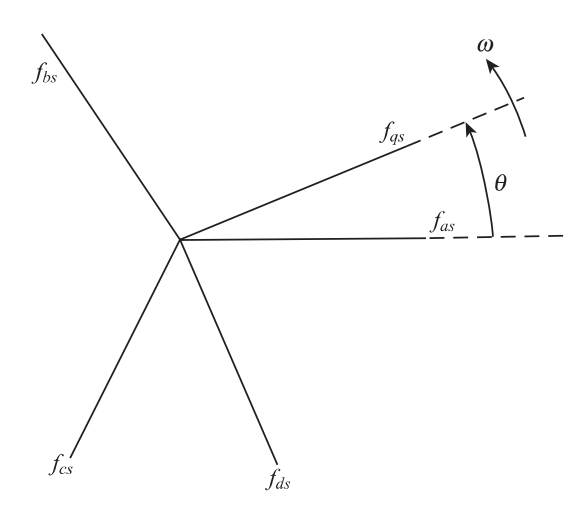
\includegraphics[width=0.5\linewidth]{attachments/TransformadaDePark.png}
    \caption{Interpretación Gráfica}
\end{figure}

Dependiendo del valor de la velocidad angular eléctrica $\omega$ elegida para realizar la transformación de variables, se suele utilizar la siguiente convención para referirse a las diferentes trasnformadas:

\begin{table}[htpb]
    \centering
    \renewcommand{\arraystretch}{1.5} % Da respiro vertical a las filas
    \begin{tabular}{@{}llcc@{}}
        \toprule
        & & \multicolumn{2}{c}{Notation} \\ \cmidrule(l){3-4}
        \begin{tabular}[c]{@{}l@{}}Reference-\\ Frame Speed\end{tabular} & 
        \multicolumn{1}{c}{Interpretation} & 
        Variables & 
        Transformation \\
        \midrule
        
        $\omega$ (unspecified) & 
        \begin{tabular}[c]{@{}c@{}}Stationary circuit variables referred to an \\ arbitrary reference frame\end{tabular} & 
        \begin{tabular}[c]{@{}c@{}}$\mathbf{f}_{dq0s}$ or $f_{ds}, f_{qs},$\\ $f_{0s}$\end{tabular} & 
        $\mathbf{K}_s$ \\
        
        $0$ & 
        \begin{tabular}[c]{@{}c@{}}Stationary circuit variables referred to a \\ stationary reference frame\end{tabular} & 
        \begin{tabular}[c]{@{}c@{}}$\mathbf{f}^s_{dq0s}$ or\\ $f^s_{ds}, f^s_{qs}, f_{0s}$\end{tabular} & 
        $\mathbf{K}^s_s$ \\
        
        $\omega_r$ & 
        \begin{tabular}[c]{@{}c@{}}Stationary circuit variables referred to a \\ reference frame fixed in the rotor\end{tabular} & 
        \begin{tabular}[c]{@{}c@{}}$\mathbf{f}^r_{dq0s}$ or\\ $f^r_{ds}, f^r_{qs}, f_{0s}$\end{tabular} & 
        $\mathbf{K}^r_s$ \\
        
        $\omega_e$ & 
        \begin{tabular}[c]{@{}c@{}}Stationary circuit variables referred to a \\ synchronously rotating reference frame\end{tabular} & 
        \begin{tabular}[c]{@{}c@{}}$\mathbf{f}^e_{dq0s}$ or \\ $f^e_{ds}, f^e_{qs},, f_{0s}$\end{tabular} & 
        $\mathbf{K}^e_s$ \\
        
        \bottomrule
    \end{tabular}
    \caption{Commonly Used Reference Frames}
    \label{tab:reference_frames}
\end{table}

En el transcurso de este estudio, se utiliza la nomenclatura \textit{variables de un circuito estacionario referido a un marco de referencia en el rotor}. La Transformada de Park, la cual va desde el espacio de tensiones reales a tensiones virtuales es:

\[
\begin{bmatrix}
    v_d \\ v_q \\v_0
\end{bmatrix} 
=
\frac{2}{3} 
\begin{bmatrix}
    \sin \theta & \sin\left(\theta - \frac{2\pi}{3}\right) & \sin\left(\theta + \frac{2\pi}{3}\right) \\[1em]
    \cos \theta & \cos\left(\theta - \frac{2\pi}{3}\right) & \cos\left(\theta + \frac{2\pi}{3}\right) \\[1em]
    \frac{1}{2} & \frac{1}{2} & \frac{1}{2}
\end{bmatrix}
\begin{bmatrix}
    v_a \\ v_b \\v_c
\end{bmatrix} 
\]

Luego, para volver desde las tensiones virtuales a las tensiones virtuales, la Transformada inversa de Park es:

\[
\begin{bmatrix}
    v_a \\ v_b \\v_c
\end{bmatrix} 
=
\begin{bmatrix}
    \sin \theta & \cos \theta  & 1 \\[1em]
     \sin\left(\theta - \frac{2\pi}{3}\right) & \cos\left(\theta - \frac{2\pi}{3}\right) & 1 \\[1em]
     \sin\left(\theta + \frac{2\pi}{3}\right) & \cos\left(\theta + \frac{2\pi}{3}\right) & 1
\end{bmatrix}
\begin{bmatrix}
    v_d \\ v_q \\v_0
\end{bmatrix} 
\]

Para mantener la notación de manera unificada, se utiliza el orden $dq0$ el cual es también utilizado en los bloques de los modelos en Simulink, de manera opuesta a como algunas otras bibliografias utilizan el orden $dq0$. Este cambio de orden en las variables virtuales no provoca diferencia en los resultados de modelado, siempre y cuando se considere la transformada (directa o inversa) de forma tal que respete el orden de la notación adoptada.

En este estudio, se hace uso de la Transformada de Park implementada con una alineación de la fase $a$ cn el eje en cuadratura $q$ dado por el hecho de que se utilizan cosenos para calcular las variables en cuadratura. 

% ============================================================================= %
\newpage
\section{Modelado, Análisis y Simulación dinámica del SISTEMA FÍSICO a “Lazo
Abierto” (Sin Controlador externo de Movimiento)}

% ---------------------------------------------------------------------------- %
\subsection{Modelo Matemático Equivalente del Subsistema Mecánico Completo, referido al Eje Motor.}

En lo que a fenómenos mecánicos respecta, se deben analizar las ecuaciones de la carga, del tren de transmisión y el Subsistema Mecánico de la PMSM, las respectivas ecuaciones \ref{eq:carga1}, \ref{eq:Carga2},
\ref{Transmision1},
\ref{Transmision2}, \ref{SubMec1} \ref{SubMec2}.

Si se utilizarán estas ecuaciones, las cuales forman un sistema de 6 ecuaciones diferenciales acopladas de primer orden, se podría llegar a un grafo de la siguiente forma:

\begin{figure}[htbp]
    \centering
    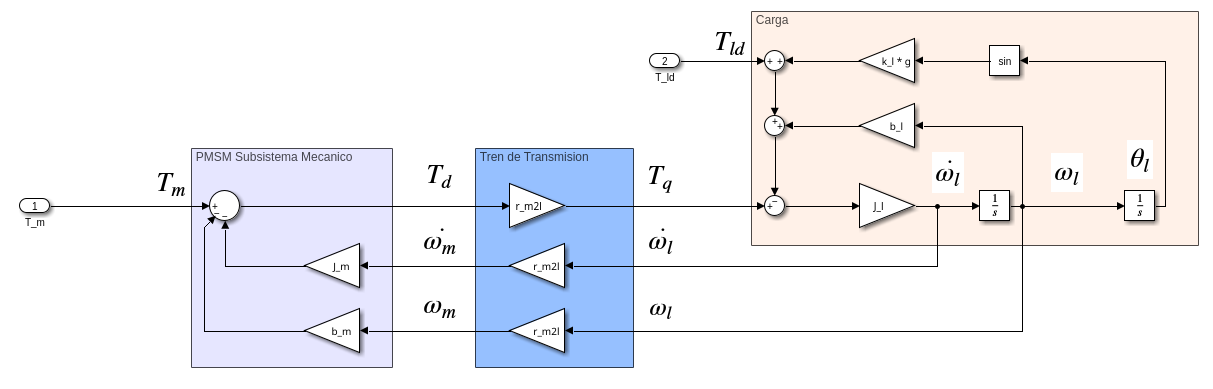
\includegraphics[width=\columnwidth]{attachments/Sistema_Carga_Trasmision_SubMecPMSM.png}
    \caption{Grafo de los sistemas de Carga, Transmisión y Subsistema Mecánico}
\end{figure}

Utilizando las ecuaciones \ref{eq:carga1} y \ref{SubMec1} se puede encontrar un reemplazo para el torque $T_d$ y pasar de un sistema de 6 ecuaciones diferenciales acopladas de primer grado a un sistema de 2 ecuaciones diferenciales de primer grado desacopladas. 

Partiendo de la ecuación \ref{eq:carga1} y despejando $T_q$ se puede llegar a la expresión:
\[
T_{q}(t) = J_{l} \frac{d\omega_{l}(t)}{dt} + b_{l}\omega_{l}(t) + k_{l}g\sin \big(\theta_{l}(t)\big) +T_{dl}(t)
\]

Se realizan los reemplazos $\omega_l=\frac{1}{r}\omega_m$, $\theta_l=\frac{1}{r}\theta_m$ y $T_q=r \; T_d$ y se reemplaza $T_d$ en la ecuación $\eqref{SubMec1}$, dejando:

\[
J_{m} \frac{d\omega_{m}(t)}{dt} = T_{m}(t) - b_{m}\omega_{m}(t) - \frac{1}{r} \left[ \frac{J_{l}}{r} \frac{d\omega_{m}(t)}{dt} + \frac{b_{l}}{r} \omega_{m}(t) + k_{l} g \sin \left( \frac{1}{r} \theta_{m}(t) \right) + T_{dl}(t) \right]
\]

Despejando, se puede llegar a:

\[
\underbrace{ \left( J_{m}+\frac{J_{l}}{r^{2}} \right)  }_{ J_{eq} } \frac{d\omega_{m}(t)}{dt} = T_{m}(t) - \underbrace{ \left( b_{m} + \frac{b_{l}}{r^{2}} \right) }_{ b_{eq} }  \omega_{m}(t) -  \frac{1}{r} T_{dl}(t)  - \frac{k_{l}g}{r} \sin \left(  \frac{1}{r} \theta_{m}(t) \right)
\]

Definimos entonces como parámetros equivalentes a:

\begin{itemize}
    \item$J_{eq}$: Momento de Inercia Equivalente del Sistema Mecánico Equivalente.
    \item$b_{eq}$: Amortiguamiento Viscoso Equivalente del Sistema Mecánico Equivalente.
\end{itemize}

\begin{table}[htbp]
    \centering
    \caption{Parámetros Equivalentes del Sistema Mecánico Equivalente}
    \small
    \begin{tabular}{lcc}
        \hline
        \textbf{Parámetro Equivalente} & \textbf{Valor} & \textbf{Magnitud (Unidad)} \\
        \hline
        $J_{eq}$ & $45.826 \times 10^{-6}$ & $\mathrm{\mathrm{kg \; m^2}}$ \\
        $b_{eq}$ & $21.944 \times 10^{-6}$ & $\mathrm{\mathrm{\frac{Nm}{rad/s}}}$ \\
        \hline
    \end{tabular}
\end{table}

\newpage
Con esta ecuación, el grafo que representa a todos los fenómenos mecánicos y su sistema de ecuaciones diferenciales respectivo es:

\begin{equation*}
    \begin{cases} % Inicia la llave grande
    \begin{aligned}
        \begin{bmatrix} \frac{d\theta_{m}(t)}{dt} \\ \frac{d\omega_{m}(t)}{dt} \end{bmatrix} &= 
        \begin{bmatrix} 0 & 1 \\ 0 & -\frac{b_{eq}}{J_{eq}} \end{bmatrix} 
        \begin{bmatrix} \theta_{m}(t) \\ \omega_{m}(t) \end{bmatrix} + 
        \begin{bmatrix} 0 \\ -\frac{k_{l}g}{r J_{eq}} \end{bmatrix} \sin \left( \frac{\theta_{m}(t)}{r} \right) + 
        \frac{1}{J_{eq}} \begin{bmatrix} 0 & 0 \\ 1 & -\frac{1}{r} \end{bmatrix} 
        \begin{bmatrix} T_{m}(t) \\ T_{ld}(t) \end{bmatrix} \\[10pt]
        \mathbf{y}(t) &= \begin{bmatrix} \theta_{m}(t) \\ \omega_{m}(t) \end{bmatrix}
    \end{aligned}
    \end{cases}
\end{equation*}



\begin{figure}[htbp]
    \centering
    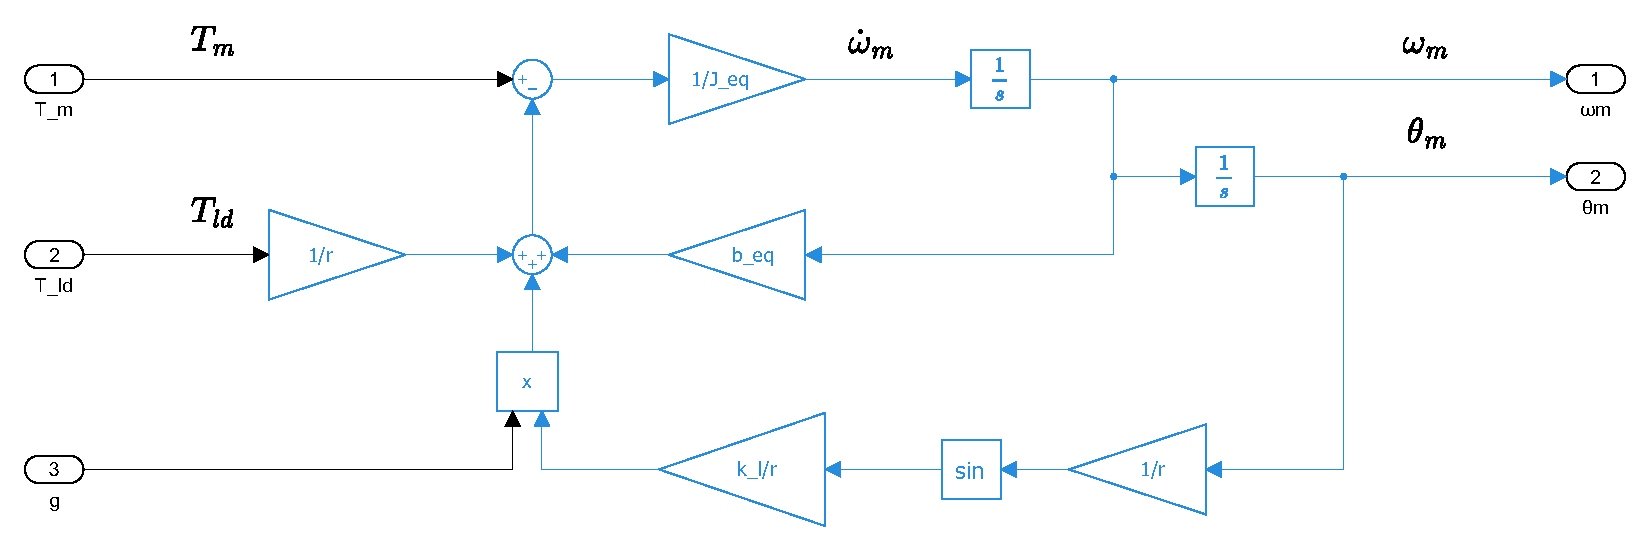
\includegraphics[width=\columnwidth]{attachments/Subsistema Mecanico Equivalente (2).pdf}
    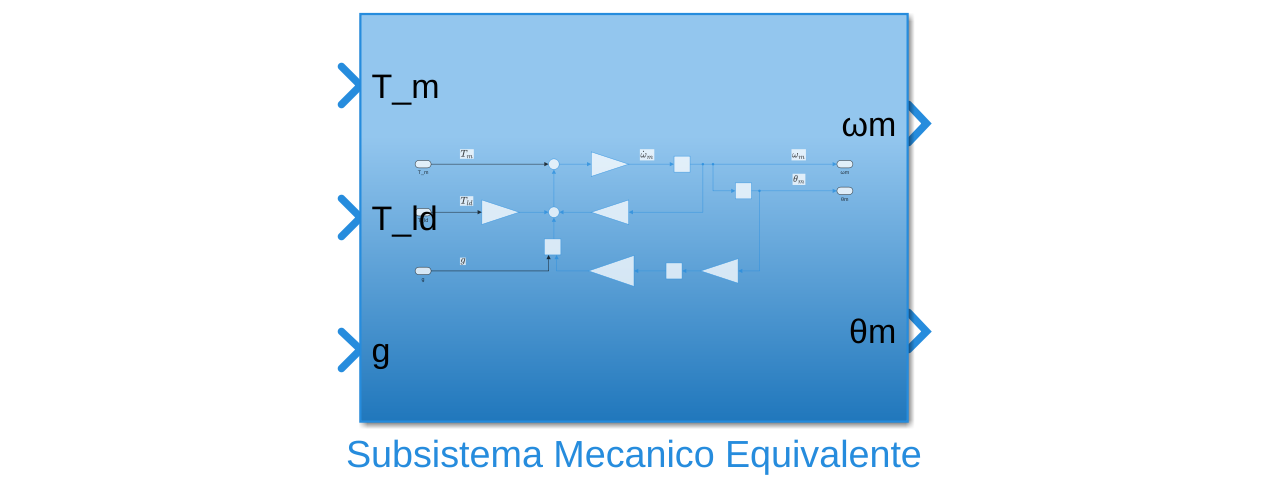
\includegraphics[width=\columnwidth]{attachments/Bloque Subsistema Mecanico Equivalente.png}
    \caption{Grafo y Bloque del Sistema Mecánico Equivalente}
\end{figure}




% ---------------------------------------------------------------------------- %
\subsection{Modelo Dinámico del Sistema Físico Completo}

% ---------------------------------------------------------------------------- %
\subsubsection{Modelo Global No Lineal}
Combinando el Sistema Mecánico Equivalente desarrollado en el inciso anterior junto con los demás sistemas de la PMSM — los previamente definidos como "Subsistema Electromagnético" y "Subsistema Térmico" respectivamente — se llega al \textbf{Modelo Global No Lineal}.

Dicha no linealidad es resultado de expresiones sinusoidales (e.g. $\sin \left( \frac{1}{r} \theta_m(t) \right)$), funciones incógnitas elevadas al cuadrado (e.g. $i_{ds}^{r \; 2}(t)$) y debido al uso de parámetros con valores locales (e.g. $b_l$). 

El Subsistema Electromagnético se desarrolla maniobrando con las corrientes virtuales de Park.  El bloque del subsistema electromagnético de la PMSM se desarrolla con las ecuaciones \ref{SubElec3}, \ref{SubElec4}, \ref{SubElec5} y \ref{SubElec6} y se despejan los términos de derivadas de las corrientes del espacio de Park para llegar a:

\begin{equation*}
\begin{cases} % Inicia la llave grande
\begin{aligned}
        T_{m}(t) &  = \frac{3}{2}P_{p} \lambda_{m}^{'r} i_{qs}^{r}(t) + \frac{3}{2} P_{p} \Big( L_{d} - L_{q} \Big) i_{qs}^{r}(t) i_{ds}^{r}(t)  \\
        \frac{di_{ds}^{r}(t)}{dt} & = \frac{1}{L_{d}} \left[ v_{ds}^{r}(t) - R_{s} \Big( T_{s}^{\circ} (t) \Big) i_{ds}^{r}(t) + L_{q}i_{qs}^{r}(t) \omega_{r}(t)  \right]  \\
        \frac{di_{qs}^{r}(t)}{dt}  & = \frac{1}{L_{q} } \left[ v_{qs}^{r}(t) - R_{s} \Big( T_{s}^{\circ} (t) \Big) i_{qs}^{r}(t) - \big[ \lambda_{m}^{'r} + L_{d} i_{ds}^{r}(t) \big] \omega_{r}(t) \right]  \\
        \frac{di_{0s}^{r}(t)}{dt} & = \frac{1}{ L_{ls} } \left[ v_{0s}^{r}(t) - R_{s} \Big( T_{s}^{\circ} (t) \Big) i_{0s}^{r}(t) \right]
\end{aligned}
\end{cases}
\end{equation*}

\begin{figure}[htbp]
    \centering
    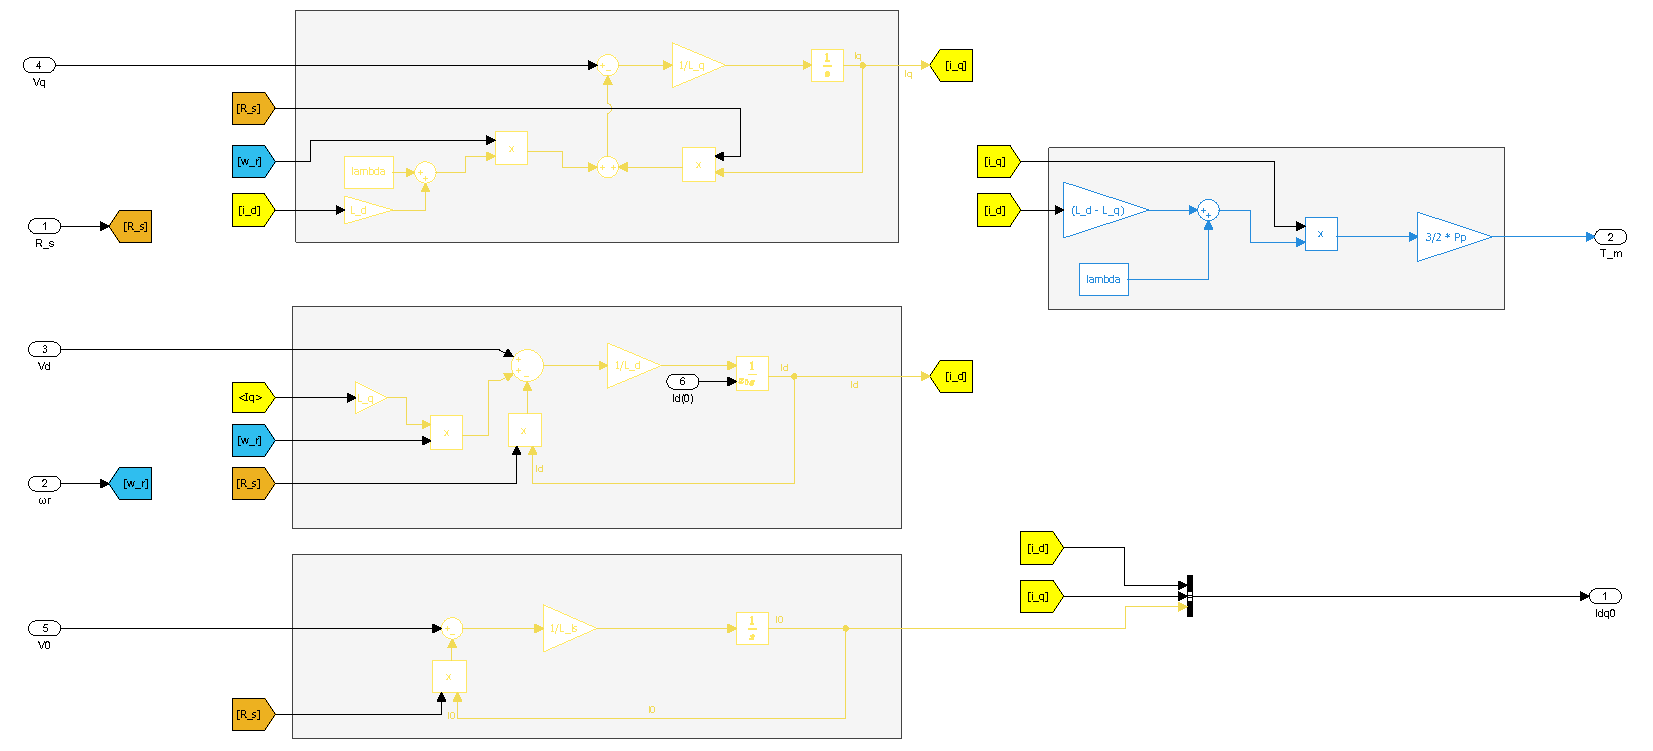
\includegraphics[width=\columnwidth]{attachments/Subsistema Electromagnetico.pdf}
    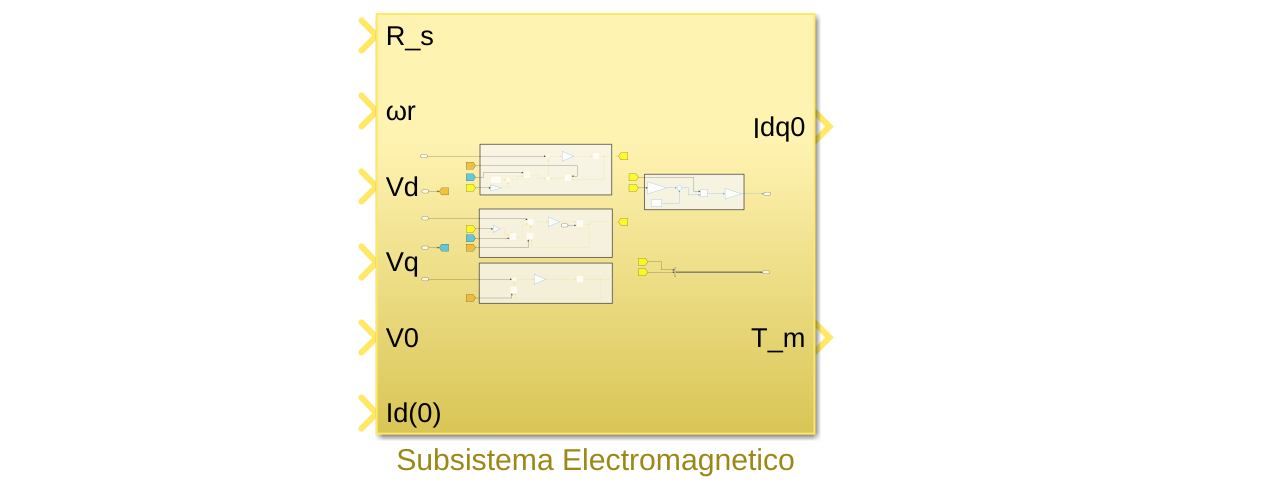
\includegraphics[width=\columnwidth]{attachments/Bloque Subsistema Electromagnetico.png}
    \caption{Grafo y Bloque del Subsistema Electromagnético de la PMSM}
\end{figure}

El planteo del subsistema térmico de la máquina PMSM se plantea como un sistema de primer orden con la diferencia de temperaturas y la potencia emanada por el motor. Además, la potencia de pérdida considera es aquella producida únicamente por efecto Joules en el bobinado del estator, despreciándose la pérdida magnética por histéresis del núcleo del motor.

Para el subsistema térmico, se hacen uso de las ecuaciones (?) y (?). Primero, se despeja la derivada de la temperatura:


\begin{align}
P_{s \; \text{perdida}}(t)  & = C_{ts} \frac{dT_{s}^{\circ}(t)}{dt} + \frac{1}{R_{ts-amb}} (T_{s}^{\circ}(t) - T_{amb}^{\circ}(t))  \\
\frac{dT_{s}^{\circ}(t)}{dt} & = \frac{1}{C_{ts}} \Bigg[ P_{s \; \text{perdida}}(t) - \frac{T_{s}^{\circ}(t) - T_{amb}^{\circ}(t)}{R_{ts-amb}} \Bigg]
\end{align}

Luego, se realiza el reemplazo $P_{s \; \text{perdida}}(t) = R_{s}(T_{s}^{\circ}(t)) \frac{3}{2} \Big( i_{qs}^{r\;2}(t) + i_{ds}^{r\;2}(t) + 2i_{0s}^{r\;2}(t) \Big)$ para considerar las corrientes del espacio de Park, debido a que el subsistema electromagnético se refiere a las corrientes de Park (fueron definidas como variables de estado), lo que deja la dinámica de la temperatura expresada como:

\begin{equation*}
    \frac{dT_{s}^{\circ}(t)}{dt} = \frac{1}{C_{ts}} \Bigg[ R_{s}(T_{s}^{\circ}(t)) \frac{3}{2} \Big( i_{qs}^{r\;2}(t) + i_{ds}^{r\;2}(t) + 2i_{0s}^{r\;2}(t) \Big) - \frac{T_{s}^{\circ}(t) - T_{amb}^{\circ}(t)}{R_{ts-amb}} \Bigg]
\end{equation*}

Adicionalmente, se considera la variación lineal de la resistencia del estator. Si bien la resistencia del estator $R_s$ no conforma una variable de estado como tal, es importante realizar el cálculo constante de su variación, debido a que influye en la dinámica de las corrientes de Park y la velocidad angular, las cuales si son variables de estado. La ecuación utilizada será:

\begin{equation*}
    R_{s}(T_{s}^{\circ}(t))  = R_{sREF} \Big(1 + \alpha_{Cu} (T_{s}^{\circ}(t) - T_{sREF}^{\circ}) \Big)
\end{equation*} 
\begin{figure}[htbp]
    \centering
    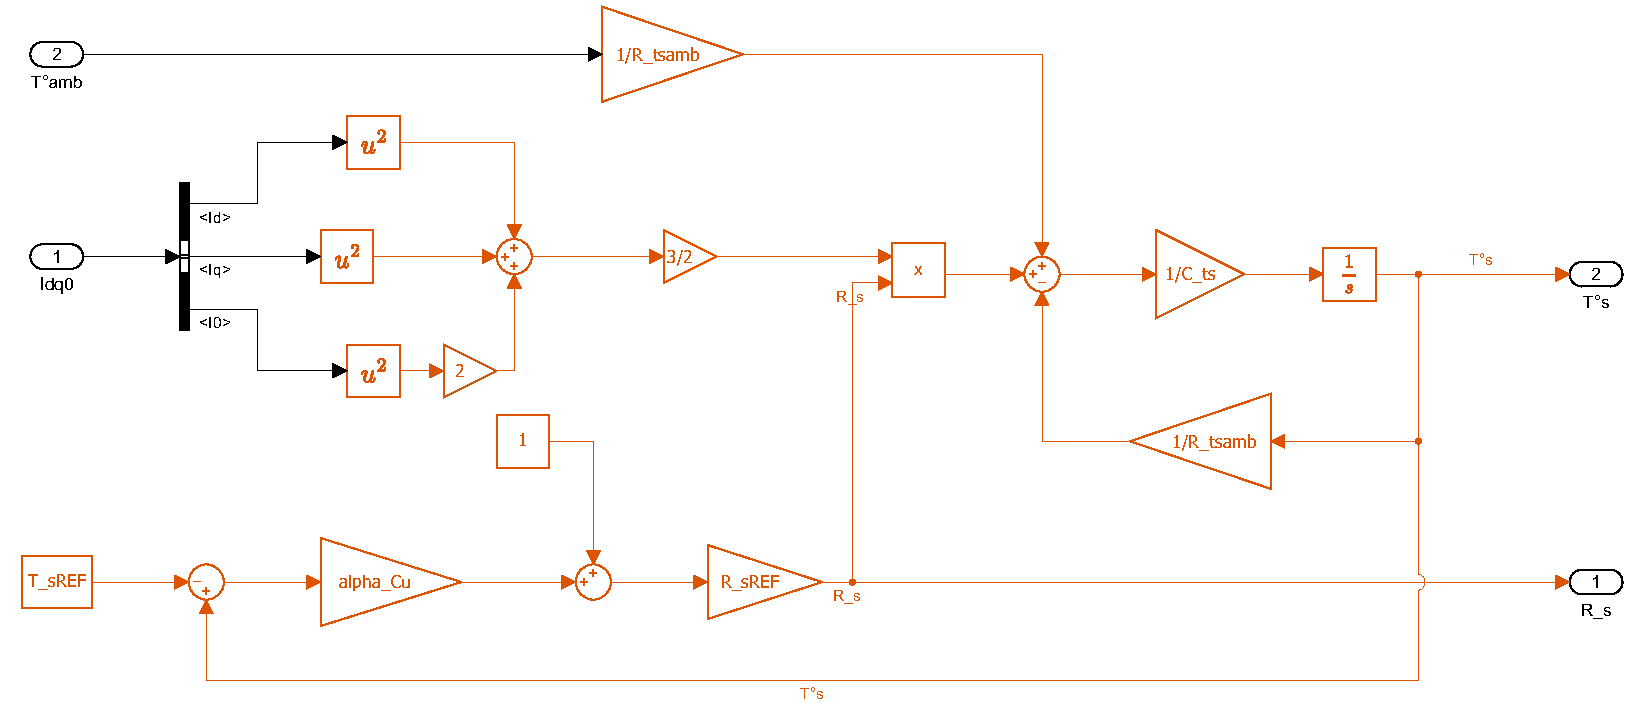
\includegraphics[width=0.9\columnwidth]{attachments/Subsistema Termico.pdf}
        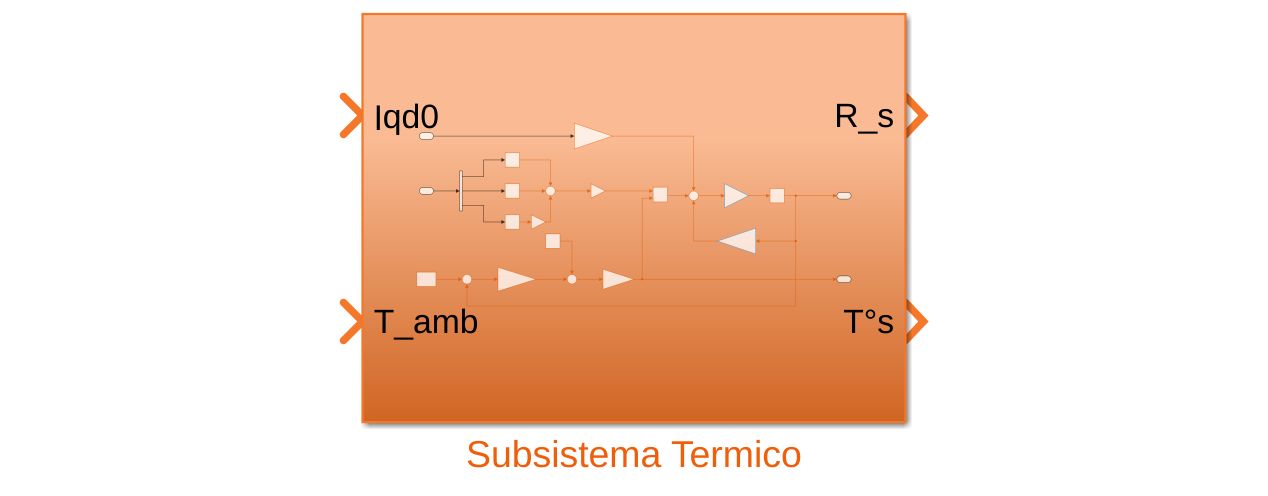
\includegraphics[width=\columnwidth]{attachments/Bloque Subsistema Termico.png}
    \caption{Grafo del Subsistema Térmico de la PMSM}
\end{figure}

\newpage
Finalmente, el Modelo Global No Lineal será el resultado de acoplar los sistemas Mecánico Equivalente, Térmico y Electromagnético, esto queda tal que:

\begin{figure}[htbp]
    \centering
    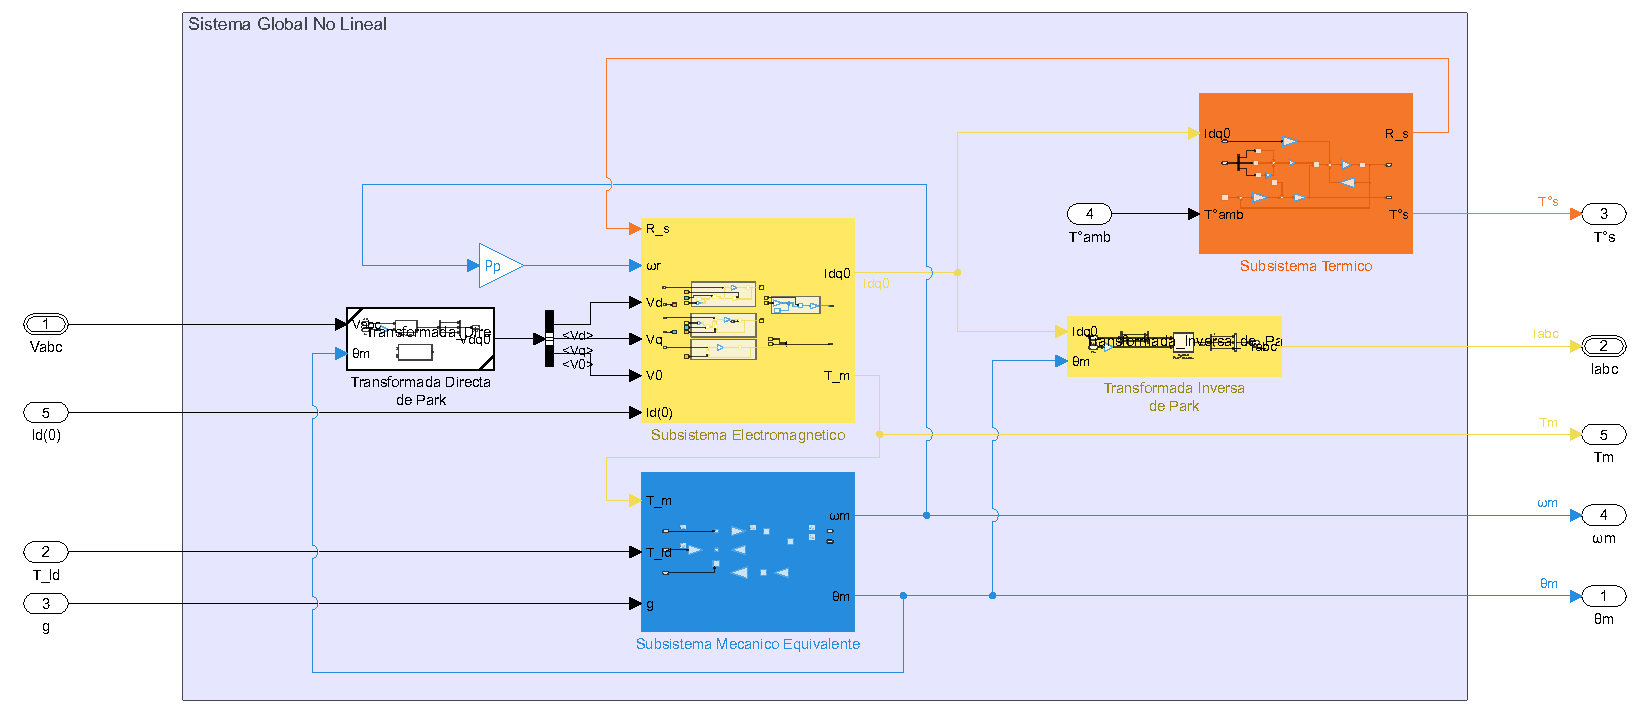
\includegraphics[width=\columnwidth]{attachments/Bloque Modelo Global No Lineal.pdf}
    \caption{Grafo del Modelo Global No Lineal}
\end{figure}

Luego, el Modelo Global No Lineal expresado en el espacio de estado puede ser expresado con el siguiente sistema de ecuaciones diferenciales no lineales de primer orden acopladas:

\begin{equation*}
    \begin{cases} % Inicia la llave grande
    \begin{aligned}
        \frac{d\theta_m(t)}{dt} & = \omega_m(t) \\
        \frac{d\omega_{m}(t)}{dt} & = \frac{1}{J_{eq}} \Bigg[ \frac{3}{2}P_{p} \lambda_{m}^{'r} i_{qs}^{r}(t) + \frac{3}{2} P_{p} \Big( L_{d} - L_{q} \Big) i_{qs}^{r}(t) i_{ds}^{r}(t) - b_{eq}  \omega_{m}(t)   - \frac{1}{r} T_{dl}(t) - \frac{k_{l}g}{r} \sin \left(  \frac{1}{r} \theta_{m}(t) \right) \Bigg]  \\
        \frac{di_{ds}^{r}(t)}{dt} & = \frac{1}{L_{d}} \left[ v_{ds}^{r}(t) - R_{s} \Big( T_{s}^{\circ} (t) \Big) i_{ds}^{r}(t) + L_{q}i_{qs}^{r}(t) \omega_{m}(t)P_{p}  \right]  \\
        \frac{di_{qs}^{r}(t)}{dt} &   = \frac{1}{L_{q} } \left[ v_{qs}^{r}(t) - R_{s} \Big( T_{s}^{\circ} (t) \Big) i_{qs}^{r}(t) - \big[ \lambda_{m}^{'r} + L_{d} i_{ds}^{r}(t) \big] \omega_{m}(t)P_{p} \right]  \\
        \frac{di_{0s}^{r}(t)}{dt} & = \frac{1}{ L_{ls} } \left[ v_{0s}^{r}(t) - R_{s} \Big( T_{s}^{\circ} (t) \Big) i_{0s}^{r}(t) \right] \\
        \frac{dT_{s}^{\circ}(t)}{dt} & = \frac{1}{C_{ts}} \Bigg[ \frac{3}{2} R_{s}\Big( T_{s}^{\circ}(t) \Big) \Big( i_{q}^{2}(t) + i_{d}^{2}(t) + 2i_{0}^{2}(t) \Big) - \frac{1}{R_{ts-amb}} \Big( T_{s}^{\circ}(t) - T_{amb}^{\circ}(t) \Big) \Bigg]
    \end{aligned}
    \end{cases}
\end{equation*}

Se definen los vectores de estado, control y perturbaciones tal que:

\begin{equation*}
    \mathbf{x}(t)= \begin{bmatrix} \theta_{m}(t) \\ \omega_{m}(t) \\ i_{ds}^{r}(t) \\ i_{qs}^{r}(t) \\ i_{0s}^{r}(t) \\ T_{s}^{\circ}(t) \end{bmatrix}, \qquad \mathbf{u}=\begin{bmatrix} v_{ds}^{r}(t) \\ v_{qs}^{r}(t) \\ v_{0s}^{r}(t) \end{bmatrix}, \qquad \mathbf{d} = \begin{bmatrix} T_{ld}(t) \\ T_{amb}^{\circ}(t)  \end{bmatrix}
\end{equation*}

Debido a las fuertes no linealidades (productos entre corrientes virtuales, producto entre una corriente virtual y la velocidad del motor, funciones sinusoidales compuestas, cuadrados de corrientes virtuales) el sistema no puede ser expresado de la forma estándar $\dot{\mathbf{x}}= \mathbf{A} \mathbf{x} + \mathbf{B} \mathbf{u}$ debido a que existen operaciones incompatibles con los productos matriciales (e.g. producto entre 2 elementos del vector $\mathbf{x}$).

En cambio, el sistema debe ser expresado como $\dot{\mathbf{x}}= f (\mathbf{x}, \mathbf{u}, \mathbf{d})$, esto es:

\begin{equation*}
    \begin{cases} % Inicia la llave grande
\begin{aligned}
\begin{bmatrix} \frac{d \theta_{m}(t) }{dt}  \\
\frac{d \omega_{m}(t) }{dt}  \\
\frac{d i_{ds}^{r}(t) }{dt} \\
\frac{d i_{qs}^{r}(t) }{dt}  \\
\frac{d i_{0s}^{r}(t) }{dt}  \\
\frac{d T_{s}^{\circ}(t) }{dt}  
\end{bmatrix} 
 & = 
\begin{bmatrix}  
\omega_m(t)   \\
\frac{1}{J_{eq}} \Bigg[ \frac{3}{2}P_{p} \lambda_{m}^{'r} i_{qs}^{r}(t) + \frac{3}{2} P_{p} \Big( L_{d} - L_{q} \Big) i_{qs}^{r}(t) i_{ds}^{r}(t) - b_{eq}  \omega_{m}(t)   - \frac{1}{r} T_{dl}(t) - \frac{k_{l}g}{r} \sin \left(  \frac{1}{r} \theta_{m}(t) \right) \Bigg]  \\
\frac{1}{L_{d}} \left[ v_{ds}^{r}(t) - R_{s} \Big( T_{s}^{\circ} (t) \Big) i_{ds}^{r}(t) + L_{q}i_{qs}^{r}(t) \omega_{m}(t)P_{p}  \right]   \\
\frac{1}{L_{q} } \left[ v_{qs}^{r}(t) - R_{s} \Big( T_{s}^{\circ} (t) \Big) i_{qs}^{r}(t) - \big[ \lambda_{m}^{'r} + L_{d} i_{ds}^{r}(t) \big] \omega_{m}(t)P_{p} \right]  \\
\frac{1}{ L_{ls} } \left[ v_{0s}^{r}(t) - R_{s} \Big( T_{s}^{\circ} (t) \Big) i_{0s}^{r}(t) \right] \\
\frac{1}{C_{ts}} \Bigg[ R_{s}(T_{s}^{\circ}(t)) \frac{3}{2} \Big( i_{qs}^{r\;2}(t) + i_{ds}^{r\;2}(t) + 2i_{0s}^{r\;2}(t) \Big) - \frac{T_{s}^{\circ}(t) - T_{amb}^{\circ}(t)}{R_{ts-amb}} \Bigg] \end{bmatrix}  \\
 \\
\mathbf{y}  & = \begin{bmatrix}
1 & 0 & 0 & 0 & 0 & 0 \\
0 & 0 & 0 & 0 & 0 & 0 \\
0 & 0 &  \sin \big( P_{p}\theta_{m}(t) \big) & \cos \big( P_{p}\theta_{m}(t) \big)  & 1 & 0 \\
0 & 0 & \sin \big( P_{p}\theta_{m}(t) - \frac{2\pi}{3} \big) & \cos \big( P_{p}\theta_{m}(t) - \frac{2\pi}{3} \big) & 1 & 0 \\
0 & 0  & \sin \big( P_{p}\theta_{m}(t) + \frac{2\pi}{3} \big) & \cos \big( P_{p}\theta_{m}(t) + \frac{2\pi}{3} \big) & 1 & 0  \\
0 & 0 & 0 & 0 & 0 & 1
\end{bmatrix} \begin{bmatrix} \theta_{m}(t) \\ \omega_{m}(t) \\ i_{ds}^{r}(t) \\ i_{qs}^{r}(t) \\ i_{0s}^{r}(t) \\ T_{s}^{\circ}(t) \end{bmatrix}
\end{aligned}
\end{cases}
\end{equation*}

Se puede armar la matriz $\mathbf{C}$ de variables de salida en base a los sensores disponibles: se tiene un sensor de posición angular incremental (encoder), un sensor de temperatura (e.g. RTD) y 3 sensores de corrientes (amperímetros) para las corrientes reales $i_{a}(t), i_{b}(t), i_{c}(t)$. Debido a que se eligieron como variables de estado a las corrientes virtuales en vez de las corrientes reales, para obtener la salida se debe aplicar la Transformada Inversa de Park, el cual viene representado por las funciones trigonométricas en función del ángulo eléctrico. Para mantener consistencia, se reemplaza el ángulo eléctrico por el ángulo motor $\theta_{r}(t) = P_{p} \theta_{m}(t)$.

% ---------------------------------------------------------------------------- %
\subsubsection{Linealización Jacobiana: Modelo global linealizado con parámetros variables (LPV)}
Recordando que el sistema presenta fuertes no linealidades, se procede a linealizar al sistema para poder analizarlo dinamicamente, se busca obtener el modelo global linealizado con parámetros variables (LPV). En el desarrollo se contempla el caso general donde $\mathbf{i_{ds}^{r}}\neq0$, a partir del modelo no lineal (NL) mediante aproximación con de serie de Taylor, en este caso la serie de Taylor se ve truncada al primer orden en un punto genérico de operación.  

Se asume que para todas las variables del modelo cumplen la forma: 
$\mathbf{z(t)}=\mathbf{Z_0(t)}+\Delta\mathbf{z(t)}$ 

Esto representa que cada variable $\mathbf{z(t)}$ se descompone en una componente de con una dependencia lenta del tiempo, no lineal pero cuasi-estacionaria  $\mathbf{Z_0(t)}$ y una componente $\Delta\mathbf{z(t)}$ dinámica lineal con una dependencia rápida del tiempo que representa las variaciones alrededor de los puntos de equilibrio.

Los puntos de equilibrio son aquellos puntos $\mathbf{(x_e, u_e,d_e)}$ en los que el sistema $\dot{\mathbf{x}}= f (\mathbf{x}, \mathbf{u}, \mathbf{d})$ cumple que $f(x_e,u_e,d_e)=0 $, lo que se alcanza cuando las variaciones de energía se han estabilizado y no hay mas movimiento o el movimiento es uniforme.
A todos los conjuntos de valores que cumplen con ser puntos de equilibrio se los denomina puntos de operación $\mathbf{\{X_0, U_0,D_0}\}$ los cuales pueden ser constantes o presentar leves variaciones uniformes con el tiempo siendo estas cuasiestacionarias, que se expresan de la siguiente forma $\mathbf{\{X_0(t), U_0(t),D_0(t)\}}$

Así el sistema NL queda expresado como sigue:

\[
\begin{cases}
\begin{aligned}
    \mathbf{\dot{x}} &\equiv \mathbf{\frac{dX_0}{dt} + \frac{d\Delta x}{dt}} \\
    & = \mathbf{f(X_0(t)+\Delta x(t), U_0(t)+\Delta u(t), D_0(t)+\Delta d(t))} \\
    
\end{aligned}
\end{cases} \qquad X_0(0) = x_0, \quad \Delta x_0(0)=0
\]

Se aproxima mediante la serie de Taylor truncada al primer orden (despreciando terminos de orden superior):
\\
\[
\dot{\mathbf{x}}(t) \approx f(\mathbf{X}_o(t), \mathbf{U}_o(t),\mathbf{D_0(t)}) + \left.\frac{\partial f}{\partial \mathbf{x}}\right|_{\mathbf{X}_o(t),\mathbf{U}_o(t),\mathbf{D}_0(t)} \Delta\mathbf{x}(t) + \left.\frac{\partial f}{\partial \mathbf{u}}\right|_{\mathbf{X}_o(t),\mathbf{U}_o(t),\mathbf{D}_0(t)} \Delta\mathbf{u}(t)+\left.\frac{\partial f}{\partial \mathbf{d}}\right|_{\mathbf{X}_o(t),\mathbf{U}_o(t),\mathbf{D}_0(t)} \Delta\mathbf{d}(t)
\]

 
Ahora se puede separar al modelo en dos partes: uno es el espacio global de puntos de operación
$X_0(t)$ denominado modelo NL cuasi-estacionario y otro es modelo dinámico local de pequeñas
desviaciones alrededor de los puntos de operación $X_0(t)$. Aquí podemos destacar que en el caso de
que el punto de operación se defina, se tratara de un sistema LTI, mientras que si varia, se tratara de un sistema LTV. \\
El espacio global de puntos de operación se obtiene de la solución del sistema de ecuaciones no lineales definido por:

\[
\dot{X}_0(t)=f(X_0(t), U_0(t), D_0(t))\approx Const; \qquad X_0(0)=x_0
\]

El cual aplicado queda:


\resizebox{\textwidth}{!}{ $\displaystyle
\begin{aligned}
\begin{bmatrix}
    \frac{d\theta_{m-0}(t)}{dt} \\[2mm]
    \frac{d\omega_{m-0}(t)}{dt} \\[2mm]
    \frac{di_{ds-0}^{r}(t)}{dt} \\[2mm]
    \frac{di_{qs-0}^{r}(t)}{dt} \\[2mm]
    \frac{di_{0s-0}^{r}(t)}{dt} \\[2mm]
    \frac{dT_{s-0}^{\circ}(t)}{dt}
\end{bmatrix} 
&= 
\begin{bmatrix}
    \omega_m(t) \\[2mm]
    \frac{1}{J_{eq}} \Bigg[ \frac{3}{2}P_{p}\Big( \lambda_{m}^{'r} + ( L_{d} - L_{q} ) i_{ds-0}^{r}(t)\Big)i_{qs-0}^{r}(t)  - \frac{T_{dl-0}(t)}{r} - b_{eq}  \omega_{m-0}(t) - \frac{k_{l}g}{r} \sin \left(  \frac{1}{r} \theta_{m-0}(t) \right) \Bigg] \\[2mm]
    \frac{1}{L_{d}} \left[ v_{ds-0}^{r}(t) - R_{s} \Big( T_{s}^{\circ} (t) \Big) i_{ds-0}^{r}(t) + L_{q}i_{qs-0}^{r}(t) \omega_{m-0}(t)P_{p}  \right] \\[2mm]
    \frac{1}{L_{q} } \left[ v_{qs-0}^{r}(t) - R_{s} \Big( T_{s-0}^{\circ} (t) \Big) i_{qs-0}^{r}(t) - \big[ \lambda_{m}^{'r} + L_{d} i_{ds-0}^{r}(t) \big] \omega_{m-0}(t)P_{p} \right] \\[2mm]
    \frac{1}{ L_{ls} } \left[ v_{0s-0}^{r}(t) - R_{s} \Big( T_{s-0}^{\circ} (t) \Big) i_{0s-0}^{r}(t) \right] \\[2mm]
    \frac{1}{C_{ts}} \left( \frac{3}{2} R_s\Big( T_{s-0}^{\circ}(t) \Big) \left[ i_{qs-0}^{r \; 2}(t) + i_{ds-0}^{r \; 2}(t) + 2i_{0s-0}^{r \; 2}(t) \right] + \frac{T_{amb}^{\circ}(t) - T_{s-0}^{\circ}(t)}{R_{ts-amb}} \right)
\end{bmatrix} \\ 
&= 
\begin{bmatrix}
    \omega_{m-0} \\[2mm]
    0 \\[2mm]
    0 \\[2mm]
    0 \\[2mm]
    0 \\[2mm]
    0
\end{bmatrix}
\end{aligned}
$} 


Por otro lado el modelo dinámico local que definido por:

\[
\frac{d\Delta x}{dt}=\left.\frac{\partial f}{\partial \mathbf{x}}\right|_{\mathbf{X}_o(t),\mathbf{U}_o(t),\mathbf{D}_0(t)} \Delta\mathbf{x}(t) + \left.\frac{\partial f}{\partial \mathbf{u}}\right|_{\mathbf{X}_o(t),\mathbf{U}_o(t),\mathbf{D}_0(t)} \Delta\mathbf{u}(t)+\left.\frac{\partial f}{\partial \mathbf{d}}\right|_{\mathbf{X}_o(t),\mathbf{U}_o(t),\mathbf{D}_0(t)} \Delta\mathbf{d}(t) \quad ; \qquad \Delta x_0(0)=0
\]

Donde:

\begin{equation*}
\Delta \mathbf{x}(t)=\begin{bmatrix}
    \Delta \theta_{m}(t) \\[2mm]
    \Delta \omega_{m}(t) \\[2mm]
    \Delta i_{ds}^{r}(t) \\[2mm]
    \Delta i_{qs}^{r}(t)\\[2mm]
    \Delta i_{0s}^{r}(t) \\[2mm]
    \Delta T_{s}^{\circ}(t)
\end{bmatrix},\qquad 
\Delta \mathbf{u}(t)=\begin{bmatrix} \Delta v_{ds}^{r}(t) \\ \Delta v_{qs}^{r}(t) \\ \Delta v_{0s}^{r}(t) \end{bmatrix}, \qquad 
\Delta \mathbf{d}(t) = \begin{bmatrix} \Delta T_{ld}(t) \\ \Delta T_{amb}^{\circ}(t)  \end{bmatrix}
\end{equation*}

y

\begin{align*}
\left. \frac{\partial f}{\partial \mathbf{x}} \right|_{\mathbf{x}_0(t), \mathbf{U}_0(t), \mathbf{D}_0(t)}  & = \left. \frac{\partial f}{\partial \mathbf{x}} \right|_o = \begin{bmatrix} \left. \frac{\partial f}{\partial \theta_m} \right|_o & \left. \frac{\partial f}{\partial \omega_m} \right|_o & \left. \frac{\partial f}{\partial i_{ds}^r} \right|_o &  \left. \frac{\partial f}{\partial i_{qs}^r} \right|_o  & \left. \frac{\partial f}{\partial i_{0s}^r} \right|_o & \left. \frac{\partial f}{\partial T_s^{\circ}} \right|_o \end{bmatrix} \\
\left. \frac{\partial f}{\partial \mathbf{u}} \right|_{\mathbf{x}_0(t), \mathbf{U}_0(t), \mathbf{D}_0(t)}  & = \left. \frac{\partial f}{\partial \mathbf{u}} \right|_o = \begin{bmatrix} \left. \frac{\partial f}{\partial v_{ds}^{r}} \right|_o & \left. \frac{\partial f}{\partial v_{qs}^{r}} \right|_o & \left. \frac{\partial f}{\partial v_{0s}^{r}} \right|_o \end{bmatrix} \\
\left. \frac{\partial f}{\partial \mathbf{d}} \right|_{\mathbf{x}_0(t), \mathbf{U}_0(t), \mathbf{D}_0(t)}  & = \left. \frac{\partial f}{\partial \mathbf{d}} \right|_o = \begin{bmatrix} \left. \frac{\partial f}{\partial T_{ld}} \right|_o & \left. \frac{\partial f}{\partial T_{amb}^{\circ}} \right|_o \end{bmatrix}
\end{align*}

pero se reordena uniendo entradas de control (\(\mathbf{u}\)) y entradas de perturbación (\(\mathbf{d}\)) en entradas en general, quedando como sigue:

\[
\left. \frac{\partial f}{\partial \mathbf{u}} \right|_{\mathbf{x}_0(t), \mathbf{U}_0(t), \mathbf{D}_0(t)} = \left. \frac{\partial f}{\partial \mathbf{u}} \right|_o = \begin{bmatrix} \left. \frac{\partial f}{\partial v_{ds}^{r}} \right|_o & \left. \frac{\partial f}{\partial v_{qs}^{r}} \right|_o & \left. \frac{\partial f}{\partial v_{0s}^{r}} \right|_o \left.  \frac{\partial f}{\partial T_{ld}} \right|_o & \left. \frac{\partial f}{\partial T_{amb}^{\circ}} \right|_o \end{bmatrix}
\]

\[
\Delta \mathbf{u}(t)=\begin{bmatrix} \Delta v_{ds}^{r}(t) \\ \Delta v_{qs}^{r}(t) \\ \Delta v_{0s}^{r}(t) \\\Delta T_{ld}(t) \\ \Delta T_{amb}^{\circ}(t)\end{bmatrix}
\]

Queda finalmente:


\resizebox{\textwidth}{!}{
$\displaystyle
\frac{d \Delta x}{dt} = 
\begin{bmatrix}
    0 & 1 & 0 & 0 & 0 & 0 \\
    -\frac{k_{l}g}{J_{eq} \cdot r^2} \cos \left( \frac{1}{r} \theta_{m-0}(t) \right) & -\frac{b_{eq}}{J_{eq}} & \frac{1}{J_{eq}}\frac{3}{2} P_{p} \Big( L_{d} - L_{q} \Big) i_{qs-0}^{r} & \frac{1}{J_{eq}} \frac{3}{2}P_{p}\Big( \lambda_{m}^{'r} + \Big( L_{d} - L_{q} \Big) i_{ds-0}^{r}(t)\Big) & 0 & 0 
    \\
    0 & \frac{L_{q}i^r_{qs-0}P_p}{L_d} & \frac{-R_s(T^\circ_{s-0})}{L_d} & \frac{L_q \omega_{m-0}P_p}{{L_d}} & 0 &  -\frac{\alpha_{Cu} R_{sREF}}{L_d} i_{ds-0}^{r}(t) 
    \\
    0 & -\frac{P_{p}[\lambda_{m}^{'r} + L_{d} i_{ds-0}^{r}(t)]}{L_q} & -\frac{L_d \omega_{m-0}P_p}{L_q} & \frac{-R_s(T^\circ_{s-0})}{L_q} & 0 & -\frac{\alpha_{Cu} R_{sREF}}{L_q} i_{qs-0}^{r}(t) 
    \\
    0 & 0 & 0 & 0 & \frac{-R_s(T^\circ_{s-0})}{L_{ls}} & -\frac{\alpha_{Cu} R_{sREF}}{L_{ls}} i_{0s-0}^{r}(t) 
    \\
    0 & 0 & \frac{3}{C_{ts}} R_s\Big( T_{s-0}^{\circ}(t) \Big) i_{ds-0}^{r}(t) & \frac{3}{C_{ts}} R_s\Big( T_{s-0}^{\circ}(t) \Big) i_{qs-0}^{r}(t) &  \frac{6}{C_{ts}} R_s\Big( T_{s-0}^{\circ}(t) \Big) i_{0s-0}^{r}(t) & \frac{1}{C_{ts}} \left( \alpha_{Cu} R_{sREF} \frac{3}{2} \left[ i_{qs-0}^{r \; 2}(t) + i_{ds-0}^{r \; 2}(t) + 2i_{0s-0}^{r \; 2}(t) \right] - \frac{1}{R_{ts-amb}} \right)
\end{bmatrix}
\begin{bmatrix}
    \Delta \theta_{m}(t) \\[2mm]
    \Delta \omega_{m}(t) \\[2mm]
    \Delta i_{ds}^{r}(t) \\[2mm]
    \Delta i_{qs}^{r}(t)\\[2mm]
    \Delta i_{0s}^{r}(t) \\[2mm]
    \Delta T_{s}^{\circ}(t)
\end{bmatrix}
+
\begin{bmatrix}
    0 & 0 & 0 & 0 & 0 \\
    0 & 0 & 0 &  \frac{-1}{J_{eq}}\frac{1}{r} & 0\\
    \frac{1}{L_d} & 0 & 0 & 0 & 0\\
    0 & \frac{1}{L_q} & 0 & 0 & 0\\
    0 & 0 & \frac{1}{L_{ls}} & 0 & 0\\
    0 & 0 & 0 & 0 & \frac{1}{C_{ts}R_{ts-amb}}    
\end{bmatrix}
\begin{bmatrix} 
    \Delta v_{ds}^{r}(t) \\ 
    \Delta v_{qs}^{r}(t) \\ 
    \Delta v_{0s}^{r}(t) \\
    \Delta T_{ld}(t) \\ 
    \Delta T_{amb}^{\circ}(t)
\end{bmatrix}
$}




%---------------------------------------------------------------------------- %
\subsubsection{ Linealización por Retroalimentación NL: Modelo simplificado lineal invariante (LTI)
equivalente}

Previo al desarrollo del modelo simplificado lineal invariante en el tiempo (LTI), se busca tomar acciones correctivas contra las no linealidades más destacables del Modelo Global No Lineal.

Para poder diseñar un modelo linealizado a partir del Modelo Global No Lineal, primero se deben adoptan una serie de hipótesis:

\begin{enumerate}
    \item \textbf{Corriente homopolar nula.} \\
    Debido a que la máquina PMSM trabaja con conexión estrella sin acceso al neutro, por leyes de Kirchoff las corrientes \(i_a(t), i_b(t), i_c(t)\) cumplirán con la ley de nodos de Kirchoff, esto es:

    \begin{equation}
        i_a(t) + i_b(t) + i_c(t) = 0 
    \end{equation}

    Por lo que aplicar la Transformada Directa de Park, vemos que:

    \begin{equation}
        i_{0s}^{r}(t) = \frac{1}{3} \Big(  i_a(t) + i_b(t) + i_c(t)  \Big) = 0 
    \end{equation}
    
    Y la dinámica descrita por la ecuación diferencial será nula siempre que \(v_{0s}^{r}(t) = 0\):

    \begin{equation}
        v_{0s}^{r}(t) = 0 \qquad \therefore \; \frac{di_{0s}^{r}(t)}{dt}   \equiv 0   
    \end{equation}
    

    \item \textbf{Variación de la Resistencia \(R_s\)} \\
A pesar de que la resistencia del estátor varía de forma lineal con la temperatura del bobinado según $R_s(T_s^\circ(t)) = R_{sREF}[1 + \alpha_{Cu}(T_s^\circ(t) - T_{sREF}^\circ)]$, para el análisis dinámico local se adopta un valor constante parametrizado como $R_s^\ell$. Se asume que el motor opera bajo un régimen térmico cuasiestacionario en torno a una temperatura promedio de trabajo de $60^\circ\text{C}$ (un valor intermedio realista entre la temperatura ambiente y la máxima admisible de $115^\circ\text{C}$). Evaluando la variación lineal, se fija dicho parámetro constante en:
    \begin{equation*}
        R_s^\ell = R_s(60^\circ\text{C}) \approx 1{,}18\,\Omega
    \end{equation*}
Esto permite preservar la estructura del modelo lineal e invariante en el tiempo (LTI), garantizando al mismo tiempo que las pérdidas de energía estimadas y las constantes de tiempo eléctricas reales del transitorio representen adecuadamente las condiciones reales de operación en caliente.
    
    \item \textbf{Independizarse de la ecuación de la dinámica térmica} \\
El subsistema térmico presenta una constante de tiempo significativamente mayor (del orden de minutos) en comparación con las rápidas dinámicas de los transitorios electromecánicos y electromagnéticos del accionamiento (del orden de milisegundos). Debido a esta notable separación temporal de escalas, la temperatura del estátor $T_s^\circ(t)$ se comporta de forma cuasiestática frente a las perturbaciones y variaciones rápidas de la velocidad del motor y las corrientes de fase. Por consiguiente, es posible desacoplar la ecuación diferencial de la dinámica térmica del resto de las ecuaciones de estado del sistema físico, reduciendo el orden del modelo dinámico activo para el diseño de la ley de control sin incurrir en pérdidas de precisión apreciables en el transitorio eléctrico.
    
\end{enumerate}

Con estas hipótesis tomadas, se pueden aplicar leyes de control que permitan linealizar el Modelo Global No Lineal, con el afán de cumplir con la solicitud $i_{ds}^{r}(t) \equiv 0$, la cual permite realizar un desacople de los canales de flujo magnético y torque.

Primero, se analiza la dinámica de $i_{ds}^{r}(t)$,

\begin{equation*}
    \frac{di_{ds}^{r}(t)}{dt} = \frac{1}{L_{d}} \left[ v_{ds}^{r}(t) - R_{s}^{\ell} i_{ds}^{r}(t) + L_{q}P_{p} i_{qs}^{r}(t) \omega_{m}(t) \right]
\end{equation*}

donde el único término que introduce no linealidades es $ L_{q}i_{qs}^{r}(t) \omega_{m}(t)P_{p}$. Dicho término representa... 

A partir de la dinámica de la corriente directa, se pueden derivar 2 casos de interés:

\begin{enumerate}
    \item \textbf{Caso Particular: Condición Inicial Nula} $i_{ds}^{r}(t_0) = 0$ \\
    Si la corriente directa tiene valor inicial nulo, entonces se puede despreciar momentánea e inicialmente la influencia de la corriente directa, por lo que la dinámica queda tal que:

    \begin{equation*}
        \frac{di_{ds}^{r}(t)}{dt} = \frac{1}{L_{d}} \left[ v_{ds}^{r}(t) - \cancelto{0}{R_{s}^{\ell} i_{ds}^{r}(t)} + L_{q}P_{p} i_{qs}^{r}(t) \omega_{m}(t) \right]
    \end{equation*}

    Para que la corriente directa se mantenga con valor nulo $i_{ds}^{r}(t) = 0$ a partir de su valor inicial propuesto $i_{ds}^{r}(t_0) = 0$, se requiere que la derivada de la corriente directa sea nula también $\frac{di_{ds}^{r}(t)}{dt} = 0$, lo que implica inexistencia de variaciones en la corriente directa (empieza con valor nulo y no hay variaciones, ende se mantiene con valor nulo). Viendo la ecuación dinámica:

    \begin{align*}
        \frac{di_{ds}^{r}(t)}{dt} = \frac{1}{L_{d}} \left[ v_{ds}^{r}(t) - \cancelto{0}{R_{s}^{\ell} i_{ds}^{r}(t)} + L_{q}P_{p} i_{qs}^{r}(t) \omega_{m}(t) \right] & = 0 \\
        \frac{1}{L_{d}} \left[ v_{ds}^{r}(t) + L_{q}P_{p} i_{qs}^{r}(t) \omega_{m}(t) \right] & = 0 \\
         v_{ds}^{r}(t) + L_{q}P_{p} i_{qs}^{r}(t) \omega_{m}(t) & = 0
    \end{align*}

    En base a esto, se implementa una restricción o Ley de Control Mínima que impone:
    
    \begin{equation}
        v_{ds}^{r}(t)  = -L_{q}P_{p} i_{qs}^{r}(t) \omega_{m}(t)
    \end{equation}
    
    Ello permite que la dinámica de la corriente directa se mantenga nula durante el resto del tiempo de trabajo. La dinámica queda tal que:

    \begin{align*}
        \frac{di_{ds}^{r}(t)}{dt} & = \frac{1}{L_{d}} \left[v_{ds}^{r}(t) - R_{s}^{\ell} i_{ds}^{r}(t) + L_{q}P_{p} i_{qs}^{r}(t) \omega_{m}(t) \right]
        \\
        \frac{di_{ds}^{r}(t)}{dt} & = \frac{1}{L_{d}} \Big[ - \Big(  L_{q}P_{p} i_{qs}^{r}(t) \omega_{m}(t) \Big) - R_{s}^{\ell} i_{ds}^{r}(t) + L_{q}P_{p} i_{qs}^{r}(t) \omega_{m}(t) \Big]
        \\
        \frac{di_{ds}^{r}(t)}{dt} & = \frac{1}{L_{d}} \Big[ - \cancel{ \Big(  L_{q}P_{p} i_{qs}^{r}(t) \omega_{m}(t) \Big) } - R_{s}^{\ell} \cancelto{ 0 }{  i_{ds}^{r}(t) } + \cancel{ L_{q}P_{p} i_{qs}^{r}(t) \omega_{m}(t)  }\Big] = 0 \qquad \therefore \; \frac{di_{ds}^{r}(t)}{dt} \equiv 0
    \end{align*}
    
    Luego, de analizarse la dinámica de la corriente en cuadratura $i_{qs}^{r}(t)$, donde se puede apreciar que existe acoplamiento con la corriente directa $i_{ds}^{r}(t)$, y que al aplicar la Ley de Control Mínima se modifica según:

    \begin{equation*}
        \frac{di_{qs}^{r}(t)}{dt} = \frac{1}{L_{q} } \left[ v_{qs}^{r}(t) - R_{s}^{\ell} i_{qs}^{r}(t) - \big[ \lambda_{m}^{'r} +\cancel{  L_{d} i_{ds}^{r}(t) } \big] \omega_{m}(t)P_{p} \right]
    \end{equation*}

    Por lo que permite un desacople entre las corrientes directa y en cuadratura, linealizando la dinámica de la corriente en cuadratura $i_{qs}^{r}(t)$. Esta forma de linealización no es debido a que se introduce un término que cancele la expresión lineal, sino de que el término no lineal fue anulado a partir de su ecuación dinámica.
    
    La expresión resultante será:

    \begin{equation*}
        \frac{di_{qs}^{r}(t)}{dt} = \frac{1}{L_{q} } \left[ v_{qs}^{r}(t) - R_{s}^{\ell} i_{qs}^{r}(t) -\lambda_{m}^{'r} P_{p} \omega_{m}(t) \right]
    \end{equation*}

    Con la misma Ley de Control Mínima, se linealiza tanto la dinámica de la corriente directa como la dinámica de la corriente en cuadratura, siempre y cuando el valor inicial de la corriente directa sea nulo $i_{ds}^{r}(t_0) = 0$.

    \item \textbf{Caso General: Condición Inicial No Nula} $i_{ds}^{r}(t_0) \neq 0$ \\
    En el caso general donde el valor inicial de la corriente directa no es necesariamente nulo, se aprecia que la dinámica de la corriente directa adopta un comportamiento exponencial decreciente si se mantiene la misma Ley de Contro Mínima $v_{ds}^{r}(t)  = -L_{q}P_{p} i_{qs}^{r}(t) \omega_{m}(t)$, según:
    
    \begin{align*}
    \frac{di_{ds}^{r}(t)}{dt} & = \frac{1}{L_{d}} \left[v_{ds}^{r}(t) - R_{s}^{\ell} i_{ds}^{r}(t) + L_{q}P_{p} i_{qs}^{r}(t) \omega_{m}(t) \right]
    \\
    \frac{di_{ds}^{r}(t)}{dt} & = \frac{1}{L_{d}} \Big[ - \Big(  L_{q}P_{p} i_{qs}^{r}(t) \omega_{m}(t) \Big) - R_{s}^{\ell} i_{ds}^{r}(t) + L_{q}P_{p} i_{qs}^{r}(t) \omega_{m}(t) \Big]
    \\
    \frac{di_{ds}^{r}(t)}{dt} & = \frac{1}{L_{d}} \Big[ - \cancel{ \Big(  L_{q}P_{p} i_{qs}^{r}(t) \omega_{m}(t) \Big) } - R_{s}^{\ell} i_{ds}^{r}(t) + \cancel{ L_{q}P_{p} i_{qs}^{r}(t) \omega_{m}(t)  }\Big]  \\
    \frac{di_{ds}^{r}(t)}{dt} & = -\frac{1}{L_{d}} R_{s}^{\ell} i_{ds}^{r}(t) \\
     \therefore \; i_{ds}^{r}(t)  & \equiv i_{ds}^{r}(t_0) e^{ -\frac{ R_{s}^{\ell} }{L_{d}} \cdot t  }
    \end{align*}

    Entonces, la corriente directa se extingue a medida que pasa el tiempo. El problema es que durante el estado transitorio, la corriente directa sigue acoplada a la dinámica de la corriente en cuadratura y no es hasta que se estingue $i_{ds}^{r}(t)$ que la dinámica de $i_{qs}^{r}(t)$ se vuelve "independiente" de los efectos de la corriente directa.

    Para ello, se puede implementar una Ley de Control Mínima Complementaria que por retroalimentación anule el término no lineal de la corriente directa que afecta a la dinámica de la corriente en cuadratura, esto es:

    \begin{equation}
        v_{qs}^{r}(t) =   L_{d} \ P_{p} \ i_{ds}^{r}(t) \ \omega_{m}(t)
    \end{equation}

    Con este termino, se aprecia que:

    \begin{align*}
        \frac{di_{qs}^{r}(t)}{dt}  & = \frac{1}{L_{q} } \left[ v_{qs}^{r}(t) - R_{s}^{\ell} i_{qs}^{r}(t) - \lambda_{m}^{'r} P_{p}  \omega_{m}(t) -  L_{d} P_{p} i_{ds}^{r}(t) \omega_{m}(t)  \right]
        \\
        \frac{di_{qs}^{r}(t)}{dt}  & = \frac{1}{L_{q} } \left[ \Big( L_{d} P_{p} i_{ds}^{r}(t) \omega_{m}(t) \Big) - R_{s}^{\ell} i_{qs}^{r}(t) - \lambda_{m}^{'r} P_{p}  \omega_{m}(t) -  L_{d} P_{p} i_{ds}^{r}(t) \omega_{m}(t)  \right]
        \\
        \frac{di_{qs}^{r}(t)}{dt}  & = \frac{1}{L_{q} } \left[ \cancel{ \Big( L_{d} P_{p} i_{ds}^{r}(t) \omega_{m}(t) \Big) } - R_{s}^{\ell} i_{qs}^{r}(t) - \lambda_{m}^{'r} P_{p}  \omega_{m}(t) - \cancel{  L_{d} P_{p} i_{ds}^{r}(t) \omega_{m}(t) }  \right]\\
        \frac{di_{qs}^{r}(t)}{dt}  & = \frac{1}{L_{q} } \left[ - R_{s}^{\ell} i_{qs}^{r}(t) - \lambda_{m}^{'r} P_{p}  \omega_{m}(t)  \right]
    \end{align*}

    A diferencia de la Ley de Control Mínima, que ejerce control en el eje directo, la cual no linealiza por retroalimentación sino que fuerza a la dinámica de la corriente directa a que adopte una naturaleza exponencial decreciente, la Ley de Control Mínima Complementaria añade control en el eje en cuadratura (adicional al control en el eje directo), la cual si realiza una retroalimentación no lineal en la dinámica de la corriente en cuadratura que elimina el efecto no lineal $-L_{d} P_{p} i_{ds}^{r}(t) \omega_{m}(t) $ mediante la modulación de la tensión en cuadratura $ v_{qs}^{r}(t)$.

    Con el control simultáneo en el eje directo y el eje en cuadratura, se puede realizar una linealización más robusta, debido a que no se necesita imponer la condición inicial $i_{ds}^{r}(t_0) = 0$ ni depender que $i_{ds}^{r}(t)$ se extinga rápidamente para que deje de influir en la dinámica de $i_{qs}^{r}(t)$, sino que el comportamiento lineal de la corriente $i_{qs}^{r}(t_0)$ estará asegurado independientemente del valor inicial de $i_{ds}^{r}(t_0)$ o de la velocidad de decaimiento de la corriente $i_{ds}^{r}(t_0)$.
\end{enumerate}

Debido a su robustez, se implementa la Ley de Control Mínima Complementaria, lo que implica control en el eje directo y el eje en cuadratura. Con esta retroalimentación, se puede ver que el modelo linealizado no es afectado por las dinámicas de las corrientes directa ni homopolar, y al desprenderse de la dinámica térmica, se puede plantear el siguiente modelo LTI equivalente:

\[
\resizebox{\textwidth}{!}{$\displaystyle
    \text{GNL} 
    \begin{cases}
        \begin{aligned} 
            \frac{d\theta_m(t)}{dt} & = \omega_m(t) \\
            \frac{d\omega_{m}(t)}{dt} & = \frac{1}{J_{eq}} \Bigg[ \frac{3}{2}P_{p} \lambda_{m}^{'r} i_{qs}^{r}(t) + \frac{3}{2} P_{p} \Big( L_{d} - L_{q} \Big) i_{qs}^{r}(t) i_{ds}^{r}(t)  - \frac{T_{dl}(t)}{r} - b_{eq}  \omega_{m}(t) - \frac{k_{l}g}{r} \sin \left(  \frac{1}{r} \theta_{m}(t) \right) \Bigg]  \\
            \frac{di_{ds}^{r}(t)}{dt} & = \frac{1}{L_{d}} \left[ v_{ds}^{r}(t) - R_{s} \Big( T_{s}^{\circ} (t) \Big) i_{ds}^{r}(t) + L_{q}i_{qs}^{r}(t) \omega_{m}(t)P_{p}  \right] \label{variacion_ids} \\
            \frac{di_{qs}^{r}(t)}{dt}  & = \frac{1}{L_{q} } \left[ v_{qs}^{r}(t) - R_{s} \Big( T_{s}^{\circ} (t) \Big) i_{qs}^{r}(t) - \big[ \lambda_{m}^{'r} + L_{d} i_{ds}^{r}(t) \big] \omega_{m}(t)P_{p} \right]  \\
            \frac{di_{0s}^{r}(t)}{dt} & = \frac{1}{ L_{ls} } \left[ v_{0s}^{r}(t) - R_{s} \Big( T_{s}^{\circ} (t) \Big) i_{0s}^{r}(t) \right] \\
            \frac{dT_{s}^{\circ}(t)}{dt} & = \frac{1}{C_{ts}} \Bigg[ \frac{3}{2} R_{s}\Big( T_{s}^{\circ}(t) \Big) \Big( i_{q}^{2}(t) + i_{d}^{2}(t) + 2i_{0}^{2}(t) \Big) - \frac{1}{R_{ts-amb}} \Big( T_{s}^{\circ}(t) - T_{amb}^{\circ}(t) \Big) \Bigg]
        \end{aligned}
    \end{cases} 
    \implies \quad
    \begin{aligned}
        \text{LTI} \quad & 
        \begin{cases}
            \begin{aligned}
                \frac{d\theta_m(t)}{dt} & = \omega_m(t) \\
                \frac{d\omega_{m}(t)}{dt} & = \frac{1}{J_{eq}} \Bigg[ \frac{3}{2}P_{p} \lambda_{m}^{'r} i_{qs}^{r}(t) - b_{eq}  \omega_{m}(t) - T_{d}(t) \Bigg]  \\
                \frac{di_{qs}^{r}(t)}{dt}  & = \frac{1}{L_{q} } \left[ v_{qs}^{r}(t) - R_{s}^{\ell} i_{qs}^{r}(t) - \lambda_{m}^{'r}P_{p} \omega_{m}(t) \right]
            \end{aligned}
        \end{cases} \\[4mm]
        & \frac{dT_{s}^{\circ}(t)}{dt} = \frac{1}{C_{ts}} \Bigg[ \frac{3}{2} R_{s}^{\ell}i_{qs}^{2}(t)  - \frac{T_{s}^{\circ}(t) - T_{amb}^{\circ}(t)}{R_{ts-amb}} \Bigg]
    \end{aligned}
$}
\]


Definiendo el vector de estados linealizado $x(t)$, la variable manipulada $u(t)$ y el torque de perturbación neta equivalente en el eje del motor $w(t)$:  

\begin{equation*}
    x(t) = \begin{bmatrix} \theta_m(t) \\ \omega_m(t) \\ i_{qs}^r(t) \end{bmatrix}, \quad u(t) = v_{qs}^r(t), \quad w(t) =\frac{T_d(t)}{r} = \frac{T_{dl}(t)}{r} +  \frac{k_{l}g}{r} \sin \left(  \frac{1}{r} \theta_{m}(t) \right)
\end{equation*}

El modelo dinámico LTI equivalente en el espacio de estados se expresa de la forma $\dot{x}(t) = Ax(t) + Bu(t) + B_w w(t)$:  $$\begin{bmatrix} \frac{d\theta_m(t)}{dt} \\ \frac{d\omega_m(t)}{dt} \\ \frac{di_{qs}^r(t)}{dt} \end{bmatrix} = \begin{bmatrix} 0 & 1 & 0 \\ 0 & -\frac{b_{eq}}{J_{eq}} & \frac{3 P_p \lambda'_m}{2 J_{eq}} \\ 0 & -\frac{P_p \lambda'_m}{L_q} & -\frac{R_s^\ell}{L_q} \end{bmatrix} \begin{bmatrix} \theta_m(t) \\ \omega_m(t) \\ i_{qs}^r(t) \end{bmatrix} + \begin{bmatrix} 0 \\ 0 \\ \frac{1}{L_q} \end{bmatrix} v_{qs}^r(t) + \begin{bmatrix} 0 \\ -\frac{1}{J_{eq}r} \\ 0 \end{bmatrix} T_d(t)$$


\begin{figure}
        \centering
        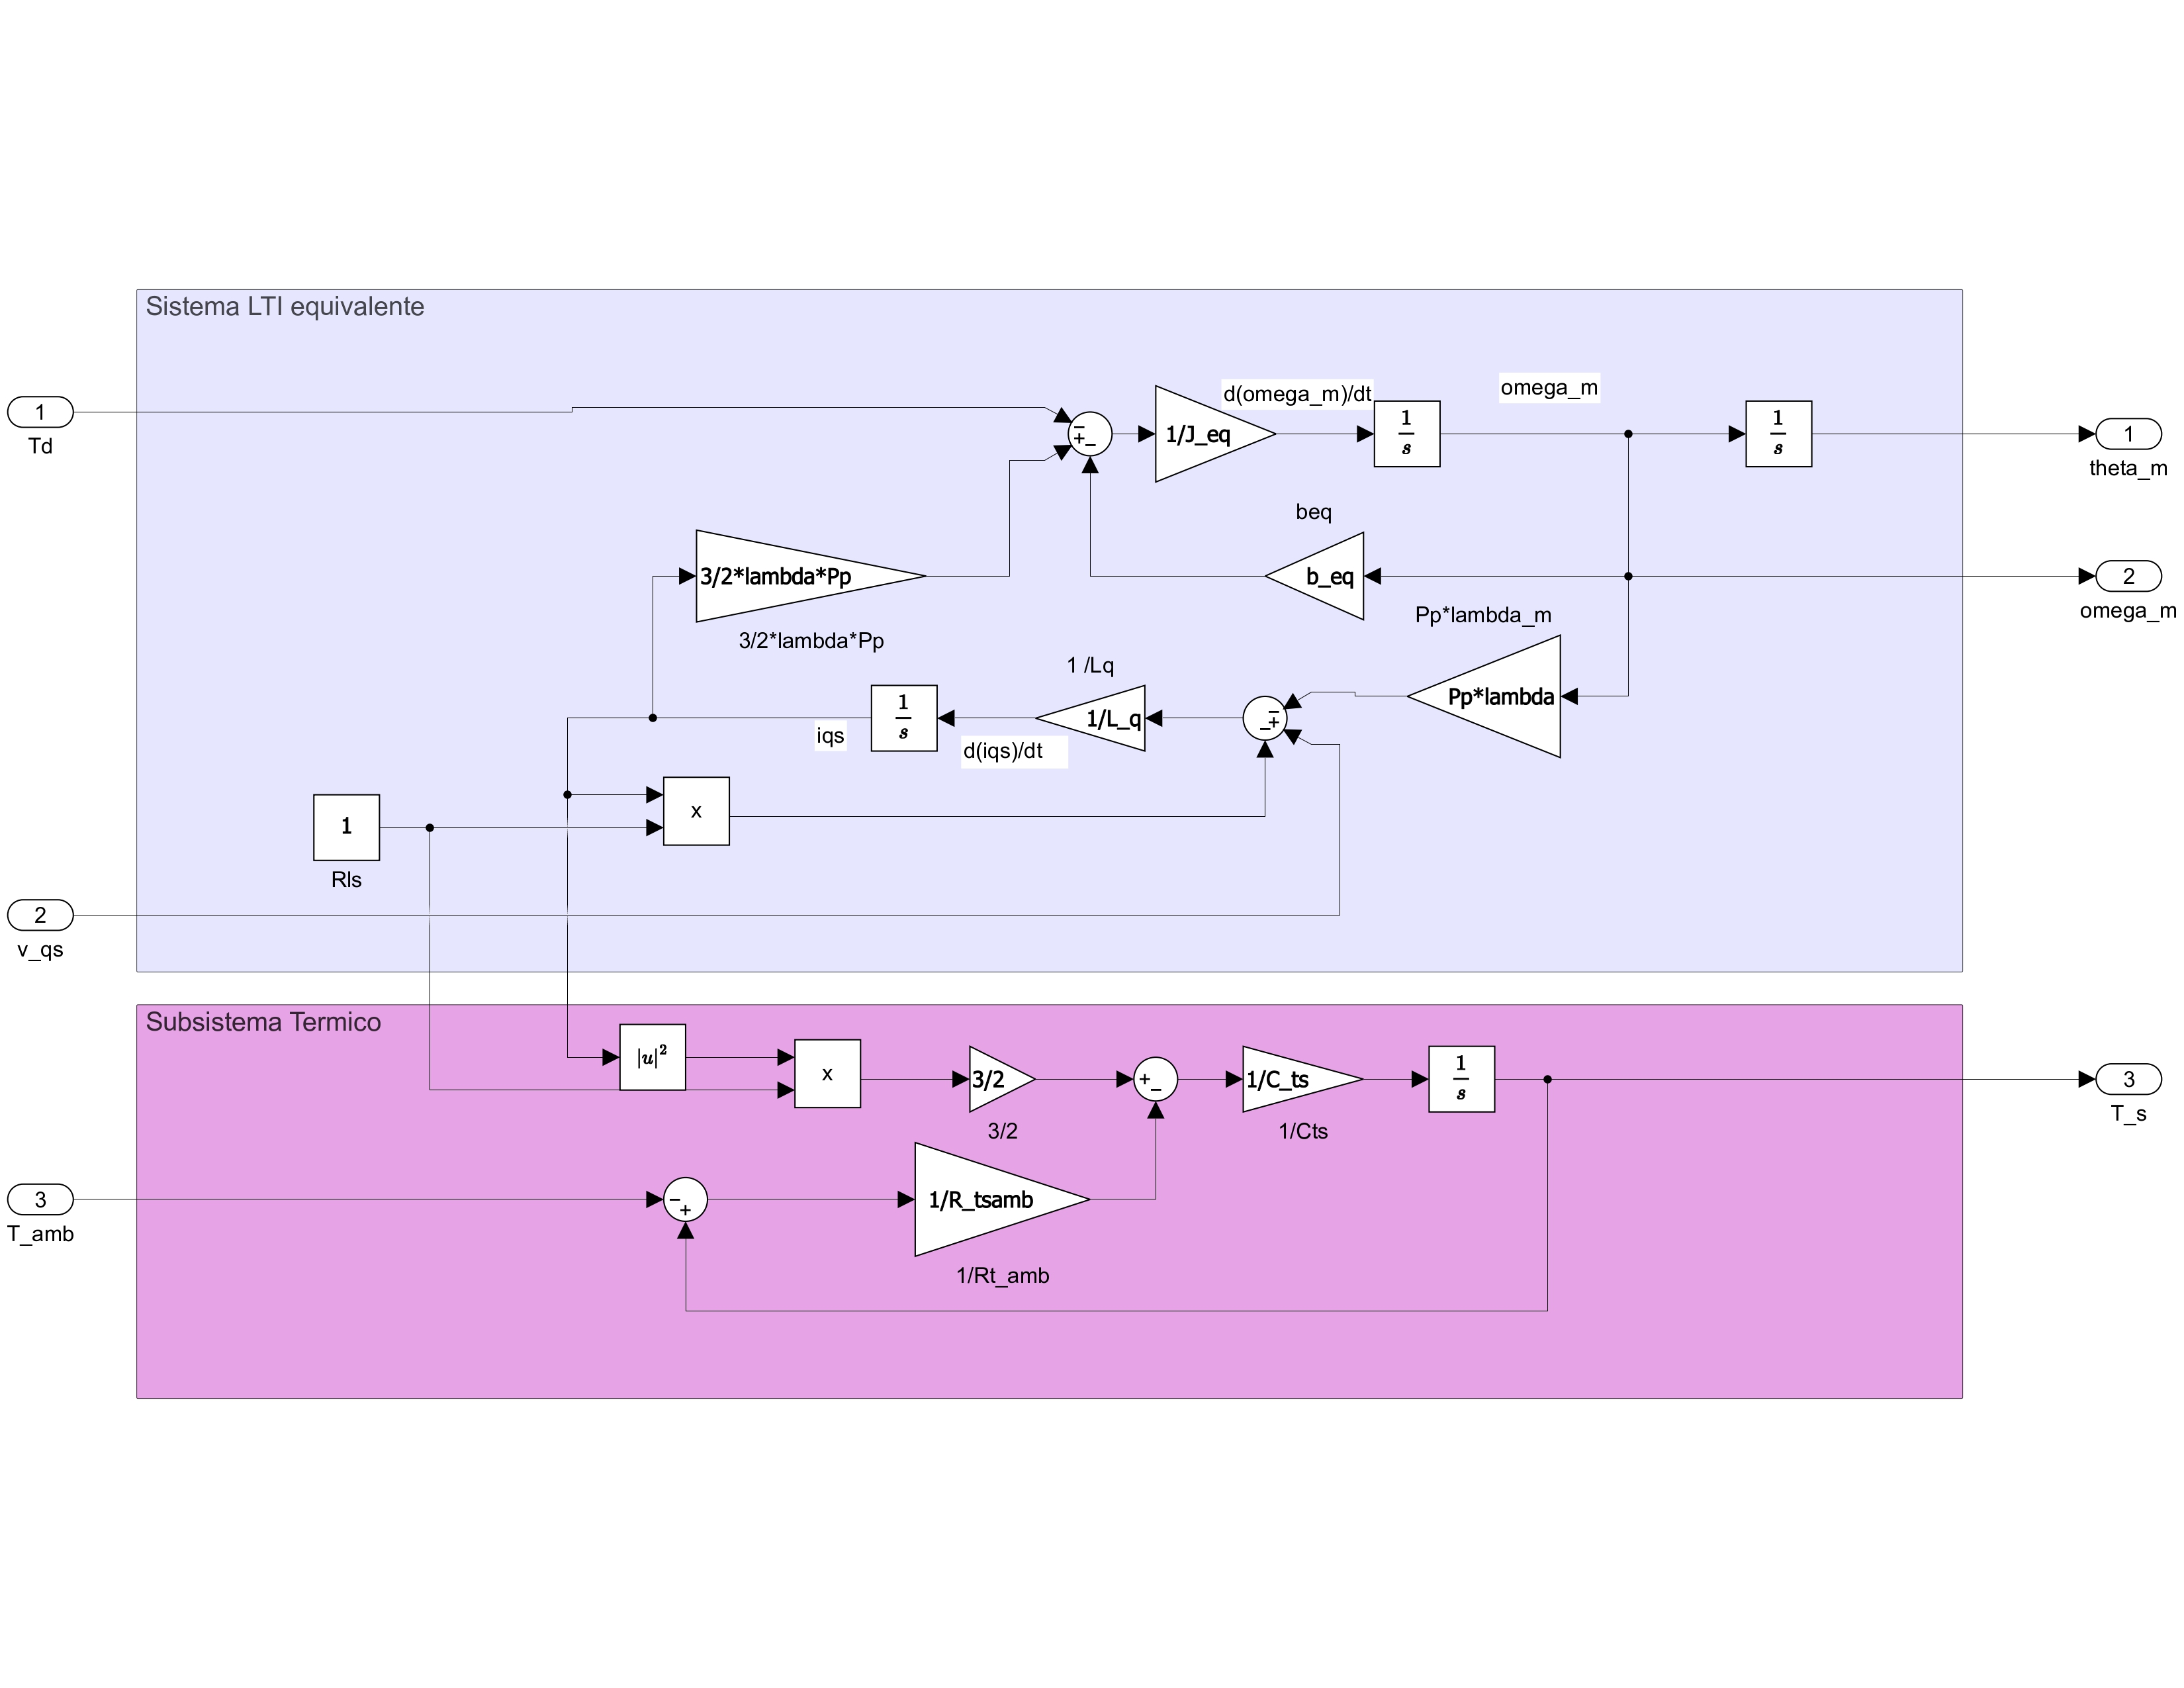
\includegraphics[width=1\linewidth]{attachments/ltiequivalente.jpg}
        \caption{Diagrama de bloques del sistema LTI y subsistema térmico equivalente.}
        \label{fig:ltiequivalente}
    \end{figure}
        

\FloatBarrier
Luego en base al modelo LTI y teniendo en cuenta el caso general en el  que $i^r_{ds}(0)\neq0$ por ende teniendo en cuenta la Ley de Control Mínima complementaria e incorporando la dinámica de la corriente directa se obtiene el sistema LTI aumentado.

\begin{equation}
\begin{aligned}
& \left\{
    \begin{aligned}
        \frac{d\theta_m(t)}{dt} &= \omega_m(t) \\[1.5ex]
        \frac{d\omega_{m}(t)}{dt} &= \frac{1}{J_{eq}} \Bigg[ \frac{3}{2}P_{p} \lambda_{m}^{'r} i_{qs}^{r}(t) - b_{eq}  \omega_{m}(t) - \frac{T_d(t)}{r} \Bigg]  \\[1.5ex]
        \frac{di_{qs}^{r}(t)}{dt}  &= \frac{1}{L_{q} } \left[ v_{qs}^{r}(t) - R_{s}^{\ell} i_{qs}^{r}(t) - \lambda_{m}^{'r}P_{p} \omega_{m}(t) \right] \\[1.5ex]
        \frac{di_{ds}^{r}(t)}{dt} &= -\frac{1}{L_{d}} R_{s}^{\ell} i_{ds}^{r}(t)
    \end{aligned}
\right. \\[2ex]
& \frac{dT_{s}^{\circ}(t)}{dt} = \frac{1}{C_{ts}} \Bigg[ \frac{3}{2} R_{s}^{\ell}\Big(i_{qs}^{2}(t) +i_{ds}^{2}(t)\Big)  - \frac{T_{s}^{\circ}(t) - T_{amb}^{\circ}(t)}{R_{ts-amb}} \Bigg]
\end{aligned}
\end{equation}

Luego expresando de forma matricial de la forma $\dot{x}(t) = Ax(t) + B_u u(t) + B_d d(t)$ queda:
\begin{equation}
\begin{bmatrix}
\frac{d\theta_m(t)}{dt} \\
\frac{d\omega_m(t)}{dt}  \\
\frac{d i^r_{qs}(t)}{dt} \\
\frac{d i^r_{ds}(t)}{dt}
\end{bmatrix}
=\begin{bmatrix}
0 & 1 & 0 & 0 \\
0 & \frac{-b_{eq}}{J_{eq}} & \frac{3}{2}\frac{P_p\lambda_{m} ^{'r}}{J_{eq}} & 0 \\
0 & -\frac{\lambda^{'r}_{m}P_p}{L_q} & -\frac{R^\ell_s}{L_q} & 0 \\
0 & 0 & 0 & -\frac{R_s^\ell}{Ld}
\end{bmatrix}
\begin{bmatrix}
\theta_m(t) \\
\omega_m(t) \\
i_{qs}^r(t) \\
i_{ds}^r(t)
\end{bmatrix}+\begin{bmatrix}
0 \\
0\\
\frac{1}{L_q}\\
0
\end{bmatrix}
v^r_{qs}+\begin{bmatrix}
0 \\
-\frac{1}{J_{eq}r}\\
0 \\
0
\end{bmatrix} 
T_d
\end{equation}

\begin{figure}
    \centering
    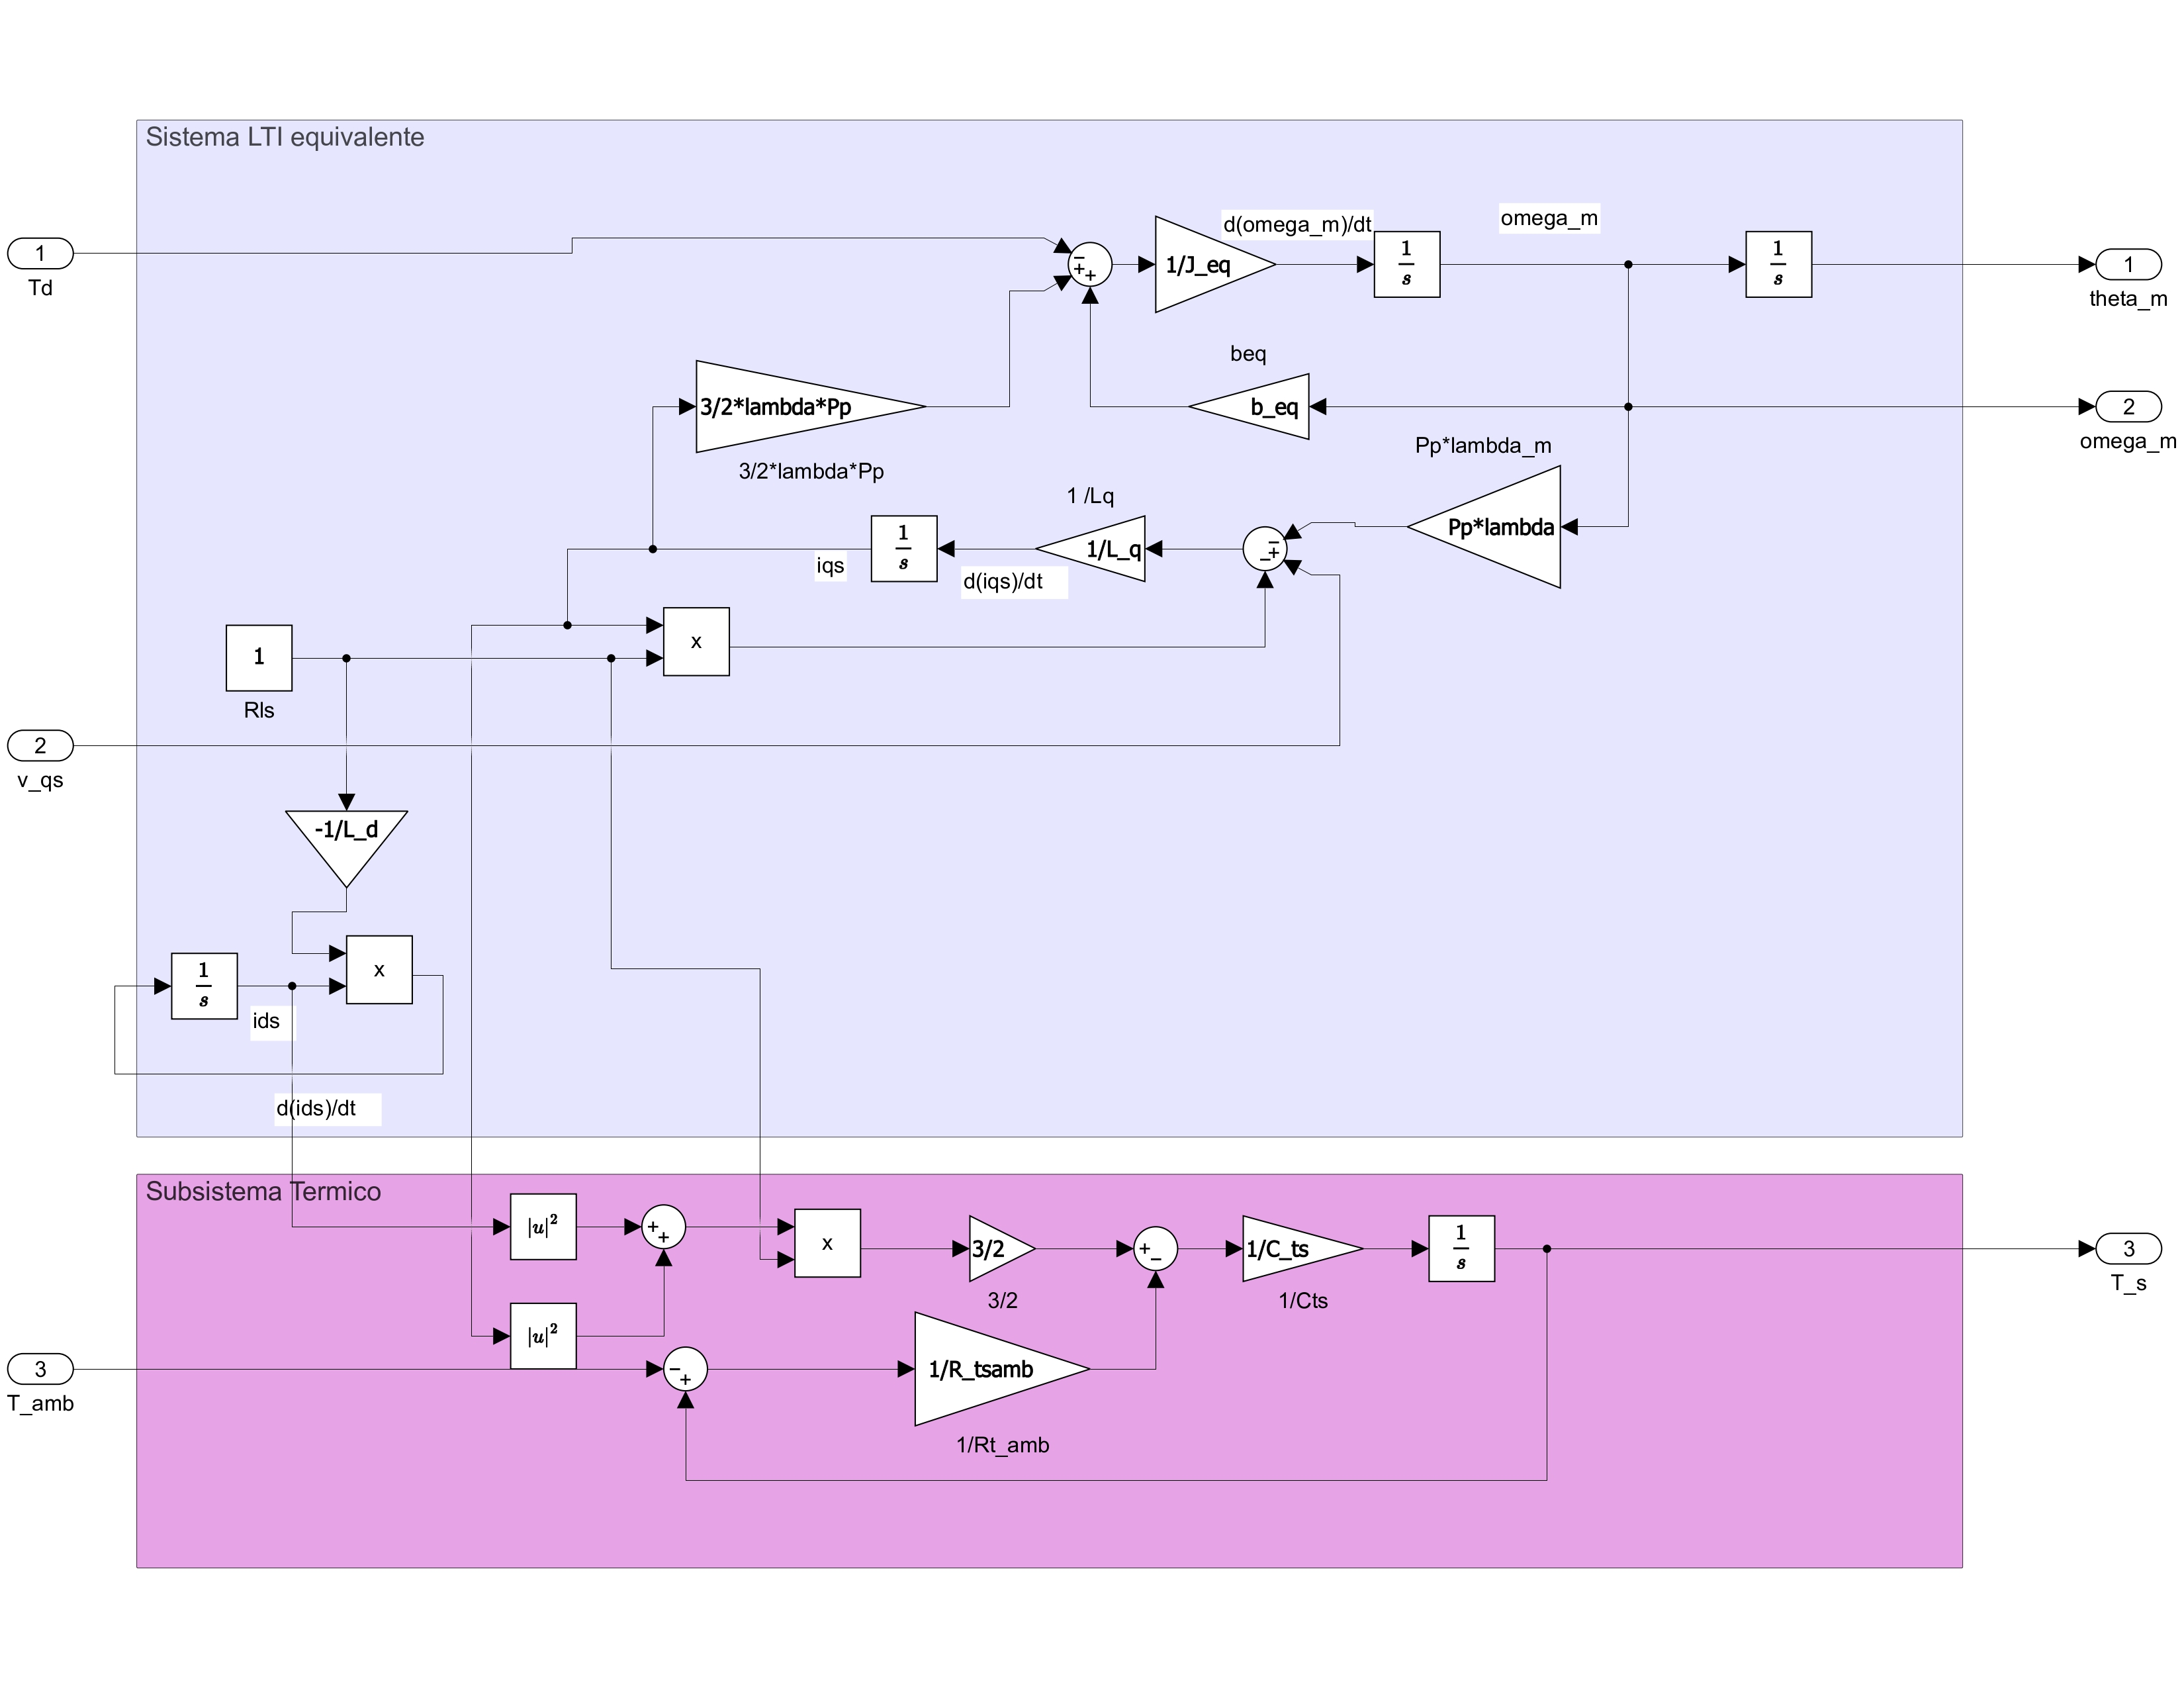
\includegraphics[width=1\linewidth]{attachments/ltiaumentado.jpg}
    \caption{Diagrama de bloques del sistema LTI equivalente aumentado y subsitema térmico equivalente.}
    \label{fig:ltiaumentado}
\end{figure}





\newpage

% ---------------------------------------------------------------------------- %
\subsubsection{Comparación del Modelo Dinámico LTI Equivalente Aumentado vs. el Modelo Dinámico Global LPV}
La evaluación de las estructuras modeladas expone un compromiso directo entre la simplicidad analítica y la precisión representativa. El modelo global LPV abarca el comportamiento general de la planta mediante la inclusión de los fenómenos térmicos sobre $R_s(T_s^\circ(t))$ y los términos de acoplamiento no lineal que vinculan las variables mecánicas y eléctricas. Esta flexibilidad en la formulación flexibiliza la representación matemática del sistema y abre el espectro operacional hacia zonas de trabajo multifuncionales (regímenes de reforzamiento y debilitamiento de campo).  En sentido inverso, la implementación del modelo LTI equivalente aumentado recurre a la restricción operativa de imponer $i^r_{ds} \equiv 0$, extinguiendo la influencia de la corriente directa sobre la dinámica electromecánica global. Si bien este procedimiento linealiza e independiza los canales de control (simplificando la estructura matricial de estado del sistema), reduce el rango operativo local a las proximidades de la condición cuasi-estacionaria de diseño. Consecuentemente, el modelo LTI disminuye su fidelidad ante variaciones dinámicas rápidas fuera de dicho entorno, pero ratifica su aptitud analítica para predecir con solvencia el estado estacionario y las tendencias macroscópicas del sistema bajo estudio. 

\subsubsection{Efectos de la Corriente de Eje Directo: Debilitamiento y Reforzamiento de Campo}
Se evaluará el comportamiento del modelo LPV para otros puntos de operación tales como: -$i_{ds}^r>0$ (reforzamiento de campo) -$i_{ds}^r<0$ (debilitamiento del campo). Al analizar el sistema se concluye que estos cambios se ven reflejados principalmente en las siguientes ecuaciones: -la ecuación del torque electromagnetico \ref{SubElec3}   y -la ecuación de la variación de la corriente del eje en cuadratura \ref{variacion_ids} 
$$ T_{m}(t)   = \frac{3}{2}P_{p} \lambda_{m}^{'r} i_{qs}^{r}(t) + \frac{3}{2} P_{p} \Big( L_{d} - L_{q} \Big) i_{qs}^{r}(t) i_{ds}^{r}(t)$$
$$ \frac{di_{ds}^{r}(t)}{dt}  = \frac{1}{L_{d}} \left[ v_{ds}^{r}(t) - R_{s} \Big( T_{s}^{\circ} (t) \Big) i_{ds}^{r}(t) + L_{q}i_{qs}^{r}(t) \omega_{m}(t)P_{p}  \right] $$
Luego considerando un estado estacionario $(\frac{di_{ds}^r}{dt}=0)$ es posible despejar la velocidad angular del motor $\omega_m=$, quedando:
\begin{equation}    
\omega_{m}(t) = \frac{R_{s} \Big( T_{s}^{\circ} (t) \Big) i_{ds}^{r}(t) - v_{ds}^{r}(t)}{P_{p} L_{q} i_{qs}^{r}(t)}
\end{equation}

Analizando la ecuación de torque electromagnético y la ecuación de velocidad angular del motor para cada caso (teniendo en cuenta que es una máquina de polos salientes donde $L_d>L_q$:
\begin{itemize}
    \item Caso $i^r_{ds0}>0$ (Reforzamiento de campo):
    
    Dado que $L_d > L_q$, el término de reluctancia $(L_d - L_q)i_{ds}^r$ incrementa el flujo magnético efectivo en la ecuación del torque. Como consecuencia, el par motor disponible $T_m$ se refuerza (aumenta) a bajas velocidades. En contraparte, al evaluar la velocidad angular en régimen estacionario, los términos en el numerador de su expresión matemática se oponen, provocando que la velocidad de equilibrio disminuya bajo una potencia aproximadamente constante.
    \[
    i_{ds0}^{r} > 0 \implies \left\{ 
    \begin{aligned}
    T_{m} &\uparrow \quad \text{(se refuerza)} \\
    \omega_{m} &\downarrow \quad \text{(se reduce)}
    \end{aligned}
    \right.
    \]

    \item Caso $i^r_{ds0}<0$ (Debilitamiento de campo):
    
    En este escenario, el término $(L_d - L_q)i_{ds}^r$ se vuelve negativo, reduciendo el flujo efectivo, lo que se traduce en una disminución del torque electromagnético desarrollado $T_m$. Por otra parte, analizando la velocidad angular de rotación, el término óhmico $R_s i_{ds}^r$ en el numerador adopta un signo negativo que se acopla con la tensión de control. Esto reduce la contratensión requerida, permitiendo un incremento significativo de la velocidad de equilibrio de la máquina sin sobrepasar el límite de tensión impuesto por el inversor.   
    \[
    i_{ds0}^{r} < 0 \implies \left\{ 
    \begin{aligned}
    T_{m} &\downarrow \quad \text{(se reduce)} \\
    \omega_{m} &\uparrow \quad \text{(se refuerza)}
    \end{aligned}
    \right.
    \]
\end{itemize}





\subsubsection{Funciones de Transferencia}
Analizando las ecuaciones del sistema LTI equivalente aumentado que implican a las entradas $v^r_{qs}$ y $T_l$ hacia la salida $\theta_m$. Los cuaales son:
\begin{equation}
\left\{
\begin{aligned}
\frac{d\theta_m(t)}{dt} &= \omega_m(t) \\[1.5ex]
\frac{d\omega_{m}(t)}{dt} &= \frac{1}{J_{eq}} \Bigg[ \frac{3}{2}P_{p} \lambda_{m}^{'r} i_{qs}^{r}(t) - b_{eq} \omega_{m}(t) - \frac{T_d(t)}{r} \Bigg]  \\[1.5ex]
\frac{di_{qs}^{r}(t)}{dt}  &= \frac{1}{L_{q} } \left[ v_{qs}^{r}(t) - R_{s}^{\ell} i_{qs}^{r}(t) - \lambda_{m}^{'r}P_{p} \omega_{m}(t) \right]
\end{aligned}
\right.
\end{equation}
A estas les aplicamos la transformada de Laplace considerando las condiciones iniciales nulas


\begin{equation}
\left\{
\begin{aligned}
s\Theta_m(s) &= \Omega_m(s)\\
s\Omega(s) &= \frac{1}{J_{eq}}\Big(\frac{3}{2}P_p\lambda^{'r}_mI^r_{qs}(s)-b_{eq}\Omega_m(s)-\frac{T_d(s)}{r}\Big)\\
sI^r_{qs}(s) &= \frac{1}{L_q}\Big(V^r_{qs}(s)-R^\ell_{s}I^r_{qs}(s)-\lambda^{'r}_mP_p\Omega_m(s)\Big)
\end{aligned}
\right.
\end{equation}
Trabajando matemáticamente llegamos a la siguiente igualdad:
\begin{equation}
    \Theta_m(s) = \frac{3P_p\lambda_m^{'r}V_{qs}^r(s)-2\Big(L_qs+R^\ell_s\Big)\frac{T_d(s)}{r}}{2J_{eq}L_qs^3+2\Big(J_{eq}R_s^\ell+b_{eq}L_q\Big)s^2+\Big(2b_{eq}R_s^\ell+3\Big(P_p\lambda^{'r}_m\Big)^2\Big)s}
\end{equation}
Por lo tanto, las funciones de transferencia para las entradas $V^r_{qs}(s)$ y $T_d(s)$:
\begin{equation}
    G_{V^r_{qs}}(s)=\frac{\Theta_m(s)}{V_{qs}^r(s)} = \frac{3P_p\lambda_m^{'r}}{2J_{eq}L_qs^3+2\Big(J_{eq}R_s^\ell+b_{eq}L_q\Big)s^2+\Big(2b_{eq}R_s^\ell+3\Big(P_p\lambda^{'r}_m\Big)^2\Big)s}    
\end{equation}
\begin{equation}
    G_{T_d}(s)=\frac{\Theta_m(s)}{T_d(s)}= \frac{-2\Big(L_qs+R^\ell_s\Big)\frac{1}{r}}{2J_{eq}L_qs^3+2\Big(J_{eq}R_s^\ell+b_{eq}L_q\Big)s^2+\Big(2b_{eq}R_s^\ell+3\Big(P_p\lambda^{'r}_m\Big)^2\Big)s}
\end{equation}
Ed ésta manera podemos expresar al sistema tal que: 
\begin{equation}
    \Theta_m(s)=G_{V^r_{qs}}(s)V^r_{qs}(s)+G_{T_d}(s)T_d(s)
\end{equation}
% ---------------------------------------------------------------------------- %
\subsection{Análisis de Estabilidad a lazo abierto para el modelo LTI equivalente aumentado}
Para analizar la estabilidad se utiliza evalúan los polos y ceros del sistema. Al evaluar el polinomio característico se obtienen los polos del sistema, el polinomio característico es el denominador de las funciones de transferencia:
\begin{equation}
    2J_{eq}L_qs^3+2\Big(J_{eq}R_s^\ell+b_{eq}L_q\Big)s^2+\Big(2b_{eq}R_s^\ell+3\Big(P_p\lambda^{'r}_m\Big)^2\Big)s
\end{equation}
Para obtener los polos del sistema LTI equivalente aumentado se iguala el polinomio característico a cero y se evalúan las raíces del polinomio:
\begin{equation}
    2J_{eq}L_qs^3+2\Big(J_{eq}R_s^\ell+b_{eq}L_q\Big)s^2+\Big(2b_{eq}R_s^\ell+3\Big(P_p\lambda^{'r}_m\Big)^2\Big)s=0
\end{equation}
como podemos aplicar factor común de $s$ se concluye que uno de los polos se encuantra en $s_1=0$, por consiguiente evaluando lo que queda luego del factor común (una ecuación de segundo grado). Así los polos son los siguientes: 

\begin{equation}
    \begin{cases} 
        s_1 = 0 \\ 
        s_{2,3} = \frac{-2\left(J_{eq}R_s^\ell+b_{eq}L_q\right) \pm \sqrt{4\left(J_{eq}R_s^\ell+b_{eq}L_q\right)^2 - 8J_{eq}L_q\left(2b_{eq}R_s^\ell+3\left(P_p\lambda^{'r}_m\right)^2\right)}}{4J_{eq}L_q} 
    \end{cases}
\end{equation}
Ahora para obtener los cero se evalúan los numeradores de las funciones de transferencia. Al analizar los numeradores se denota que al igualar a cero los numeradores lo único que queda es la siguiente expresión 
\begin{equation}
    L_qs+R^\ell_s=0
\end{equation}
Al despejar llegamos al cero del sistema 
\begin{equation}
    s=-\frac{R^\ell_s}{L_q}
\end{equation}
Luego reemplazando los valores de las variables y variando el valor de temperatura lo que varia $R_s^\ell$
\begin{table}[htbp]
\centering
\caption{Resistencia, Polos y Ceros del sistema variando la Temperatura con $J_{eq}=19,78*10^{-6}$ (mínimo).}
\label{tab:polosyceros}
\begin{tabular}{lllll}
\hline
$T^\circ_s(\circ C) $&$ R^\ell_s $&$ p_1 $&$ p_2 $&$ z $\\
\hline
 $ 20$&$1,0200 $  & $-88,49+149,97 i$     & $  -88,49-149,97 i$    &$ -175.8621 $ \\
 $ 40$&$ 1,0996  $ &$ -95,34+145,75 i$     & $-95,34- 145,75 i$     & $-189.5793  $\\
  $60$&$ 1,1791$  & $-102,20+141,08 i $    &$-102,20-141,08 i $     &$-203.2966 $\\
  $  80$&$1,2587$   &$ -109,06+135,91 i $    &$-109,06-135,91 i $     & $-217.0138  $\\
    $100$& $1,3382$  & $-115,92+130,17 i $    &$-115,92-130,17 i$      &$ -230.7310$  \\
   $ 120$&$ 1,4178$  &$ -122,78+123,78 i$     &$-122,78-123,78 i$      & $-244.4483  $\\
   $ 140$&$ 1,4974  $&$-129,64+116,64 i $     &$-129,64-116,64 i $     &$ -258.1655  $\\
\hline
\end{tabular}
\end{table}
\begin{figure}[h]
    \centering
    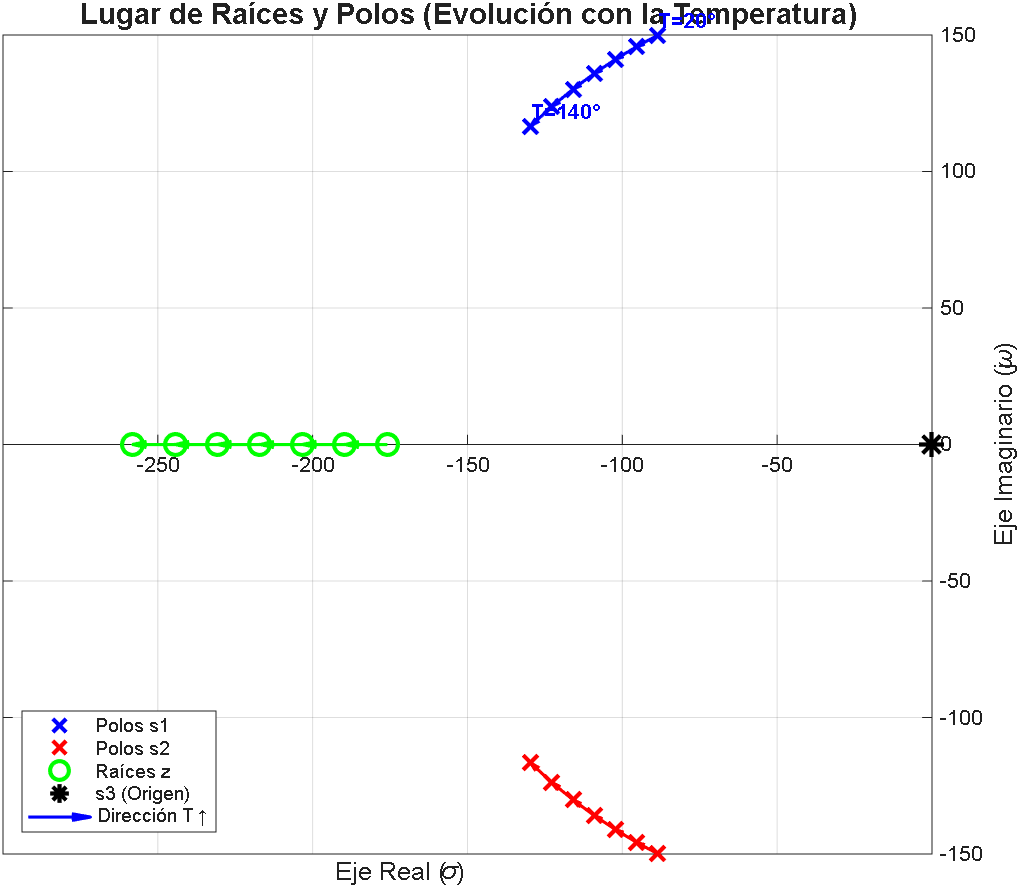
\includegraphics[width=0.75\linewidth]{attachments/polosyceros.png}
    \caption{Polos y Ceros del sistema variando la Temperatura con $J_{eq}=19,78*10^{-6}$ (mínimo)}
    \label{fig:placeholder}
\end{figure}
A realizar el análisis se aprecia que tanto los polos como los ceros del sistema se encuentran en el semiplano con parte real negativa del plano complejo, con esto concluímos que el sistema es estable. Tmabién podemos ver que al aumentar la temperatura que implica aumento de la resistencia los polos se mantiene en el mismo semiplano del plano complejo, por lo que incluso al variar $R^\ell_s$ dentro del rango el sistema se mantiene estable. 

% ---------------------------------------------------------------------------- %
\subsection{Análisis de Observabilidad completa de estado para el modelo LTI equivalente aumentado}
Para evaluar la observabilidad completa de estado del modelo LTI equivalente aumentado (considerando la ley de control mínima $i_{ds}^{r}(t) \equiv 0$  y despreciando el efecto de la temperatura $T_{s}^{o}(t)$) desde la variable de salida $\theta_m(t)$, se emplea el criterio de Kalman. Este criterio establece que un sistema LTI de orden $n$ es completamente observable si el rango de la matriz de observabilidad $\mathcal{O}$ es igual a $n$. En consecuencia, dado que $\mathcal{O}$ es una matriz cuadrada, el sistema será observable si su determinante es distinto de cero ($\det(\mathcal{O}) \neq 0$).

La matriz de observabilidad $\mathcal{O}$ queda definida tal que:
\begin{equation}
\mathcal{O} = \begin{bmatrix}
C \\
CA \\
CA^2 \\
\vdots \\
CA^{n-1}
\end{bmatrix}
\end{equation}
Donde: 
$
A = \begin{bmatrix}
0 & 1 & 0 \\
0 & \frac{-b_{eq}}{J_{eq}} & \frac{3}{2}\frac{P_p\lambda_{m}^{'r}}{J_{eq}} \\
0 & -\frac{\lambda^{'r}_{m}P_p}{L_q} & -\frac{R^\ell_s}{L_q}
\end{bmatrix}
$;
$C=\begin{bmatrix}
    1& 0& 0
\end{bmatrix}$ (considerando como salida la posición
angular del motor $\theta_m$) 

Entonces la matriz de observabilidad queda: 
\begin{equation}
    \mathcal{O}_{\theta_m} = \begin{bmatrix}
C \\
CA \\
CA^2
\end{bmatrix}=\begin{bmatrix}
1 & 0 & 0 \\
0 & 1 & 0 \\
0 & -\frac{b_{eq}}{J_{eq}} & \frac{3}{2}\frac{P_p\lambda_{m}^{'r}}{J_{eq}}
\end{bmatrix}
\end{equation}
Luego al evaluar el determinante de la matriz de observabilidad se obtiene: $det(\mathcal{O}_{\theta_m})=\frac{3}{2}\frac{P_p\lambda_{m}^{'r}}{J_{eq}}$, como se sabe que $\frac{3}{2}\frac{P_p\lambda_{m}^{'r}}{J_{eq}} \neq 0$ por ende se concluye que el sistema es totalmente observable desde $\theta_m$.

Si ahora se evalúa la observabilidad de la salida $\omega_m$, donde $C$ para a ser $C=\begin{bmatrix}
    0&1&0
\end{bmatrix}$


\begin{equation}
    \mathcal{O}_{\omega_m} = \begin{bmatrix}
0 & 1 & 0 \\
0 & -\frac{b_{eq}}{J_{eq}} & \frac{3}{2}\frac{P_p\lambda_{m}^{'r}}{J_{eq}} \\
0 & \left( \frac{b_{eq}^2}{J_{eq}^2} - \frac{3}{2}\frac{P_p^2 (\lambda_{m}^{'r})^2}{J_{eq}L_q} \right) & -\frac{3}{2}\frac{P_p\lambda_{m}^{'r}}{J_{eq}} \left( \frac{b_{eq}}{J_{eq}} + \frac{R^\ell_s}{L_q} \right)
\end{bmatrix}
\end{equation}
evaluando el determinante 


$det(\mathcal{O_{\omega_m}})=0$ a través de este análisis se ve que que no el sistema no es totalmente observable desde $\omega_m$. Por consecuencia es correcto decir que la alternativa de medición con tacogenerador no es viable si se desea realizar un control de posición de alta precisión, debido a que un observador de estado nunca podría reconstruir la posición real de la carga en base únicamente en la señal del tacogenerador.

% ---------------------------------------------------------------------------- %
\subsection{Análisis de Controlabilidad completa de estado para el modelo LTI equivalente aumentado }
Nuevamente con el criterio de Kalman se analizará la controlabilidad completa del sistema LTI equivalente aumentado (considerando la ley de control mínima $i_{ds}^{r}(t) \equiv 0$  y despreciando el efecto de la temperatura $T_{s}^{o}(t)$) desde la entrada manipulada $v_{qs}^r(t)$ sin considerar la perturbación de la carga mecánica, es decir, teniendo en cuanta solo $B$ sin $B_w$ para calcular la matriz de controlabilidad del sistema:
\begin{equation}
    C = \begin{bmatrix} B & AB & \cdots & A^{n-1}B \end{bmatrix}
\end{equation}
Donde: $
A = \begin{bmatrix}
0 & 1 & 0 \\
0 & \frac{-b_{eq}}{J_{eq}} & \frac{3}{2}\frac{P_p\lambda_{m}^{'r}}{J_{eq}} \\
0 & -\frac{\lambda^{'r}_{m}P_p}{L_q} & -\frac{R^\ell_s}{L_q}
\end{bmatrix}
$;$\begin{bmatrix}
0 \\
 0\\
 \frac{1}{L_q}
\end{bmatrix}$
Con esto la matriz de Controlabilidad es la siguiente: 
\begin{equation}
C = \begin{bmatrix} B & AB & A^2B \end{bmatrix} = \begin{bmatrix}
0 & 0 & \frac{3}{2}\frac{P_p \lambda_{m}^{'r}}{J_{eq} L_{q}} \\
0 & \frac{3}{2}\frac{P_p \lambda_{m}^{'r}}{J_{eq} L_{q}} & -\frac{3}{2}\frac{P_p \lambda_{m}^{'r} b_{eq}}{J_{eq}^2 L_{q}} - \frac{3}{2}\frac{P_p R^\ell_s \lambda_{m}^{'r}}{J_{eq} L_{q}^2} \\
\frac{1}{L_{q}} & -\frac{R^\ell_s}{L_{q}^2} & \frac{(R^\ell_s)^{2}}{L_{q}^3} - \frac{3}{2}\frac{P_p^{2} (\lambda_{m}^{'r})^{2}}{J_{eq} L_{q}^2}\end{bmatrix}
\end{equation}

Y su determinante: $det(C)=-\frac{9}{4} \frac{P_p^2 (\lambda_{m}^{'r})^2}{J_{eq}^2 L_q^3}\neq 0$, con el cuál se concluye debido a que $det(C) \neq 0$ se concluye que el sistema es completamente controlable desde la variable manipulada $v_{qs}(t)$


% ---------------------------------------------------------------------------- %
\subsection{Simulación Dinámica en el Dominio del Tiempo, comparando el Modelo NL Completo Desacoplado con Ley de Control NL vs LTI Equivalente Aumentado}
Se analizara la respuesta del estado interno \{$\theta_m(t);\omega_m(t);i_{dq0s}(t);T^\circ_s(t)$\} ante consignas de tensión de amplitud ${v^r_{qs}}^*$ superpuesta con una perturbación $T_l$. Siendo las entradas las siguientes:
\begin{figure}[h]
    \centering
    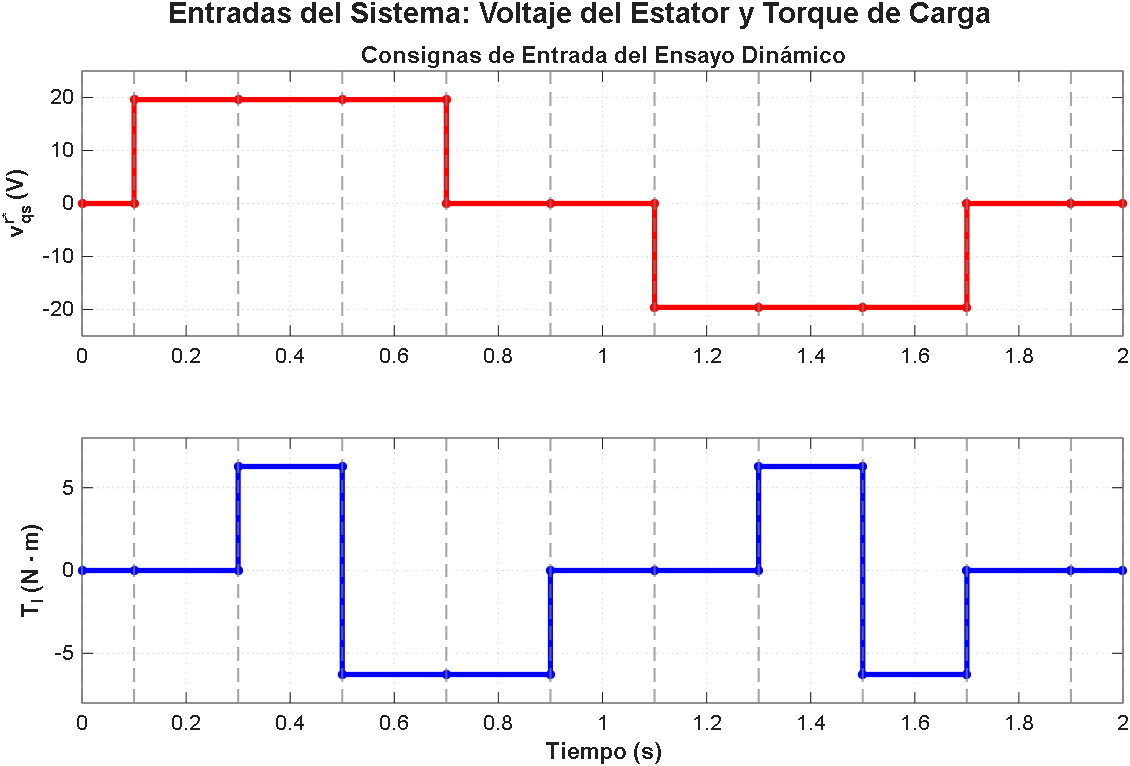
\includegraphics[width=0.6\linewidth]{attachments/VariacionTorqueyTension.png}
    \caption{Entrada de tensión y de torque de perturbación para simulación dinámica.}
    \label{fig:placeholder}
\end{figure}

\FloatBarrier
Considerando la $T_{amb}=20^\circ C$ 

\begin{figure}[h]
    \centering
    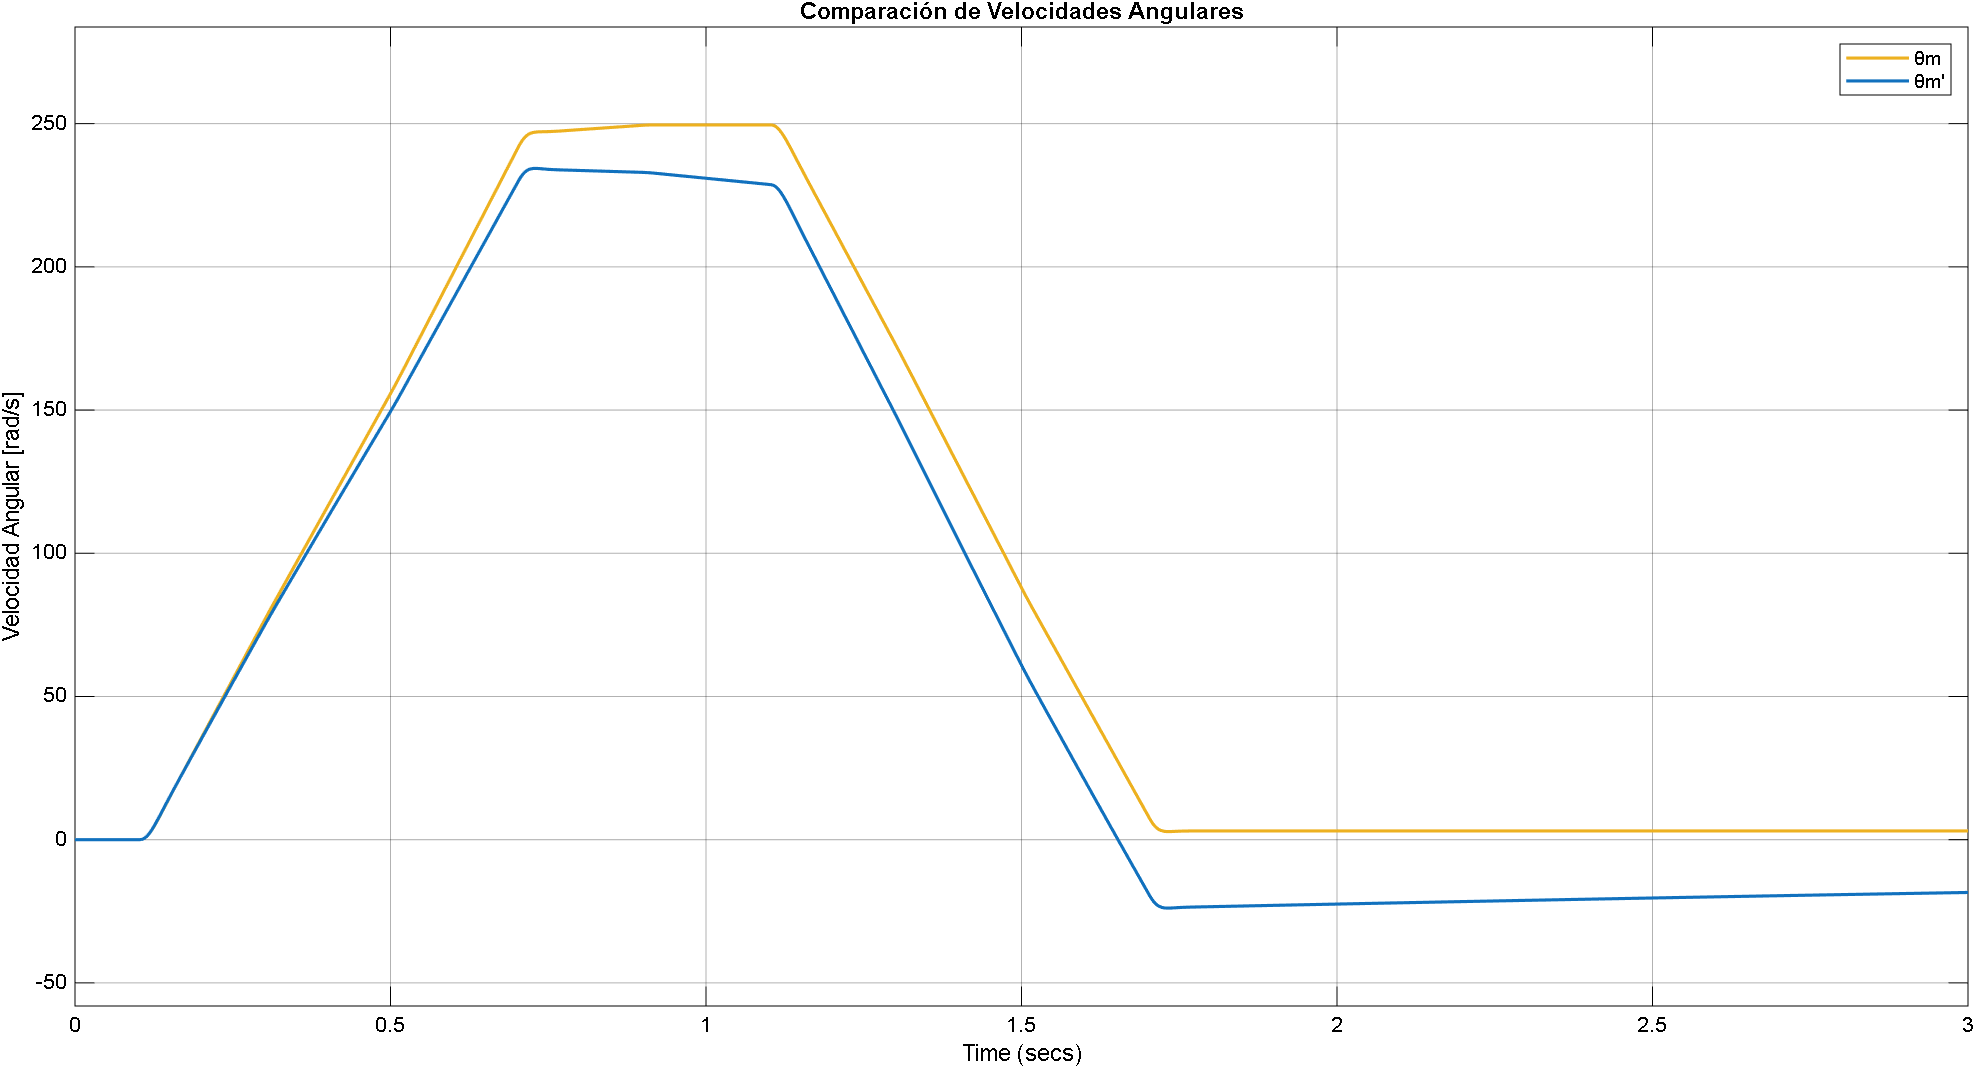
\includegraphics[width=0.6\linewidth]{attachments/Compa_NL_LTI_posici_ang.png}
    \caption{Posición Angular respecto a Tiempo}
    \label{fig:placeholder}
\end{figure}

\FloatBarrier
\begin{figure}[h]
    \centering
    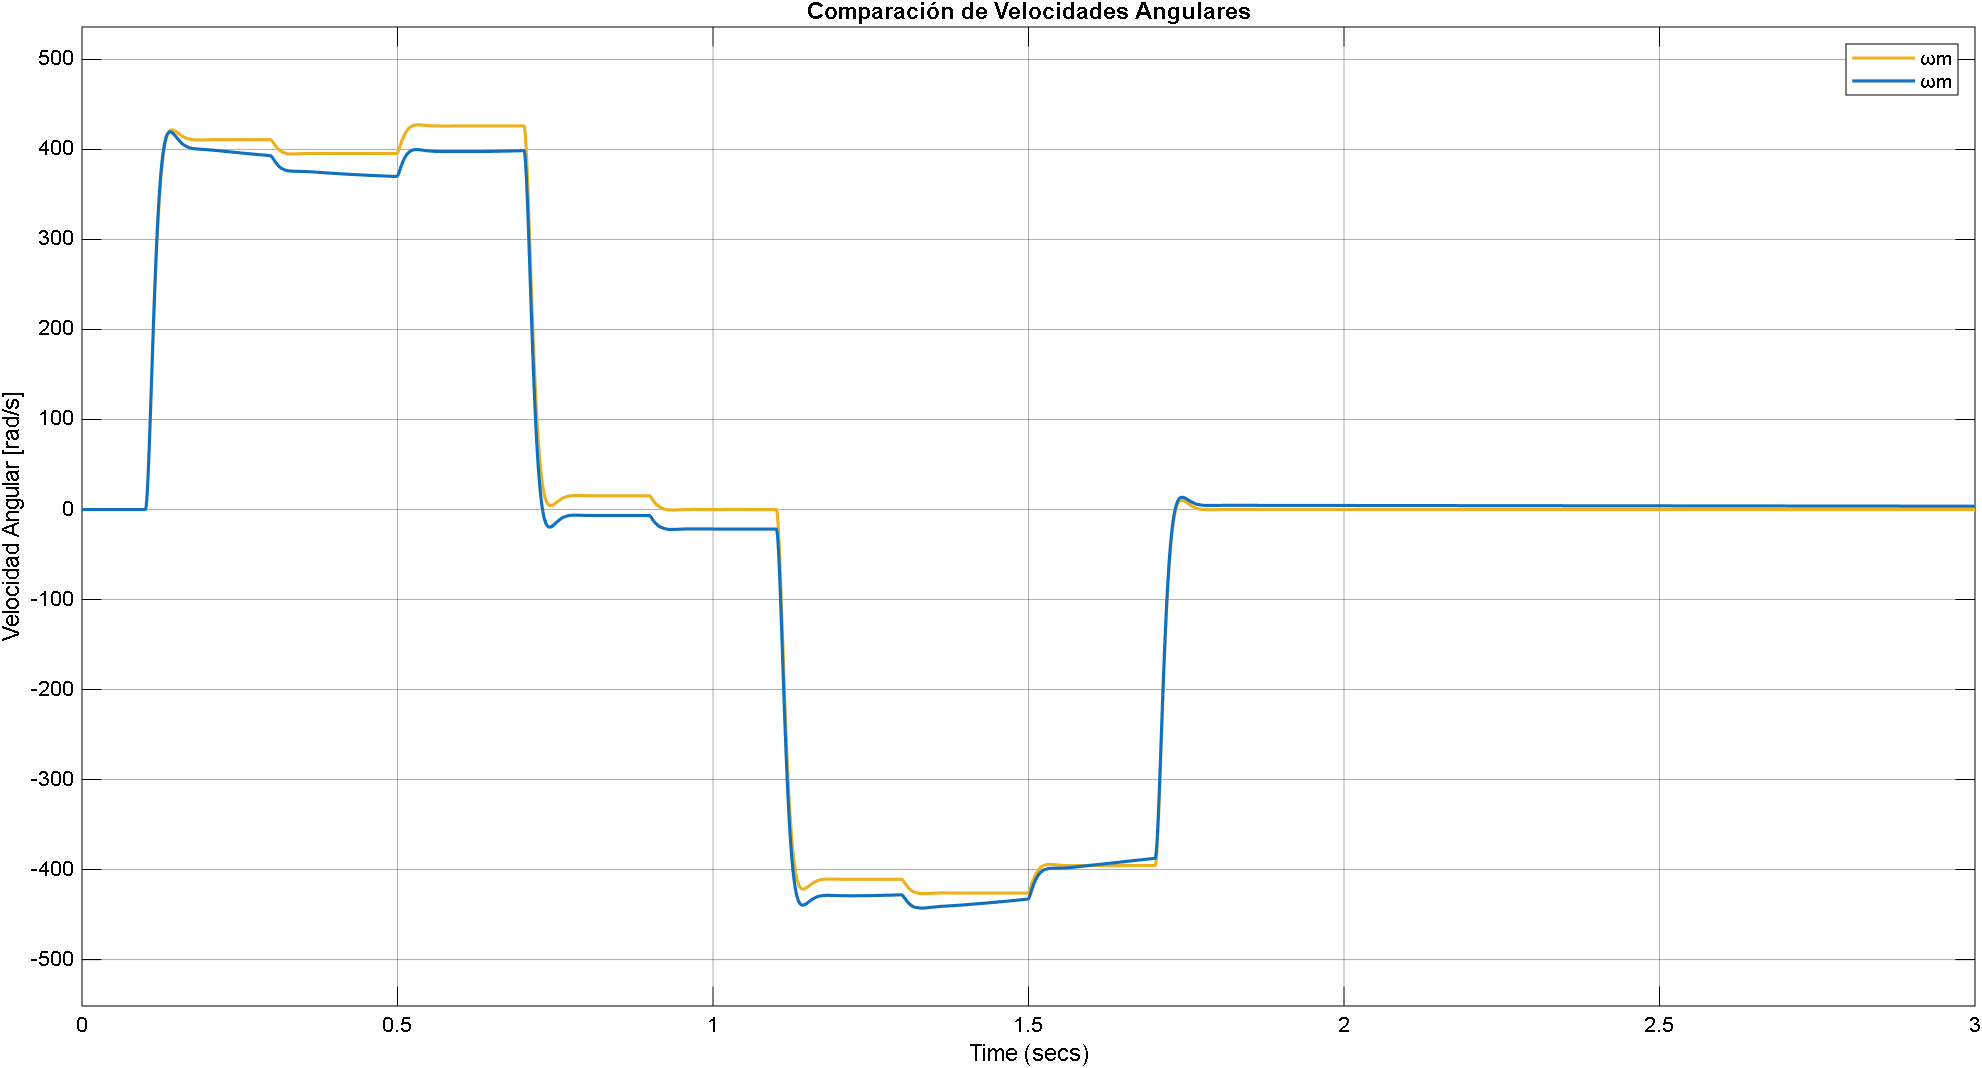
\includegraphics[width=0.6\linewidth]{attachments/Compa_NL_LTI_vel_ang.png}
    \caption{Velocidad Angular respecto al Tiempo}
    \label{fig:placeholder}
\end{figure}

\FloatBarrier
\begin{figure}[h]
    \centering
    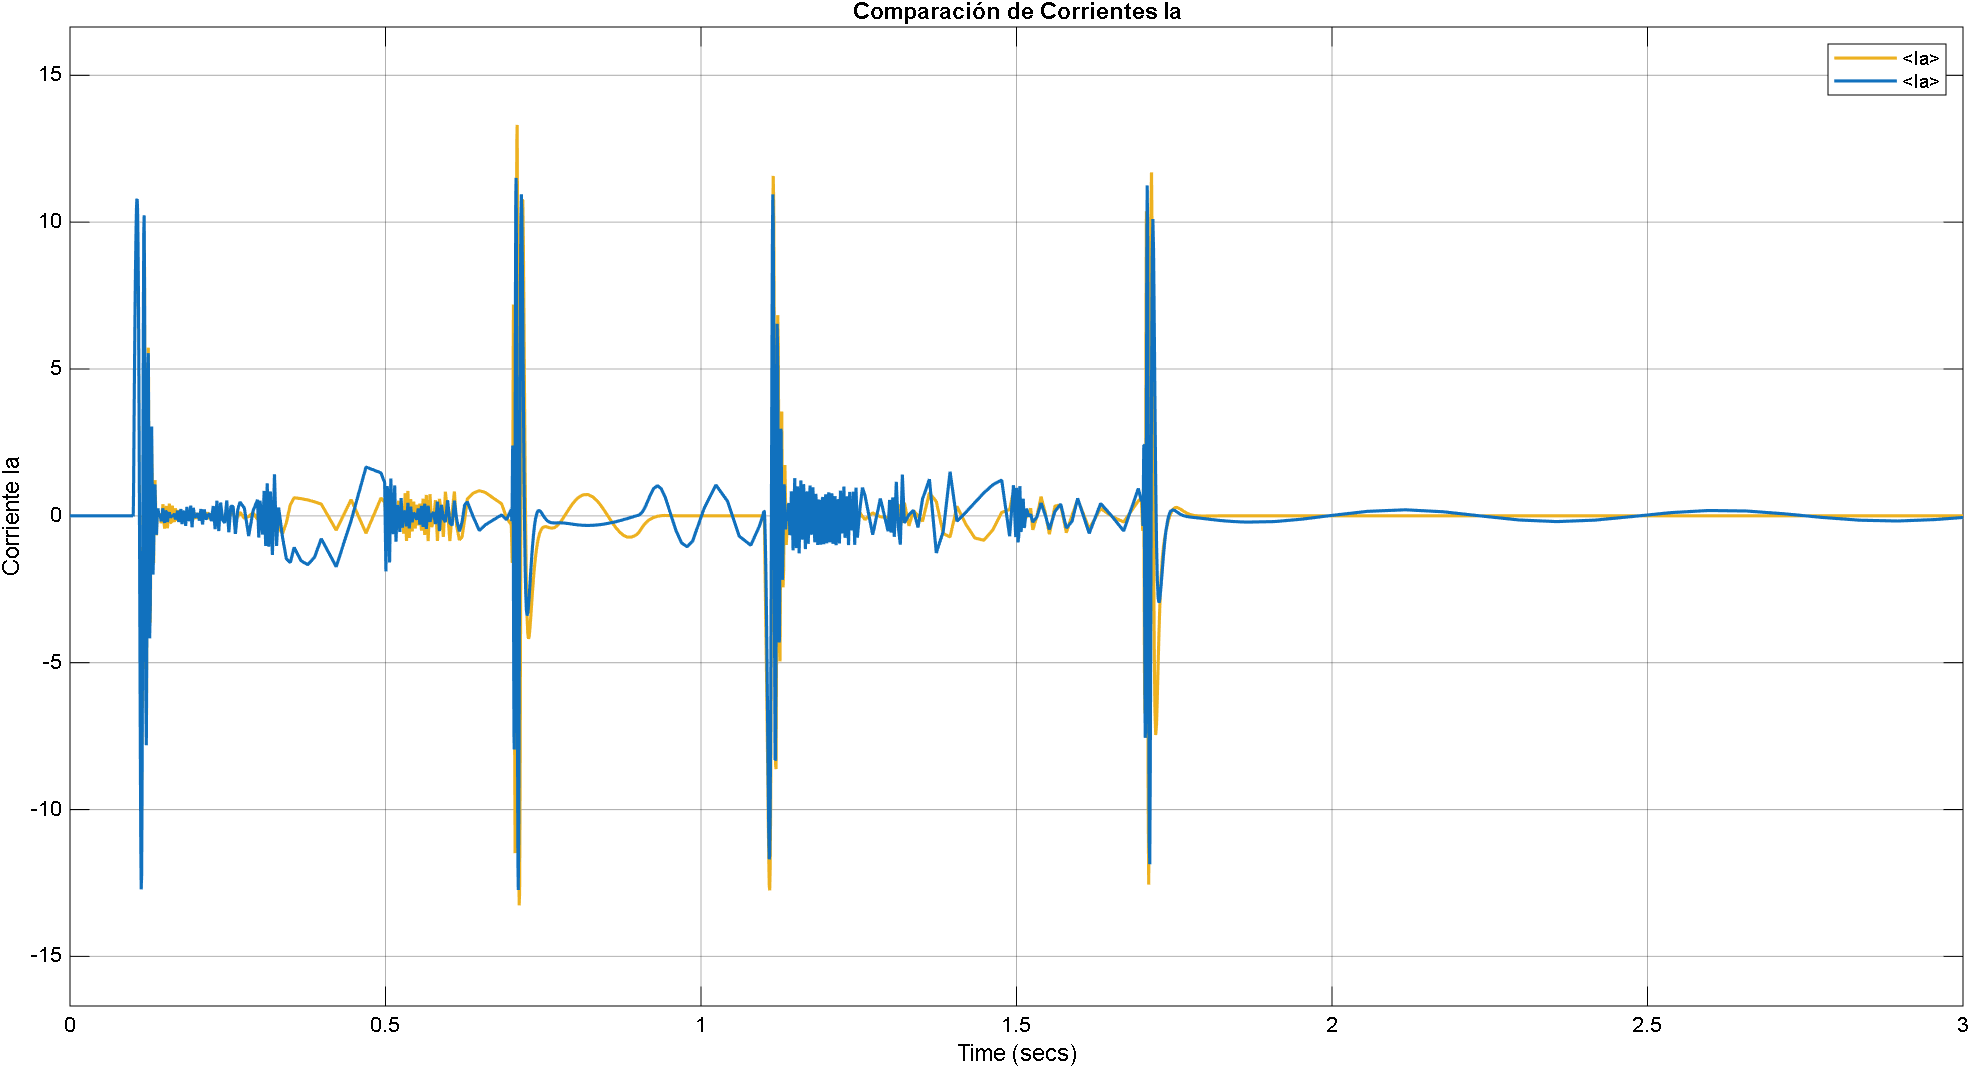
\includegraphics[width=0.6\linewidth]{attachments/Compa_NL_LTI_Ia.png}
    \caption{Corriente Ia respecto al Tiempo (Amarillo->LTI Aumentado; Azul-> NL con Ley}
    \label{fig:placeholder}
\end{figure}

\FloatBarrier
\begin{figure}[h]
    \centering
    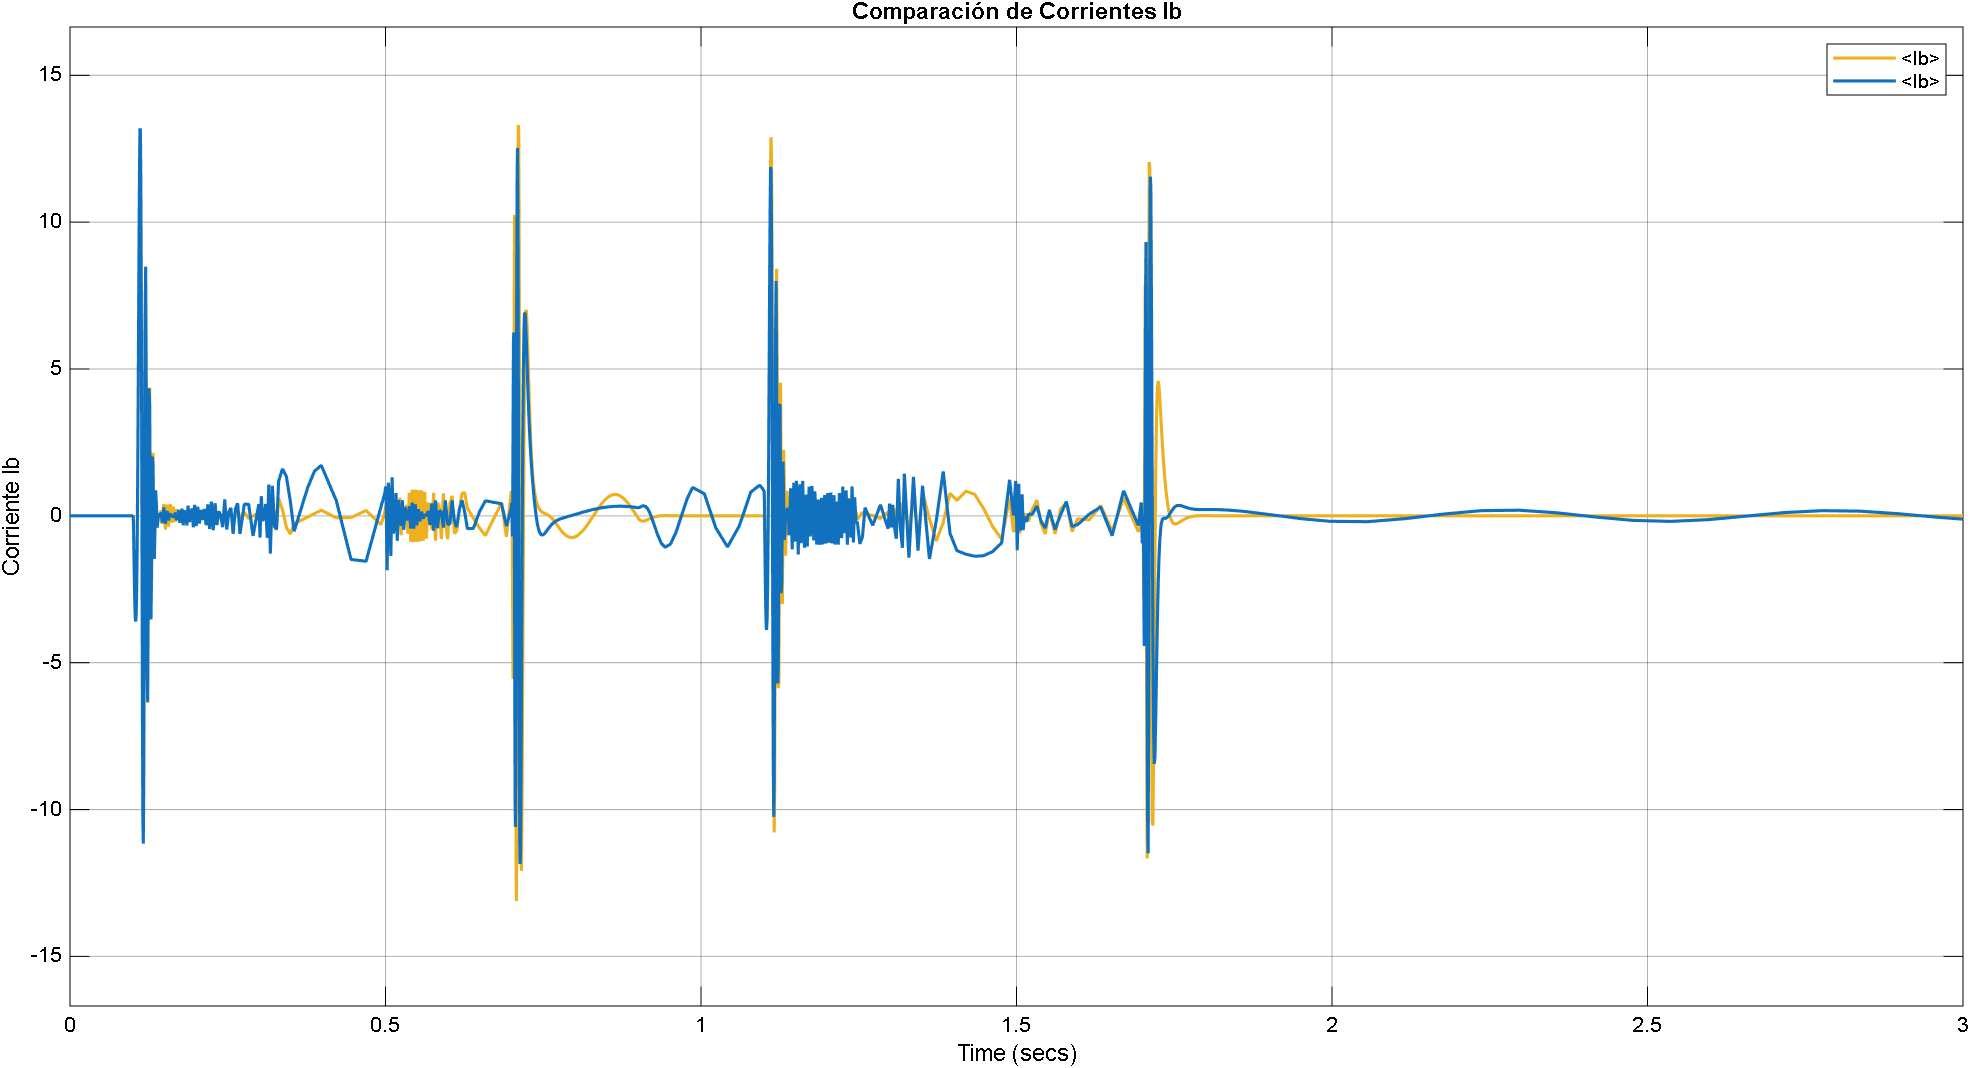
\includegraphics[width=0.6\linewidth]{attachments/Compa_NL_LTI_Ib.png}
    \caption{Corriente Ib respecto al Tiempo (Amarillo->LTI Aumentado; Azul-> NL con Ley}
    \label{fig:placeholder}
\end{figure}

\FloatBarrier
\begin{figure}[h]
    \centering
    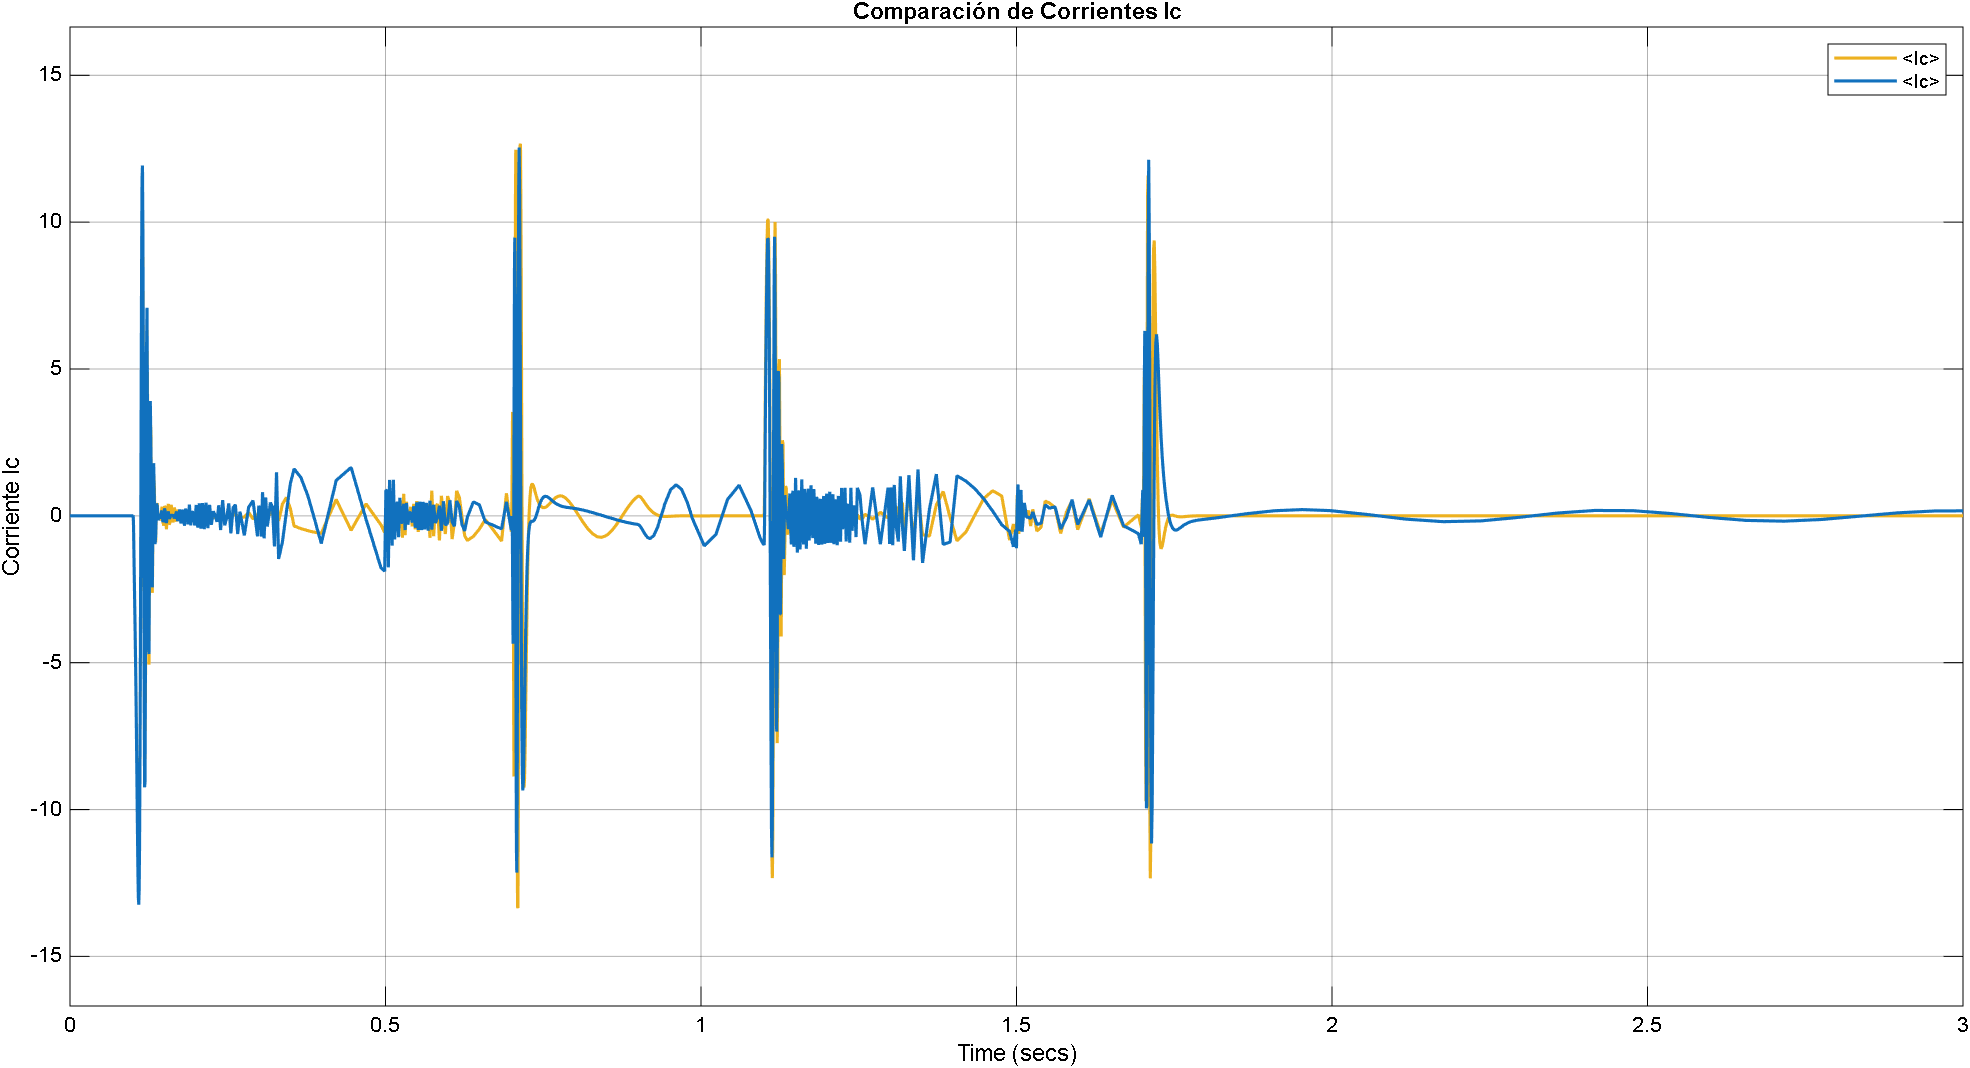
\includegraphics[width=0.6\linewidth]{attachments/Compa_NL_LTI_Ic.png}
    \caption{Corriente Ic respecto al Tiempo (Amarillo->LTI Aumentado; Azul-> NL con Ley}
    \label{fig:placeholder}
\end{figure}

\FloatBarrier
\begin{figure}[h]
    \centering
    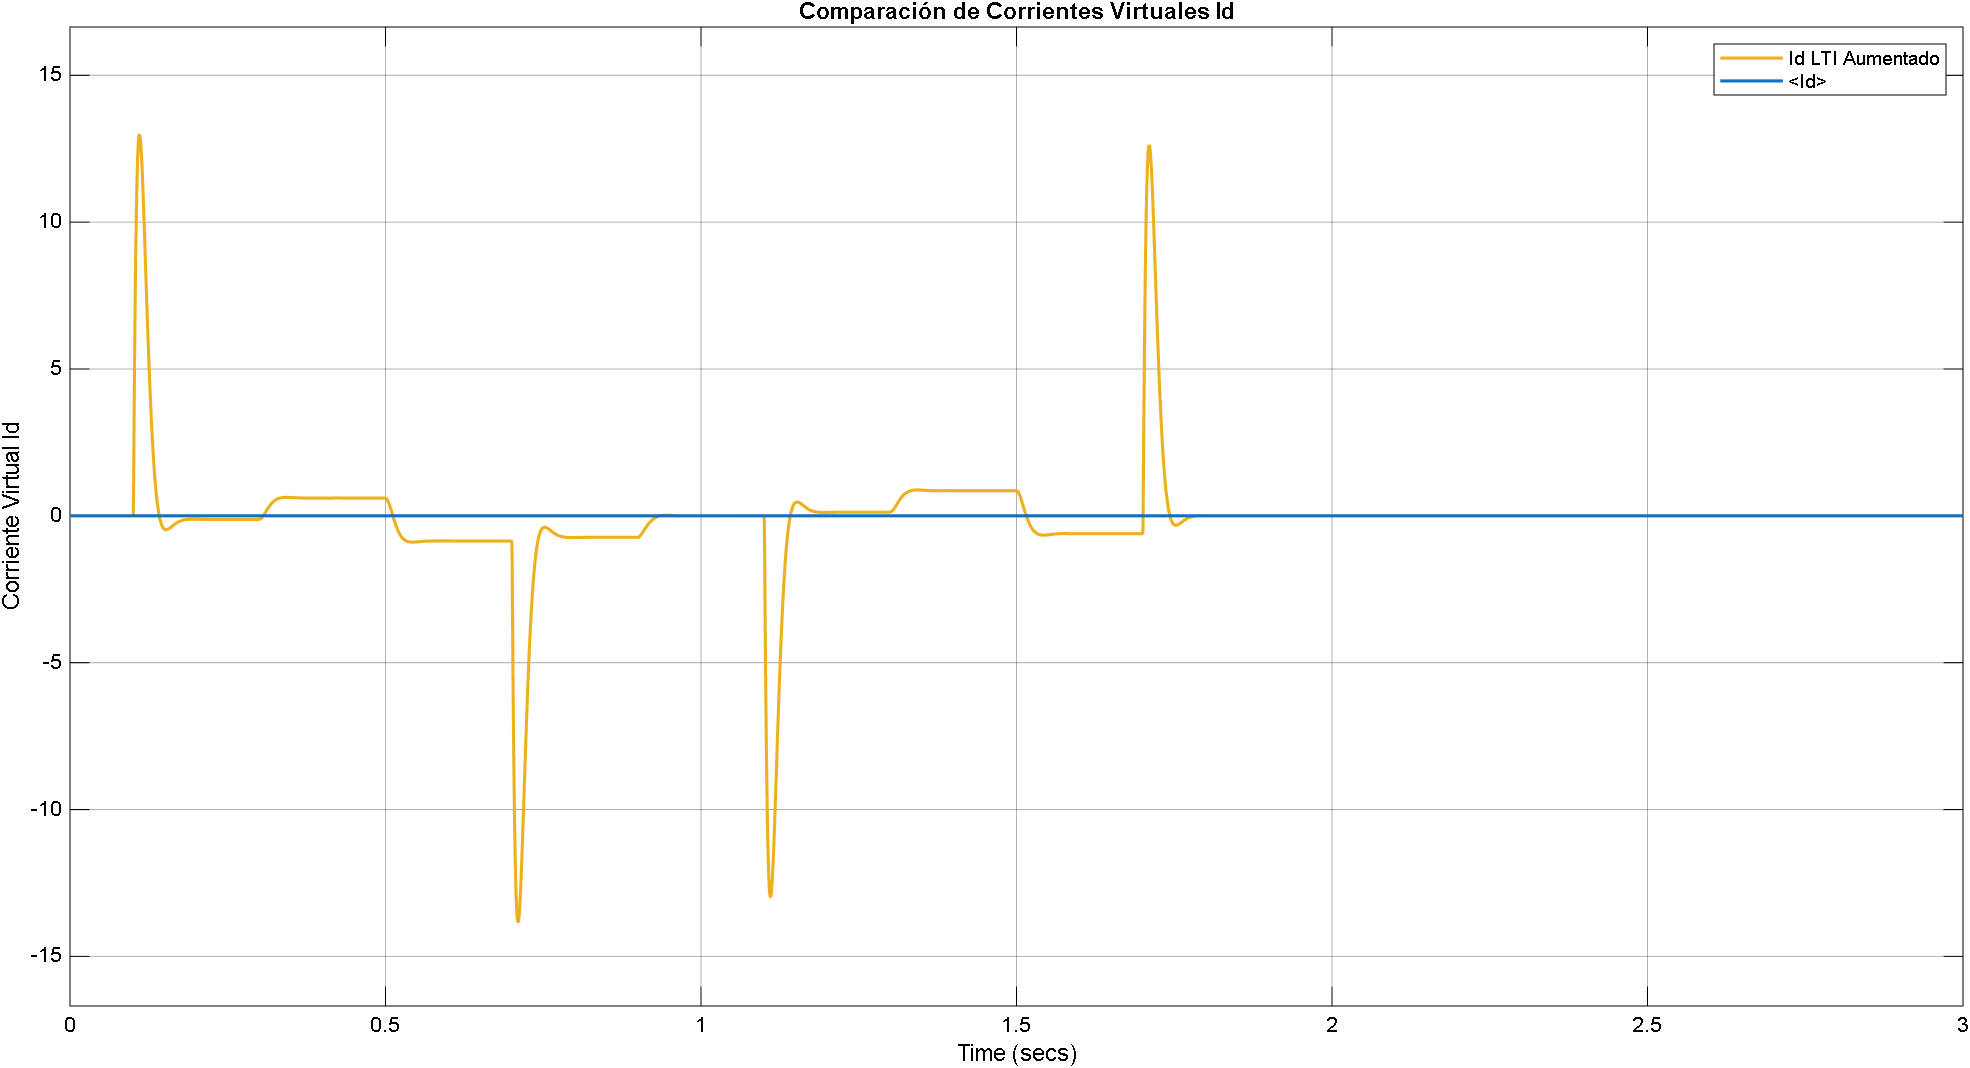
\includegraphics[width=0.6\linewidth]{attachments/Compa_NL_LTI_Id.png}
    \caption{Corriente Virtual Id}
    \label{fig:placeholder}
\end{figure}

\FloatBarrier
\begin{figure}[h]
    \centering
    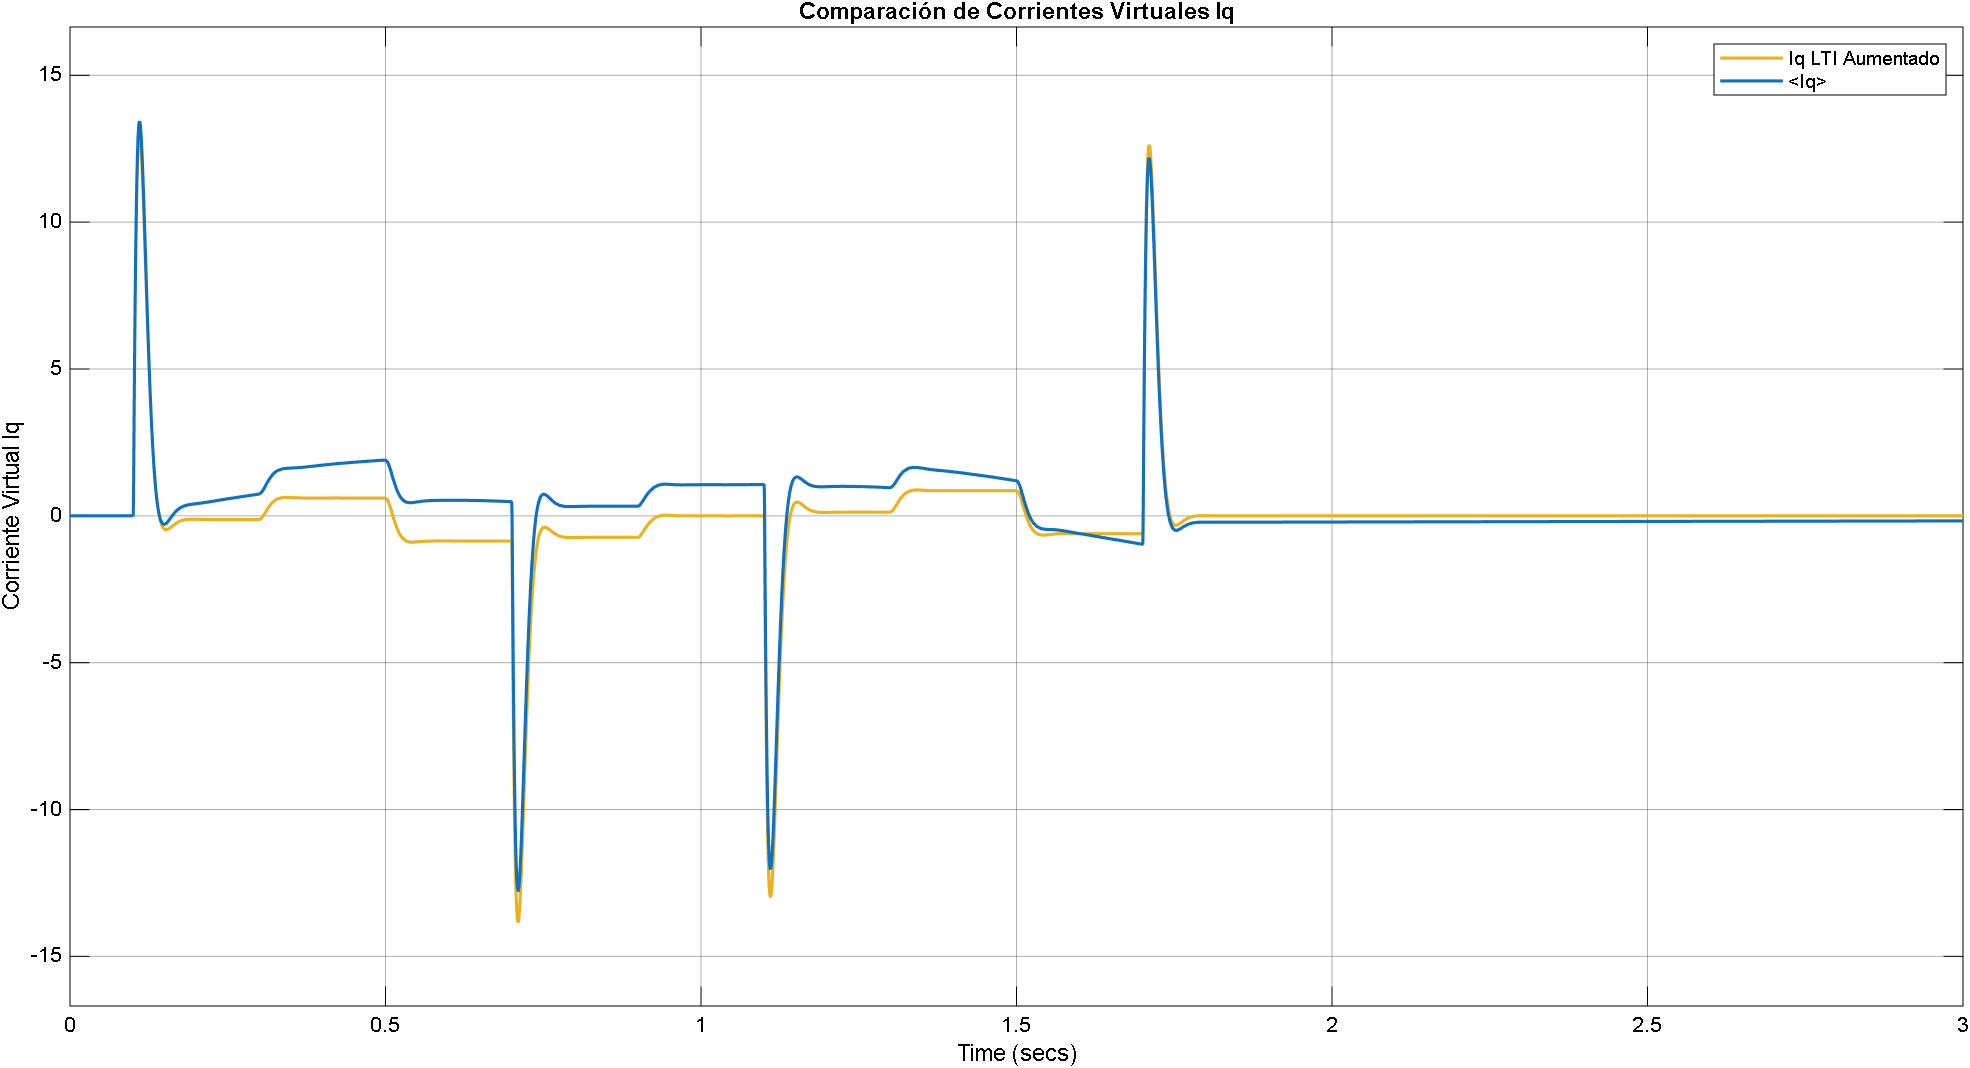
\includegraphics[width=0.6\linewidth]{attachments/Compa_NL_LTI_Iq.png}
    \caption{Corriente Virtual Iq}
    \label{fig:placeholder}
\end{figure}

\FloatBarrier
\begin{figure}[h]
    \centering
    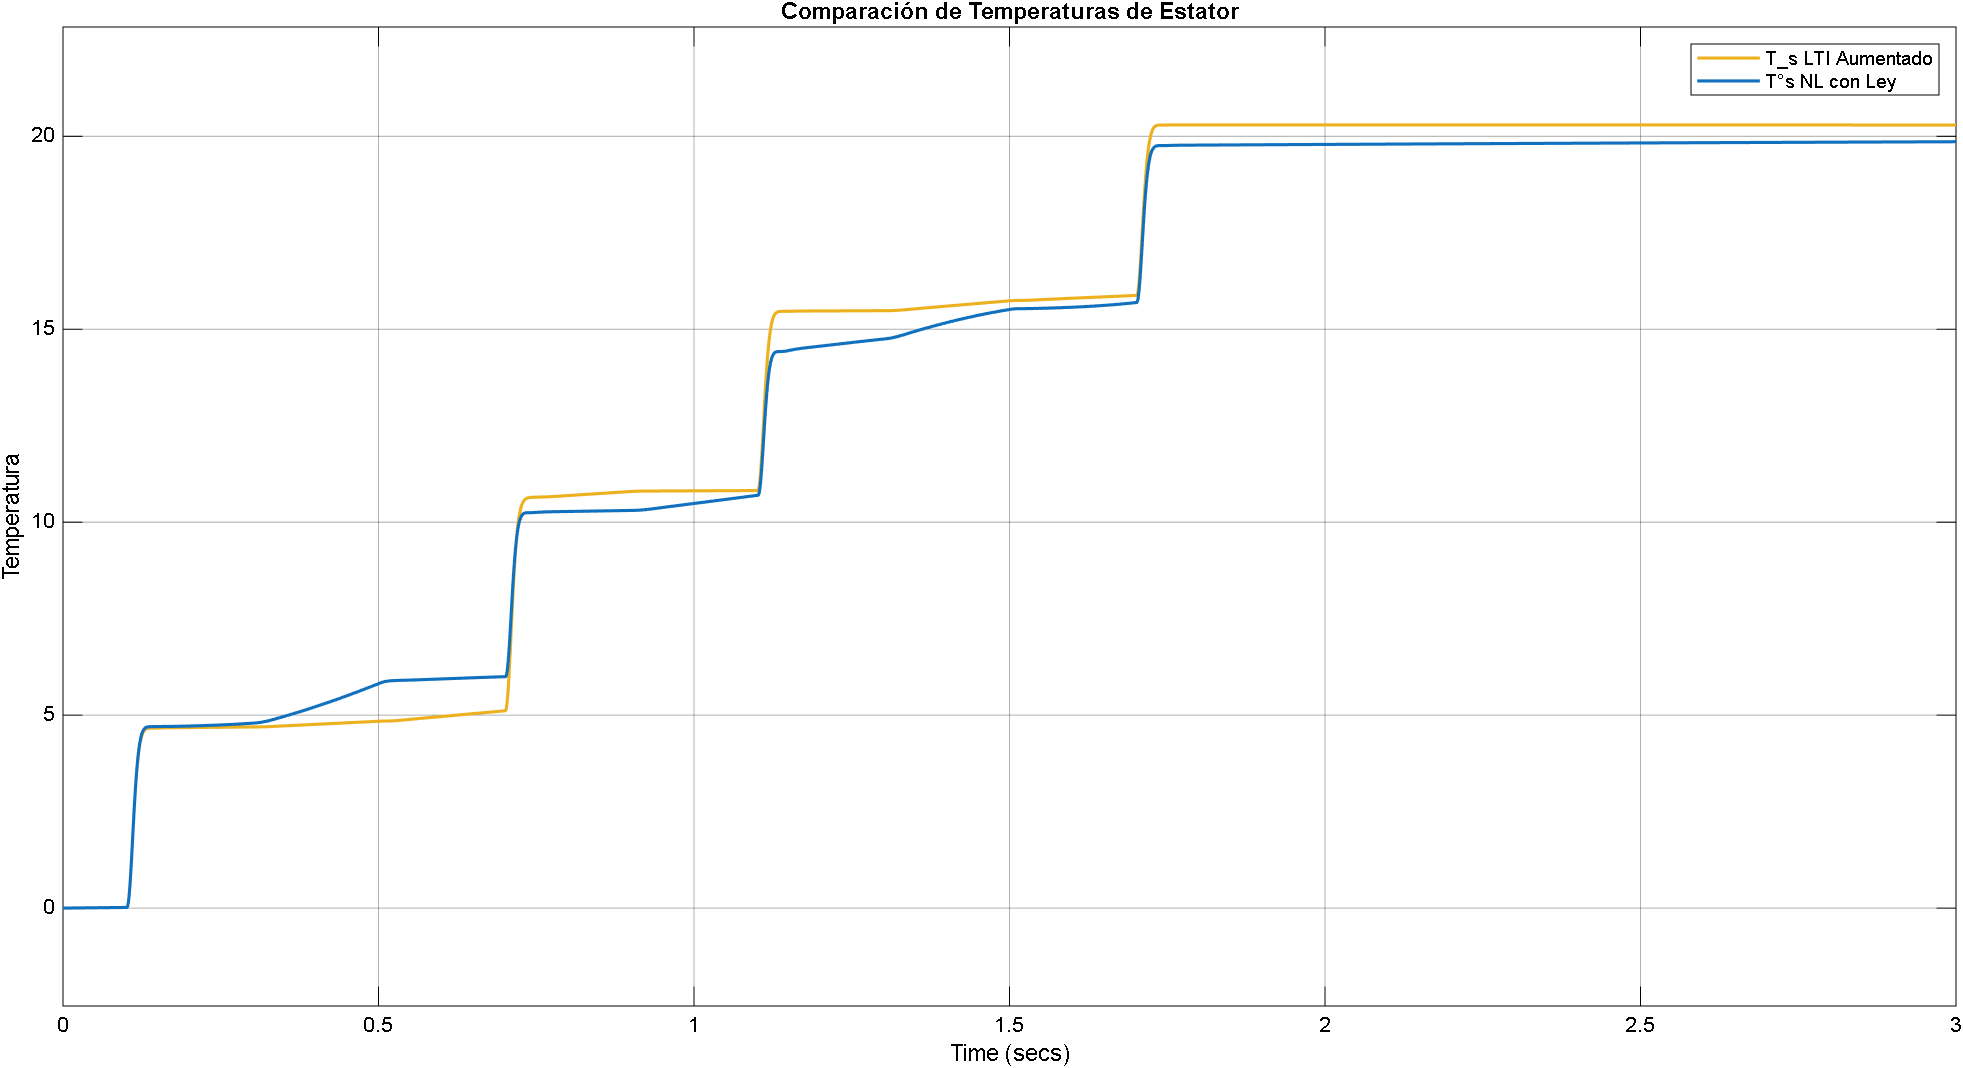
\includegraphics[width=0.6\linewidth]{attachments/Compa_NL_LTI_Temp_estator.png}
    \caption{Temperatura del Estator}
    \label{fig:placeholder}
\end{figure}
\FloatBarrier

\begin{figure}
    \centering
    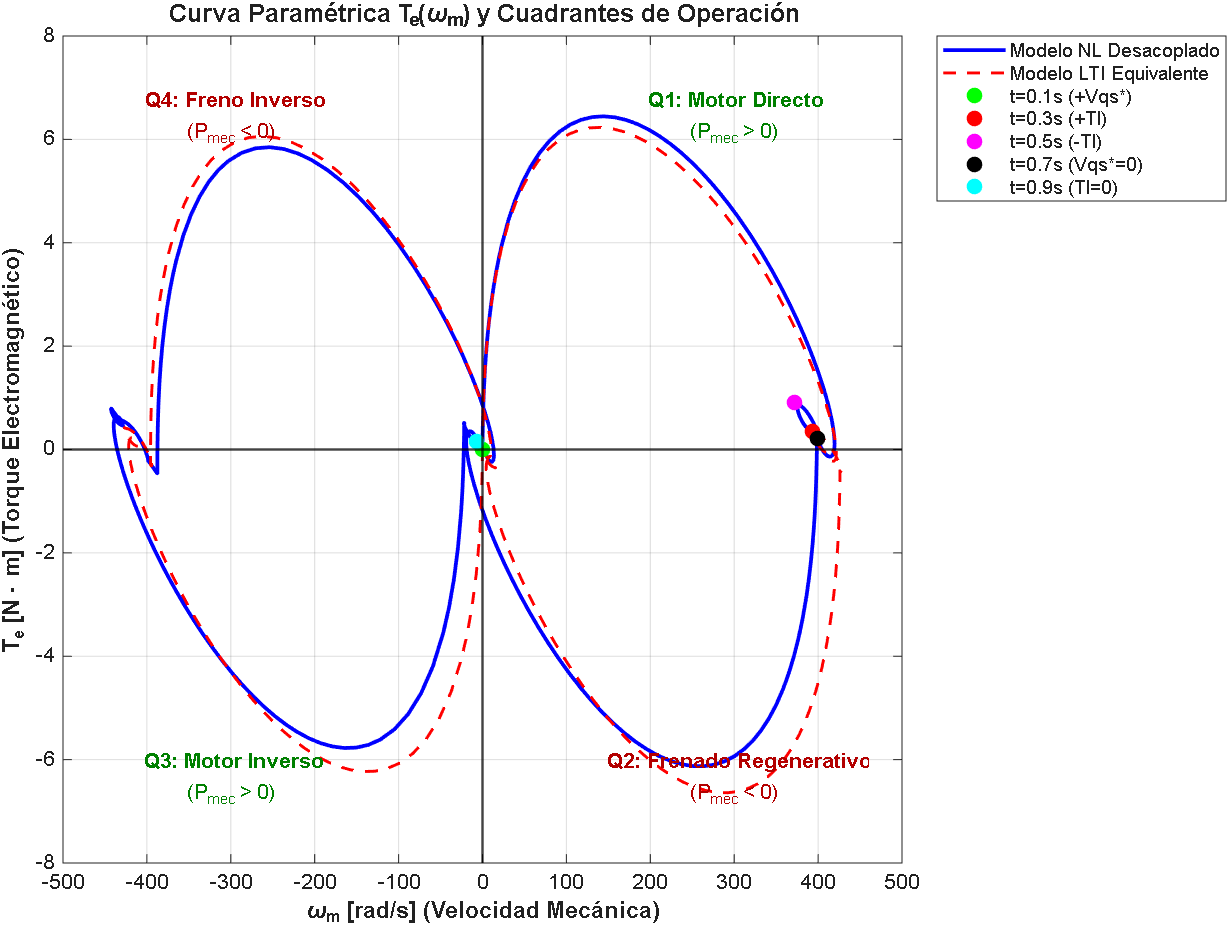
\includegraphics[width=0.75\linewidth]{attachments/Cuadrantes de Operación.png}
    \caption{curvas paramétricas torque vs velocidad}
    \label{fig:placeholder}
\end{figure}



% =========================================================================
% TABLA 1: Velocidad Mecánica \omega_m - Modelo NL Desacoplado
% =========================================================================
\begin{table}[htbp]
\centering
\caption{Resultados dinámicos de la velocidad $\omega_m$ (Modelo NL Desacoplado)}
\begin{tabular}{|c|c|c|c|c|c|}
\hline
$t_{event}\text{ (s)}$ & $y_0\text{ (rad/s)}$ & $y_f\text{ (rad/s)}$ & $\text{RiseTime}_{10-90}\text{ (s)}$ & $\text{SettlingTime}_{\pm 1\%}\text{ (s)}$ & $\text{Overshoot (\%)} $ \\
\hline
0.1 & $1.963 \times 10^{-9}$ & 393.090  & 0.0180 & 0.1389 & 6.76  \\
\hline
0.3 & 391.610                & 369.990  & 0.1274 & 0.1906 & 0.00  \\
\hline
0.5 & 371.360                & 398.720  & 0.0144 & 0.1870 & 4.22  \\
\hline
0.7 & 398.710                & -6.724   & 0.0196 & 0.0580 & 3.15  \\
\hline
0.9 & -7.499                 & 3.702    & 0.0026 & 1.9054 & 89.16 \\
\hline
\end{tabular}
\label{tab:dinamica_wm_NL}
\end{table}
\FloatBarrier
% =========================================================================
% TABLA 2: Velocidad Mecánica \omega_m - Modelo LTI Aumentado
% =========================================================================
\begin{table}[htbp]
\centering
\caption{Resultados dinámicos de la velocidad $\omega_m$ (Modelo LTI Aumentado)}
\begin{tabular}{|c|c|c|c|c|c|}
\hline
$t_{event}\text{ (s)}$ & $y_0\text{ (rad/s)}$ & $y_f\text{ (rad/s)}$ & $\text{RiseTime}_{10-90}\text{ (s)}$ & $\text{SettlingTime}_{\pm 1\%}\text{ (s)}$ & $\text{Overshoot (\%)} $ \\
\hline
0.1 & $1.963 \times 10^{-9}$ & 410.860                & 0.0203 & 0.0585 & 2.64    \\
\hline
0.3 & 409.500                & 395.620                & 0.0153 & 0.0530 & 4.39    \\
\hline
0.5 & 397.030                & 426.100                & 0.0154 & 0.0525 & 4.15    \\
\hline
0.7 & 426.080                & 15.239                 & 0.0203 & 0.0584 & 2.64    \\
\hline
0.9 & 14.465                 & $5.280 \times 10^{-13}$ & 0.0171 & 0.8958 & 2950.40 \\
\hline
\end{tabular}
\label{tab:dinamica_wm_LTI}
\end{table}
\FloatBarrier
% =========================================================================
% TABLA 3: Corriente de Estator i_qs^r - Modelo NL Desacoplado
% =========================================================================
\begin{table}[htbp]
\centering
\caption{Resultados dinámicos de la corriente $i_{qs}^r$ (Modelo NL Desacoplado)}
\begin{tabular}{|c|c|c|c|c|c|}
\hline
$t_{event}\text{ (s)}$ & $y_0\text{ (A)}$ & $y_f\text{ (A)}$ & $\text{RiseTime}_{10-90}\text{ (s)}$ & $\text{SettlingTime}_{\pm 1\%}\text{ (s)}$ & $\text{Overshoot (\%)} $ \\
\hline
0.1 & $2.053 \times 10^{-6}$ & 0.740  & 0.0004 & 0.1968 & 1715.40  \\
\hline
0.3 & 0.757                 & 1.898  & 0.1212 & 0.1904 & 0.00     \\
\hline
0.5 & 1.891                 & 0.481  & 0.0194 & 0.1854 & 2.41     \\
\hline
0.7 & 0.426                 & 0.329  & 0.0001 & 0.1573 & 13484.00 \\
\hline
0.9 & 0.333                 & -0.175 & 0.0002 & 1.9112 & 2334.60  \\
\hline
\end{tabular}
\label{tab:dinamica_iqs_NL}
\end{table}
\FloatBarrier
% =========================================================================
% TABLA 4: Corriente de Estator i_qs^r - Modelo LTI Aumentado
% =========================================================================
\begin{table}[htbp]
\centering
\caption{Resultados dinámicos de la corriente $i_{qs}^r$ (Modelo LTI Aumentado)}
\begin{tabular}{|c|c|c|c|c|c|}
\hline
$t_{event}\text{ (s)}$ & $y_0\text{ (A)}$ & $y_f\text{ (A)}$ & $\text{RiseTime}_{10-90}\text{ (s)}$ & $\text{SettlingTime}_{\pm 1\%}\text{ (s)}$ & $\text{Overshoot (\%)} $ \\
\hline
0.1 & $2.053 \times 10^{-6}$ & -0.125                  & 0.0010 & 0.1177 & 276.65  \\
\hline
0.3 & -0.114                 & 0.606                   & 0.0204 & 0.0601 & 3.30    \\
\hline
0.5 & 0.596                  & -0.857                  & 0.0202 & 0.0584 & 2.64    \\
\hline
0.7 & -0.912                 & -0.732                  & 0.0014 & 0.1153 & 191.99  \\
\hline
0.9 & -0.727                 & $-4.598 \times 10^{-14}$ & 0.0225 & 0.8836 & 1737.30 \\
\hline
\end{tabular}
\label{tab:dinamica_iqs_LTI}
\end{table}
\FloatBarrier
\clearpage

% ============================================================================= %
% [Start 10/11/2026]

\section{Diseño, análisis y simulación con controlador de movimiento en
cascada con modulador de torque equivalente (control vectorial)}

En la sección anterior se estudió la planta a lazo abierto mediante los modelos LPV y LTI equivalente, y se analizaron sus propiedades de estabilidad, controlabilidad y observabilidad. A continuación, se aborda el diseño de una estrategia de control a lazo cerrado basada en el \textbf{control en cascada}. Esta estructura aprovecha la diferencia entre las constantes de tiempo de los subsistemas eléctrico y mecánico para organizar el control en lazos con distintas velocidades de respuesta.

La estrategia se organiza en dos lazos principales:

\begin{itemize}
    \item \textbf{Lazo interno (rápido):} Controla la dinámica eléctrica de la máquina, regulando las corrientes y, por consiguiente, el torque electromagnético. Su respuesta debe ser más rápida que la del lazo externo.
    \item \textbf{Lazo externo (lento):} Controla la dinámica mecánica del accionamiento para satisfacer las consignas de posición y velocidad frente a los requerimientos de la carga.
\end{itemize}
    
Para implementar esta estrategia, el sistema de control se estructura en los siguientes bloques funcionales:

\begin{itemize}
    \item \textbf{Modulador de torque equivalente (lazo interno):} Vincula la consigna de torque con las variables eléctricas de la máquina. Mediante la generación de referencias de corriente, su regulación y la compensación de los acoplamientos, determina las tensiones necesarias en los ejes rotativos para alcanzar el torque solicitado.
    \item \textbf{Modulador de tensión (inversor):} Constituye la etapa de potencia que convierte las señales de control de tensión, calculadas por el modulador de torque, en tensiones trifásicas aplicadas a los bornes del estator.
    \item \textbf{Controlador de movimiento (lazo externo):} Emplea un esquema PID que recibe las consignas de movimiento y genera la referencia de torque a partir de los errores de seguimiento.
    \item \textbf{Observador de estado de orden reducido:} Estima las variables mecánicas no medidas, como la velocidad del rotor, a partir de la posición medida y del modelo del sistema. De esta manera, proporciona la información necesaria para la realimentación sin recurrir a la derivación directa de la señal de posición, sensible al ruido de medición.
\end{itemize}




% ---------------------------------------------------------------------------- %
\subsection{Modulador de torque equivalente}
El modulador de torque equivalente recibe una consigna de torque y calcula las tensiones que deben aplicarse a la máquina para producirlo. Su diseño combina la compensación de las realimentaciones naturales de la planta con la regulación de las corrientes virtuales.

El desarrollo se divide en tres etapas:
\begin{itemize}
    \item Modulación de tensiones y desacoplamiento por realimentación no lineal.
    \item Diseño de los lazos de control de corrientes virtuales con desacoplamiento mutuo y respecto de la velocidad angular.
    \item Compensación del torque de carga por gravedad.
\end{itemize}

En conjunto, estas etapas permiten pasar de la consigna de torque a las referencias de corriente y, a partir de ellas, a las tensiones virtuales que se aplican a la planta global no lineal.

% Realizar gráfico:

% Consigna Torque ->_{define} Consigna Corriente Virtual Q ->_{define} Consigna de Tensiones Virtuales dq0 ->_{obtiene} Tensiones Virtuales dq0 a aplicar a la planta Global No Lineal. 

\subsubsection{Modulación de tensiones y desacoplamiento por realimentación no lineal}

Las tensiones virtuales $v_{ds}^{r}(t)$, $v_{qs}^{r}(t)$ y $v_{0s}^{r}(t)$ son las entradas de control del subsistema electromagnético y actúan directamente sobre la dinámica de las corrientes virtuales. Estas corrientes determinan el torque electromagnético que, a su vez, modifica la velocidad y la posición angular del accionamiento. Por lo tanto, el diseño comienza por las ecuaciones de las corrientes:

\begin{align*}
\frac{di_{ds}^{r}(t)}{dt} & = \frac{1}{L_{d}} \left[ v_{ds}^{r}(t) - R_{s} \Big( T_{s}^{\circ} (t) \Big) i_{ds}^{r}(t) + L_{q}i_{qs}^{r}(t) \omega_{m}(t)P_{p}  \right]  \\
\frac{di_{qs}^{r}(t)}{dt}  & = \frac{1}{L_{q} } \left[ v_{qs}^{r}(t) - R_{s} \Big( T_{s}^{\circ} (t) \Big) i_{qs}^{r}(t) - \big[ \lambda_{m}^{'r} + L_{d} i_{ds}^{r}(t) \big] \omega_{m}(t)P_{p} \right]  \\
\frac{di_{0s}^{r}(t)}{dt} & = \frac{1}{ L_{ls} } \left[ v_{0s}^{r}(t) - R_{s} \Big( T_{s}^{\circ} (t) \Big) i_{0s}^{r}(t) \right]
\end{align*}

Para compensar las caídas resistivas y los términos de acoplamiento y fuerza contraelectromotriz, se proponen las siguientes tensiones virtuales:
\begin{align}
v_{ds}^{r}(t) & = v_{ds}^{*r}(t) + R_{s} \Big( T_{s}^{\circ} (t) \Big) i_{ds}^{r}(t) - L_{q}i_{qs}^{r}(t) \omega_{m}(t)P_{p}    \\
v_{qs}^{r}(t) & = v_{qs}^{*r}(t) + R_{s} \Big( T_{s}^{\circ} (t) \Big) i_{qs}^{r}(t) + \big[ \lambda_{m}^{'r} + L_{d} i_{ds}^{r}(t) \big] \omega_{m}(t)P_{p}  \\
v_{0s}^{r}(t) & = v_{0s}^{*r}(t) + R_{s} \Big( T_{s}^{\circ} (t) \Big) i_{0s}^{r}(t) 
\end{align}

\noindent Las consignas de tensión se definen como:
\begin{description}[leftmargin=1.2cm, labelwidth=1cm]
    \item[$v_{ds}^{*r}(t)$] Consigna de tensión del eje directo.
    \item[$v_{qs}^{*r}(t)$] Consigna de tensión del eje en cuadratura.
    \item[$v_{0s}^{*r}(t)$] Consigna de tensión del eje cero.
\end{description}

Al sustituir estos valores de $v_{ds}^{r}(t)$, $v_{qs}^{r}(t)$ y $v_{0s}^{r}(t)$ en las ecuaciones dinámicas de las corrientes, se obtiene:

\begin{align*}
\frac{di_{ds}^{r}(t)}{dt} & = \frac{1}{L_{d}} \Bigg[ \Big( v_{ds}^{*r}(t) + \cancel{ R_{s} \Big( T_{s}^{\circ} (t) \Big) i_{ds}^{r}(t) } - \cancel{ L_{q}i_{qs}^{r}(t) \omega_{m}(t)P_{p} } \Big) - \cancel{ R_{s} \Big( T_{s}^{\circ} (t) \Big) i_{ds}^{r}(t) } + \cancel{ L_{q}i_{qs}^{r}(t) \omega_{m}(t)P_{p}  } \Bigg]  \\
\frac{di_{qs}^{r}(t)}{dt}  & = \frac{1}{L_{q} } \Bigg[ \Big( v_{qs}^{*r}(t) +\cancel{  R_{s} \Big( T_{s}^{\circ} (t) \Big) i_{qs}^{r}(t) } +\cancel{  \big[ \lambda_{m}^{'r} + L_{d} i_{ds}^{r}(t) \big] \omega_{m}(t)P_{p}  } \Big) - \cancel{ R_{s} \Big( T_{s}^{\circ} (t) \Big) i_{qs}^{r}(t) } - \cancel{ \big[ \lambda_{m}^{'r} + L_{d} i_{ds}^{r}(t) \big] \omega_{m}(t)P_{p}  }\Bigg]  \\
\frac{di_{0s}^{r}(t)}{dt} & = \frac{1}{ L_{ls} } \Bigg[ \Big( v_{0s}^{*r}(t) + \cancel{ R_{s} \Big( T_{s}^{\circ} (t) \Big) i_{0s}^{r}(t) }  \Big) -\cancel{  R_{s} \Big( T_{s}^{\circ} (t) \Big) i_{0s}^{r}(t) } \Bigg]
\end{align*}

Con esta compensación, las dinámicas de las corrientes virtuales se simplifican a:
\begin{align}
\frac{di_{ds}^{r}(t)}{dt} & = \frac{1}{L_{d}} v_{ds}^{*r}(t)  \\
\frac{di_{qs}^{r}(t)}{dt}  & = \frac{1}{L_{q} } v_{qs}^{*r}(t) \\
\frac{di_{0s}^{r}(t)}{dt} & = \frac{1}{ L_{ls} } v_{0s}^{*r}(t) 
\end{align}

% > Comparar la diferencia entre usar $R_{s}(T^{\circ}_{s}(t))$ y utilizar $R_{s}^{\ell}$.

% Realizar gráficos de comparaciones

\subsubsection{Diseño de los lazos de control de corrientes virtuales con desacoplamiento mutuo y respecto de la velocidad angular}

Una vez compensadas las realimentaciones naturales, cada corriente virtual se regula mediante un controlador proporcional al error de seguimiento. El procedimiento es análogo para los ejes directo, en cuadratura y cero; por ello, se presenta primero un desarrollo general, sin subíndices.

Como criterio de diseño, se fija el polo de cada lazo de corriente en $p=-5000\;\frac{\text{rad}}{\text{seg}}$. Para la respuesta de primer orden resultante, esta elección corresponde a un ancho de banda de $|p|=2\pi f_c=5000\;\frac{\text{rad}}{\text{seg}} \implies f_c \approx 796\; \textbf{Hz}$. La consigna de tensión se define mediante la ley proporcional:
\[
v^{*}(t) = K_{p} \Big( i^{*}(t) -i(t) \Big)
\]
Al sustituir esta ley en la dinámica de corriente obtenida tras la compensación, resulta:
\[
\frac{di(t)}{dt} = \frac{1}{L} v^{*}(t) =  \frac{1}{L} K_{p} \Big( i^{*}(t) -i(t) \Big)
\]
Aplicando la transformada de Laplace con condiciones iniciales nulas y agrupando los términos en el dominio complejo $s$, se obtiene la función de transferencia de seguimiento de corriente del lazo cerrado:
\begin{align*}
\frac{di(t)}{dt}  & = \frac{K_{p}}{L}  \Big( i^{*}(t) -i(t) \Big) \\
sI & = \frac{K_{p}}{L} \Big( I^{*} - I \Big) \\
\Big( s + \frac{K_{p}}{L} \Big) I & = \frac{K_{p}}{L} I^{*} \\
\frac{I}{I^{*}} & = \frac{\frac{K_{p}}{L}}{s+\frac{K_{p}}{L}}=\frac{1}{\frac{L}{K_{p}}s+1}
\end{align*}

El lazo presenta un polo en $p=-\frac{K_{p}}{L}$. La ganancia $K_p$ tiene dimensión de resistencia, $[\Omega]$, y se denota mediante la letra R para cada eje. Así, las funciones de transferencia particulares son:
\begin{align}
\frac{I_{d}}{I_{d}^{*}} & = \frac{1}{\frac{L_d}{R_{d}}s+1} \\
\frac{I_{q}}{I_{q}^{*}} & = \frac{1}{\frac{L_q}{R_{q}}s+1} \\
\frac{I_{0}}{I_{0}^{*}} & = \frac{1}{\frac{L_{ls}}{R_{0}}s+1}
\end{align}

Las ganancias necesarias para ubicar los tres polos en el valor especificado se calculan como:
\[
p = -\frac{R}{L} \implies \begin{cases}
R_{d} & = 5000 L_{d} = 33\; [\Omega] \\
R_{q} & = 5000 L_{q} = 29\; [\Omega]\\
R_{0} & = 5000 L_{ls} = 4\; [\Omega]
\end{cases}
\]


% > ¿Qué provoca agregar acción integral? Investigar sus consecuencias.

\subsubsection{Compensación del torque de carga por gravedad}

El paso siguiente consiste en definir las referencias de corriente a partir de la consigna de torque. Como condición inicial de diseño, se adoptan las siguientes consignas:
\begin{align*}
i_{ds}^{*r}(t) & = 0 \\
i_{qs}^{*r}(t) & \neq 0 \\
i_{0s}^{*r}(t) & = 0
\end{align*}

La corriente en cuadratura permite regular el torque útil, mientras que la corriente directa modifica el campo magnético y la corriente de secuencia cero solo introduce pérdidas. Aunque puede considerarse el caso $i_{ds}^{*r}(t) \neq 0$ para debilitar o reforzar el campo (\textit{field weakening} o \textit{field forcing}, según el signo de la corriente), el estudio comienza con $i_{ds}^{*r}(t) = 0$.

Para compensar la fricción viscosa equivalente y el torque gravitatorio de la carga, se retoma la ecuación de la velocidad angular del motor:

\[
\frac{d\omega_{m}(t)}{dt} = \frac{1}{J_{eq}} \Bigg[ \frac{3}{2}P_{p} \lambda_{m}^{'r} i_{qs}^{r}(t) + \frac{3}{2} P_{p} \Big( L_{d} - L_{q} \Big) i_{qs}^{r}(t) i_{ds}^{r}(t) - b_{eq}  \omega_{m}(t)   - \frac{1}{r} T_{dl}(t) - \frac{k_{l}g}{r} \sin \left(  \frac{1}{r} \theta_{m}(t) \right) \Bigg]
\]

El objetivo es obtener la siguiente relación entre la consigna de torque y la aceleración angular:
\[
\frac{d\omega_{m}(t)}{dt} = \frac{T_{m}^{*}(t)}{J_{eq}} 
\]

El torque $T_{dl}$ constituye una \textbf{perturbación de la carga mecánica}, cuya magnitud y evolución temporal se consideran desconocidas para el controlador. Por esta razón, no se incorpora a la ley de compensación. El torque solicitado al motor incluye la consigna de movimiento y las compensaciones viscosa y gravitatoria:

\begin{align*}
T_{m}(t) & = T_{m}^{*}(t) +b_{eq}\omega_{m}(t) + \frac{k_{l}g}{r} \sin \left( \frac{1}{r} \theta_{m}(t)  \right) \\
T_{m}(t) & \approx \frac{3}{2}P_{p} \Big[ \lambda_{m}^{'r} + \Big( L_{d}-L_{q} \Big)i_{ds}^{r}(t) \Big] i_{qs}^{*r}(t)
\end{align*}

Al despejar la referencia de corriente en cuadratura, se obtiene:

$$
i_{qs}^{*r}(t) = \frac{T_{m}^{*}(t) +b_{eq}\omega_{m}(t) + \frac{k_{l}g}{r} \sin \left( \frac{1}{r} \theta_{m}(t)  \right)}{\frac{3}{2}P_{p} \Big[ \lambda_{m}^{'r} + \Big( L_{d}-L_{q} \Big)i_{ds}^{r}(t) \Big]}
$$




% ---------------------------------------------------------------------------- %
\subsection{Controlador externo de movimiento: posición y velocidad}

El controlador externo de movimiento se diseña para recibir consignas de posición o velocidad angular mediante el método de sintonía serie con acción integral. Se adoptan como parámetros de diseño $\zeta = 0.75$ y $\omega_{n}=800 \frac{rad}{seg}$, y se consideran los valores nominales de los parámetros de carga $J_{l}$ y $b_{l}$, sin incluir la incertidumbre de los datos.

La consigna de torque se genera mediante una ley PID que combina los errores de posición y velocidad con la integral del error de posición. En el dominio de Laplace $s$, se expresa como:
\begin{align*}
T_{m}^{*}(s) & = K_{p}^{\text{mov}}e_{\theta}(s) + K_{d}^{\text{mov}} e_{\omega}(s) + K_{i}^{\text{mov}} \frac{1}{s} e_{\theta}(s) \\
 & = \Big[  K_{p}^{\text{mov}} + sK_{d}^{\text{mov}} + \frac{1}{s}K_{i}^{\text{mov}} \Big] e_{\theta}(s) \\
 & = \Big[  K_{p}^{\text{mov}} + sK_{d}^{\text{mov}} + \frac{1}{s}K_{i}^{\text{mov}} \Big] \Big( \Theta^{*}_{m}(s) - \Theta_{m}(s) \Big) % crear referencia \tag o lo que sea
\end{align*}

La dinámica mecánica resultante de la compensación del modulador de torque equivalente se describe mediante:
\[
\frac{d\omega_{m}(t)}{dt} = \frac{1}{J_{eq}} \Big[ T_{m}^{*}(t)- \frac{1}{r} T_{dl}(t) \Big]
\]

Con condiciones iniciales nulas, su transformación al dominio de Laplace $s$ permite escribir:
\begin{align*}
s\Omega_{m}(s)  & = \frac{1}{J_{eq}} \Big[ T_{m}^{*}(s)- \frac{1}{r} T_{dl}(s) \Big] \\ 
s^{2}\Theta_{m}(s)  & = \frac{1}{J_{eq}} \Big[ T_{m}^{*}(s)- \frac{1}{r} T_{dl}(s) \Big] \\
s^{2}J_{eq} \Theta_{m}(s)  & = T_{m}^{*}(s)- \frac{1}{r} T_{dl}(s) 
\end{align*}

Al sustituir la consigna de torque por la ley PID anterior, %referencia a la expresión de consigna T*m
resulta:
\[
s^{2}J_{eq} \Theta_{m}(s) = \Big[  K_{p}^{\text{mov}} + sK_{d}^{\text{mov}} + \frac{1}{s}K_{i}^{\text{mov}} \Big] \Big( \Theta^{*}_{m}(s) - \Theta_{m}(s) \Big) - \frac{1}{r} T_{dl}(s) 
\]
Agrupando los términos que dependen del ángulo $\Theta_m(s)$, se obtiene:
\[
\Big[ s^{2}J_{eq} + sK_{d}^{\text{mov}} + K_{p}^{\text{mov}}  + \frac{1}{s}K_{i}^{\text{mov}} \Big] \Theta_{m}(s) = \Big[  K_{p}^{\text{mov}} + sK_{d}^{\text{mov}} + \frac{1}{s}K_{i}^{\text{mov}} \Big] \Theta^{*}_{m}(s) - \frac{1}{r} T_{dl}(s) 
\]

Para eliminar las potencias negativas de $s$, se multiplican ambos miembros de la igualdad por $s$:

\[
\Big[ s^{3}J_{eq} + s^{2}K_{d}^{\text{mov}} + sK_{p}^{\text{mov}}  + K_{i}^{\text{mov}} \Big] \Theta_{m}(s) = \Big[  s^{2}K_{d}^{\text{mov}} + sK_{p}^{\text{mov}} + K_{i}^{\text{mov}} \Big] \Theta^{*}_{m}(s) - \frac{s}{r} T_{dl}(s) 
\]

Finalmente, al despejar la posición angular, resulta:
\[
\Theta_{m}(s) = \frac{  s^{2}K_{d}^{\text{mov}} + sK_{p}^{\text{mov}} + K_{i}^{\text{mov}} }{ s^{3}J_{eq} + s^{2}K_{d}^{\text{mov}} + sK_{p}^{\text{mov}}  + K_{i}^{\text{mov}} } \Theta^{*}_{m}(s) - \frac{\frac{s}{r}}{ s^{3}J_{eq} + s^{2}K_{d}^{\text{mov}} + sK_{p}^{\text{mov}}  + K_{i}^{\text{mov}} } T_{dl}(s) 
\]

Esta relación permite distinguir la contribución de la consigna de posición $\Theta_{m}^{*}(s)$ y la del torque perturbador $T_{dl}(s)$ a la respuesta del ángulo motor $\Theta_{m}(s)$. Las funciones de transferencia correspondientes, considerando nula la otra entrada en cada caso, son:

\begin{align}
G_{\Theta^{*}_{m}}(s) & = \frac{\Theta_{m}(s)}{\Theta^{*}_{m}(s) }  = \frac{  s^{2}K_{d}^{\text{mov}} + sK_{p}^{\text{mov}} + K_{i}^{\text{mov}} }{ s^{3}J_{eq} + s^{2}K_{d}^{\text{mov}} + sK_{p}^{\text{mov}}  + K_{i}^{\text{mov}} } \\
G_{T_{ld}}(s) & = \frac{\Theta_{m}(s)}{T_{dl}(s) } =  - \frac{\frac{s}{r}}{ s^{3}J_{eq} + s^{2}K_{d}^{\text{mov}} + sK_{p}^{\text{mov}}  + K_{i}^{\text{mov}} } 
\end{align}

Ambas funciones de transferencia comparten el siguiente polinomio característico:
\[
P(s) = s^{3}J_{eq} + s^{2}K_{d}^{\text{mov}} + sK_{p}^{\text{mov}}  + K_{i}^{\text{mov}} = s^{3}+ s^{2}\frac{K_{d}^{\text{mov}}}{J_{eq}} + s\frac{K_{p}^{\text{mov}}}{J_{eq}}  + \frac{K_{i}^{\text{mov}}}{J_{eq}}
\]

La asignación considera tres polos situados a una distancia de $800\;\frac{rad}{seg}$ del origen. Se elige un par de polos complejos conjugados definido por $\zeta=0.75$ y $\omega_{n}=800 \frac{rad}{seg}$, junto con un tercer polo real negativo cuyo módulo es $|p_{3}|=\omega_{n}=800 \frac{rad}{seg}$. El polinomio característico deseado resulta:

\begin{align}
P^{*}(s)  & = (s^{2}+2\zeta \omega_{n}s+\omega_{n}^{2})(s+\omega_{n})  \\
 \\
P^{*}(s)  & = s^{3} + \omega_{n} (2\zeta+1) s^{2} + \omega_{n}^{2} (2\zeta+1)s + \omega_{n}^{3}
\end{align}

Al igualar los coeficientes de los polinomios característicos y despejar las ganancias, % tag a la expresión correcta
considerando la inercia equivalente $J_{eq}$ para la carga máxima $m_{l} =1.5\;[\text{kg}]$, se obtienen los siguientes valores:

\[
\begin{cases}
\omega_{n} (2\zeta+1) & = \frac{K_{d}^{\text{mov}}}{J_{eq}} \\
\omega_{n}^{2} (2\zeta+1) & = \frac{K_{p}^{\text{mov}}}{J_{eq}} \\
\omega_{n}^{3} & = \frac{K_{i}^{\text{mov}}}{J_{eq}}
\end{cases} \quad  \implies \quad 
\begin{cases}
 K_{d}^{\text{mov}} & = \omega_{n} (2\zeta+1){J_{eq}} = 0.0917 \; \mathrm{\frac{Nm}{rad/s}}\\
K_{p}^{\text{mov}} & = \omega_{n}^{2} (2\zeta+1) {J_{eq}} = 73.3222 \mathrm{\frac{Nm}{rad}}\\
K_{i}^{\text{mov}} & = \omega_{n}^{3}{J_{eq}} = 23463 \mathrm{\frac{Nm}{rad\cdot s}}
\end{cases}
\]

% [TODO] Insertar imagen del bloque de Simulink

% ---------------------------------------------------------------------------- %
\subsection{Incorporación y diseño del observador de estado de orden reducido}

El observador se diseña a partir de las dinámicas de la posición angular $\theta_{m}$ y la velocidad angular $\omega_{m}$ del motor, considerando las compensaciones por realimentación no lineal introducidas en el modulador de torque. La posición angular es la salida medida del subsistema mecánico, cuyo modelo se expresa como:

\[
\left\{
\begin{aligned}
\frac{d \theta_{m}(t) }{dt} & = \omega_{m}(t) \\
\frac{d \omega_{m}(t) }{dt} & = \frac{1}{J_{eq}} \Big[ T_{m}^{*}(t)-\frac{1}{r}T_{dl}(t) \Big] \\
y & = \begin{bmatrix} 1 & 0 \end{bmatrix} \begin{bmatrix} \theta_{m}(t) \\ \omega_{m}(t) \end{bmatrix}
\end{aligned}
\right.
\]
La representación matricial correspondiente es:
\[
\left\{
\begin{aligned}
\begin{bmatrix} \frac{d \theta_{m}(t) }{dt} \\ \frac{d \omega_{m}(t) }{dt}  \end{bmatrix} 
 & = \begin{bmatrix} 0 & 1 \\0 & 0 \end{bmatrix} \begin{bmatrix} \theta_{m}(t) \\ \omega_{m}(t) \end{bmatrix} + \begin{bmatrix} 0 & 0 \\ \frac{1}{J_{eq}} & -\frac{1}{rJ_{eq}} \end{bmatrix} \begin{bmatrix} T^{*}_{m}(t) \\ T_{dl}(t) \end{bmatrix} \\
y & = \begin{bmatrix} 1 & 0 \end{bmatrix} \begin{bmatrix} \theta_{m}(t) \\ \omega_{m}(t) \end{bmatrix}
\end{aligned}
\right.
\]

Para construir el observador, se parte de la siguiente estructura matricial, que incorpora una corrección proporcional al error entre la salida medida y la estimada:

\[
\left\{
\begin{aligned}
\frac{d \mathbf{\hat{x}}(t) }{dt} & = \mathbf{A} \mathbf{\hat{x}}(t) + \mathbf{B}\mathbf{u}(t) + \mathbf{L}(\mathbf{y}-\mathbf{C}\mathbf{\hat{x}}) \\
\mathbf{\hat{y}} & = \mathbf{C} \mathbf{\hat{x}}
\end{aligned}
\right.
\]

A partir del modelo del subsistema mecánico definido por $\theta_{m}$ y $\omega_{m}$, se identifican las matrices:
\[
\mathbf{A}=\begin{bmatrix} 0 & 1 \\0 & 0 \end{bmatrix}
\]
\[
\mathbf{B} = \begin{bmatrix} 0 & 0 \\ \frac{1}{J_{eq}} & -\frac{1}{rJ_{eq}} \end{bmatrix}
\]
\[
\mathbf{C}=\begin{bmatrix} 1 & 0\end{bmatrix}
\]
La matriz de ganancias del observador debe tener dimensiones compatibles con el término de corrección:
\[
\mathbf{A}-\mathbf{L}\mathbf{C} \in \mathbb{R}^{2\times2} \implies \mathbf{L} \in \mathbb{R}^{2\times1}, \qquad \mathbf{L}=\begin{bmatrix} K_{\theta} \\ K_{\omega} \end{bmatrix}
\]

Al sustituir estas matrices en la estructura del observador, se obtiene:
\[
\left\{
\begin{aligned}
\begin{bmatrix} \frac{d \hat{\theta}_{m}(t) }{dt} \\ \frac{d \hat{\omega}_{m}(t) }{dt}  \end{bmatrix} 
 & = \begin{bmatrix} 0 & 1 \\0 & 0 \end{bmatrix} \begin{bmatrix} \hat{\theta}_{m}(t) \\ \hat{\omega}_{m}(t) \end{bmatrix} + \begin{bmatrix} 0 & 0 \\ \frac{1}{J_{eq}} & -\frac{1}{rJ_{eq}} \end{bmatrix} \begin{bmatrix} T^{*}_{m}(t) \\ T_{dl}(t) \end{bmatrix} + \begin{bmatrix} K_{\theta} \\ K_{\omega} \end{bmatrix} \Bigg( \theta_{m}(t) - \begin{bmatrix} 1 & 0 \end{bmatrix} \begin{bmatrix} \hat{\theta}_{m}(t) \\ \hat{\omega}_{m}(t) \end{bmatrix} \Bigg) \\
\hat{y} & = \begin{bmatrix} 1 & 0 \end{bmatrix} \begin{bmatrix} \hat{\theta}_{m}(t) \\ \hat{\omega}_{m}(t) \end{bmatrix}
\end{aligned}
\right.
\]

Se define el error de estimación como $\mathbf{\tilde{x}}=\mathbf{x}-\mathbf{\hat{x}}$ y se utiliza la relación $\mathbf{y} = \mathbf{C}\mathbf{x}$. Al restar las ecuaciones del observador % hacer referencia a la ecuación del modelo reducido de la planta
de las ecuaciones de la planta, % hacer referencia a la ecuación del modelo del observador de estado
se obtiene el siguiente modelo del error:

\[
\left\{
\begin{aligned}
\begin{bmatrix} \frac{d \tilde{\theta}_{m}(t) }{dt} \\ \frac{d \tilde{\omega}_{m}(t) }{dt}  \end{bmatrix} 
 & = \begin{bmatrix} 0 & 1 \\0 & 0 \end{bmatrix} \begin{bmatrix} \tilde{\theta}_{m}(t) \\ \tilde{\omega}_{m}(t) \end{bmatrix} - \begin{bmatrix} K_{\theta} \\ K_{\omega} \end{bmatrix} \begin{bmatrix} 1 & 0 \end{bmatrix} \begin{bmatrix} \tilde{\theta}_{m}(t) \\ \tilde{\omega}_{m}(t) \end{bmatrix} \\
\tilde{y} & = \begin{bmatrix} 1 & 0 \end{bmatrix} \begin{bmatrix} \tilde{\theta}_{m}(t) \\ \tilde{\omega}_{m}(t) \end{bmatrix}
\end{aligned}
\right.
\]

La matriz de estado que gobierna la dinámica del error de estimación es:

\[
\mathbf{A}_{\text{obs}} = \mathbf{A}-\mathbf{L}\mathbf{C} = \begin{bmatrix}
-K_{\theta} & 1 \\
-K_{\omega} & 0
\end{bmatrix}
\]

Para analizar su estabilidad, se calcula el polinomio característico de $\mathbf{A}_{\text{obs}}$:

\begin{align}
\det(s\mathbf{I}-\mathbf{A}_{\text{obs}}) &  = \Bigg| \begin{matrix}
s+K_{\theta} & -1 \\
K_{\omega} & s
\end{matrix} \Bigg|  \\
 & = (s+K_{\theta})(s)+K_{\omega} \\
 & = s^{2}+K_{\theta}s+K_{\omega}
\end{align}

El criterio de diseño fija dos polos coincidentes para el observador, con módulos $|p_{\text{obs,1}}|=|p_{\text{obs,2}}|=3200\;\frac{rad}{seg}$. El polinomio deseado se plantea como:

\[
P^{*}_{\text{obs}}(s) = (s+p_{\text{obs}})^{2}=s^{2}+2p_{\text{obs}}s+p_{\text{obs}}^{2}
\]

Al comparar los coeficientes con el polinomio del error de estimación, se determinan las ganancias:
\[
\left\{
\begin{aligned}
K_{\theta}   = 2p_{\text{obs}} & = 6\; 400 \; [\text{s}^{-1}] \\
K_{\omega}  = p_{\text{obs}}^{2} & = 10\; 240\; 000 \; [\text{s}^{-2}]
\end{aligned}
\right.
\]


% [End 10/11/2026]
% ---------------------------------------------------------------------------- %
\subsection{ Simulación en tiempo continuo con modelo completo NL}


% ---------------------------------------------------------------------------- %
\subsection{Verificación de desempeño y/o mejoras}


% ---------------------------------------------------------------------------- %
\subsection{Versión final}


\newpage
% ============================================================================= %
\section{Conclusiones}


% ============================================================================= %
\begin{acknowledgments}
This research was supported by the Game Studies Research Initiative. We thank the anonymous reviewers for their valuable feedback and suggestions.
\end{acknowledgments}

%% References using BibTeX
%% Make sure to compile with: pdflatex -> bibtex -> pdflatex -> pdflatex
\bibliographystyle{plain}
\bibliography{references}


\end{document}
